\documentclass[british,         % thesis language
% ngerman
BCOR=2mm,                       % binding correction for printing (ca. 1mm per 10 pages for hardcover binding)
11pt,                           % font size
a4paper,						% page layout
oneside,						% oneside/twoside option for printing
cdgeometry=centered,            % setting of page geometry (format, height, page margins; set to 'cdgeometry=false' for individual type area calculation by package 'typearea'
toc=chapterentrydotfill,        % dots in table of contents
toc=indent,                     % indentation of toc items
bibliography=totoc,         	% bibliography to table of contents
listof=totoc,                   % lists to table of contents
numbers=noenddot,				% last number in table of contents without dot
parskip=full,                   % line break with a free line
cdfont=true
%cdmath=false					% regular font in math mode
]{tudscrreprt}                  % document class ('tudscrreprt' in most cases)

\headlogo[]{figures/EE2_logo.png}
\iftutex
\usepackage{fontspec}
\else
\usepackage[T1]{fontenc}
\usepackage[ngerman=ngerman-x-latest]{hyphsubst}
\fi
\usepackage{isodate}

%% ****************************************************************
%% Packages
%% ****************************************************************

% basic packages

%% set language (german or english)
%% Note that the choice of language for babel only determines the language of chapter titles and paper formalia which are defined in the tudscr package.
%\usepackage[ngerman]{babel}
\usepackage[british]{babel}

\usepackage{geometry}                       % definition of individual page style/geometry
\usepackage{setspace}                   	% line spacing 
\usepackage{enumitem}	                    % enumerations
\usepackage[hyphens]{url}                   % line break at a slash in urls
\usepackage[headsepline]{scrlayer-scrpage}  % head and foot notes
\usepackage{mathptmx}                       % sets Times New Roman for math
\usepackage{amsmath}                        % mathematical equations
%\setlength\mathindent{0pt}
\usepackage[gen]{eurosym}                   % for € symbol
\usepackage{microtype}                      % for several typographical details
\usepackage[pdfborder={0 0 0}]{hyperref}    % for links in the document
\usepackage[output-decimal-marker={.}]{siunitx} % definition of units, displayed with decimal point; may change decimal separator to "," for german language
\usepackage[nohyperlinks]{acronym}	        % for abbreviations list and makros
\usepackage{listings}                       % for code listings
\usepackage{xcolor}                         % definition of colors for highlighting, drawings, ...
\definecolor{codegray}{rgb}{0.5,0.5,0.5}    % background color for code listings
\usepackage{scrhack}                        % avoids warnings for deprecated packages

% packages for tables and graphics
\usepackage{circledsteps}
\usepackage{placeins}
\usepackage{graphicx}                       % import of graphical elements (png, pdf, ...)
\usepackage{hvfloat}	                    % rotating tables and pictures
\usepackage[countmax]{subfloat}             % arrangement of two tables/figures in one environment
\usepackage{here}
\usepackage{multirow}                       
\usepackage{multicol}      
\usepackage{tabularx}
\usepackage{diagbox}
\usepackage{makecell}
\usepackage{colortbl}
\usepackage{threeparttable}

%\usepackage{showframe}                     % displays page margins, ...

\newcolumntype{C}[1]{>{\centering\arraybackslash}m{#1}} % new centered column type
\newcolumntype{L}[1]{>{\arraybackslash}m{#1}}

\usepackage[labelfont=bf, singlelinecheck=off]{caption} % global settings for figure and table captions
\captionsetup[figure]{justification=raggedright}
\captionsetup[table]{justification=raggedright}
\DeclareCaptionType{listing}[Listings][List of Listings] % definition of new environment with title for toc




%% ****************************************************************
%% Page and font settings
%% ****************************************************************
% normal spacing between items of enumerations
\setlist{noitemsep}

% URLs keep the same font
\urlstyle{same} 

% change name of toc according to thesis language
\addto\captionsbritish{
	\renewcommand{\contentsname}
	{Table of Contents}
}
\addto\captionsngerman{
	\renewcommand{\contentsname}
	{Inhaltsverzeichnis}
}

% set the titles of chapters etc. to the same font like chosen for the content
\setkomafont{chapter}{\normalfont\huge\bfseries}
\addtokomafont{section}{\normalfont\Large\bfseries}
\addtokomafont{subsection}{\normalfont\large\bfseries}
\addtokomafont{subsubsection}{\normalfont\bfseries}
\addtokomafont{paragraph}{\normalfont\bfseries}
\addtokomafont{chapterentry}{\normalfont}
\addtokomafont{disposition}{\setstretch{1}}


% global settings for spacing around headlines
\RedeclareSectionCommand[
%runin=false,
afterindent=false,
beforeskip=\baselineskip,
afterskip=.1em]{section}

\RedeclareSectionCommand[
%runin=false,w
afterindent=false,
beforeskip=0.5\baselineskip,
afterskip=.1em]{subsection}


% set individual page style with header and footer
\pagestyle{scrheadings} 
\clearpairofpagestyles
\ohead{\headmark}
\automark[section]{chapter}     % chapter title in page header
\ofoot[\pagemark]{\pagemark}    % page number in footer
\renewcommand*\chapterpagestyle{scrheadings}    % header on first page of a chapter 
\renewcommand*\chaptermarkformat{}  % removes chapter number from header


%% my stuff
\usepackage{csquotes}
\usepackage{chemformula}
\usepackage{blindtext}
\usepackage{hyperref}
\usepackage[
backend=biber,
style=numeric,
sorting=ynt
]{biblatex}

\addbibresource{researchProject.bib}
\usepackage{graphicx} % Required for inserting images
\usepackage{setspace}
\usepackage{float}
\usepackage{todonotes}
\usepackage{amsmath}

\usepackage{todonotes}
\setlength {\marginparwidth }{2cm}



\title{Research Project}
\author{Sebastian Trümper}
\date{February 2025}

\begin{document}
\listoftodos
\doublespacing

%% change terms to english/german as necessary
\faculty{Fakultät Wirtschaftswissenschaften}
\chair{Professur für BWL, insbesondere Energiewirtschaft}
\date{30.03.2025}
\title{%
	Optimizing Strategies for battery storages in combination with renewable energy production facility
	at the German aFFr/DA markets
}
%% set subject/paper type (seminar, bachelor, master, diploma, diss) and graduation
\subject{Research Project}
%\graduation[M.Sc.]{Master of Science}

\newcommand{\authorsName}{Sebastian Trümper}


%\newcommand{\authorsNameC}{Max MustermannC}
%\newcommand{\authorsNameD}{Max MustermannD}

%% name each author following the pattern given below
\author{%
	\authorsName%
	\matriculationnumber{3631139}%
	\dateofbirth{13.09.1990} %
	\placeofbirth{Naumburg}%
}

%\matriculationyear{2010} %% not necessary

%% name of seminar/thesis supervisor(s)
\supervisor{Dr. Hannes Hobbie, Margrit Wicke, Dr. Christoph Zöphel} %% name of your academic supervisor
\maketitle

\pagenumbering{Roman} %% roman page numbers for abstract, toc, indexes, ...
\setcounter{page}{1}

%% sets 1.5 line spacing
\setstretch{1.5}
\setlength{\footheight}{20.40001pt} %% commonly not necessary, but prevents scrpage errors
\setlength{\headheight}{20.40001pt} %% commonly not necessary

%% sensible spacing around chapter headlines
%% changes to presets not recommended
\renewcommand\chapterheadstartvskip{\vspace*{-40pt}}
\renewcommand\chapterheadendvskip{\vspace*{11pt}}

%% inclusion of abstract file
%% either with tudscr makro (in german version the name of the first page would be "Zusammenfassung") or as single file with page stlye
%% adjust file chapters/abstract accordingly
\TUDoption{abstract}{single, chapter}

\begin{abstract}
	This study addresses the techno-economic evaluation of a large-scale battery storage system
in combination with a wind farm, with a particular focus on participation in the German
secondary control reserve market. While the wind-generated electricity is marketed via the Day-Ahead market,
the battery storage system participates in the secondary reserve market through
capacity and energy bids. The analysis is based on extensive time series data,
which were generated using statistical methods and integrated into
an efficiently designed optimization model implemented in GAMS.
The results indicate that, particularly in scenarios characterized by high feed-in volatility
from renewable energy sources and a non-constraining balancing capacity market,
it is advantageous to maintain available negative battery capacity over extended periods
in order to capitalize on potential price peaks.


\end{abstract}


\tableofcontents

\chapter*{Sets \& Variables \& Parameters}
\todo{sauber und ausführlich machen }
\todo{alle tabellen nochmal korrektur lesen }
\todo{make tables look nice}
\todo{eventuell table heads dick machen}
\textbf{Abbreviations}
\begin{table}[!h]
	\begin{tabular}{c|c}
		Abbreviations & Description                                                                            \\
		\hline
		aFRR          & automatic Frequency Restoration Reserve                                                \\
		GAMS          & General Algebraic Modeling System                                                      \\
		TSO           & transmission system operators                                                          \\
		CBMP          & grenzüberschreitenden Grenzpreis                                                       \\
		ARIMA         & Autoregressive Integrated Moving Average                                               \\
		SARIMA        & Seasonal Autoregressive Integrated Moving Average                                      \\
		TBATS         & Trigonometric seasonality Box-Cox transformation ARMA errors Trend Seasonal components \\
	\end{tabular}
\end{table}\\

Groß geschriebene Variablen werden endogen ermittelt. Klein geschriebene Variablen werden exogen vorgeschrieben.\\

\begin{tabular}{c|c|c}
	Variable       & Description                                                                                                      \\
	\hline
	$RL$           & Regelleistungsmarkt                                                                                              \\
	$DA$           & Day Ahead Markt                                                                                                  \\
	$RA$           & Regelarbeitsmarkt                                                                                                \\
	$Q^i_{y}$      & Gebotsmenge der Art i(=in/out) am Markt y                                                                        \\
	($X^i_{y})$    & (lineare Gebotsmenge der Art i(=in/out) am Markt y)                                                              \\
	$P^i_{y}$      & Gebotspreis der Art i(=in/out) am Markt y                                                                        \\
	$E^{in}_{DA}$  & $EnergyInDA(t)$                                                                   & energy in day ahead market   \\
	$E^{out}_{DA}$ & $EnergyOutDA(t)$                                                                  & energy out day ahead market  \\
	$E^{in}_{RT}$  & $EnergyInRT(t)$                                                                   & energy in real time market   \\
	$E^{out}_{RT}$ & $EnergyOutRT(t)$                                                                  & energy out  real time market \\
	$ER$           & emergency reload
	$B^i_y$        & Binäre Variable die den Zuschlag (B=1) der Art i(=in/out) am Markt y signalisiert                                \\
	\label{tab:my_label}                                                                                                              \\
\end{tabular}
\\

\todo{entweder überall gams äquivalnt ergänzen oder überall weg lassen}
\textbf{Parameter}
\begin{table}
	\centering
	\begin{tabular}{c|c|c}
		Parameter               & GAMS Equivalent                                                   & Description                        \\
		\hline
		$f_{DA}$                & $priceForeCastDA(t)$                                              & forecast price day ahead market    \\
		$f_{RT}$                & $priceForeCastRT(t)$                                              & forecast price real time market    \\

		$p_{DA}$                & $ priceProbDA $                                                   & probability for price $p_{DA}$     \\
		$p_{RT}$                & $ priceProbRT $                                                   & probability for price $p_{RT}$     \\


		$r$                     & Rate mit der der Stromspeicher geladen/entladen werden kann                                            \\
		$a$                     & Anschlusskapazität                                                                                     \\
		$z^{in}(t)$             & $binaryInDA(t)$                                                   & binary variable if bid is accepted \\
		$z^{out}(t)$            & $binaryOutDA(t)$                                                  & binary variable if bid is accepted \\
		$\omega_{DA}(pDA) $     & Wahrscheinlichkeit für Zuschlag bei Preis $P_{DA}$                                                     \\
		$\omega^i_{y}(P^i_{y})$ & Gebotswahrscheinlichkeit für $P^i_{y}$                                                                 \\
		$p^i_{y}(s^i_y)$        & Gebotspreis der Art i(=in/out) am Markt y für Szenario $s^i_y$                                         \\
		$\omega^i_{y}(s^i_y)$   & Gebotswahrscheinlichkeit für entsprechendes Preisszenario $s^i_y$                                      \\
		$c^i_y$                 & Marktclearingpreis der Art i(=in/out) am Markt y                                                       \\
		$m$                     & eine sehr große Zahl                                                                                   \\
	\end{tabular}
	\caption{Variables}
	\label{tab:my_label}
\end{table}





\textbf{Variables - simplified model + wind park}

\begin{table}[]
	\doublespacing
	\centering
	\begin{tabular}{c|c|c}
		Parameter        & GAMS                             & Description                     \\
		$f_{DA}$         & $priceForeCastDA(t)$             & forecast price day ahead market \\
		$f_{RT}$         & $priceForeCastRT(t)$             & forecast price real time market \\

		$E^{in}_{DA}$    & $EnergyInDA(t)$                  & energy in day ahead market      \\
		$E^{out}_{DA}$   & $EnergyOutDA(t)$                 & energy out day ahead market     \\

		$E^{in}_{RT}$    & $EnergyInRT(t)$                  & energy in real time market      \\
		$E^{out}_{RT}$   & $EnergyOutRT(t)$                 & energy out  real time market    \\

		$E^{in}_{stor}$  & $$                               &                                 \\
		$E^{out}_{stor}$ & $$                               &                                 \\
		$p^+_{WP}$       & costs of emergency working point
		$p^-_{WP}$       & costs of emergency working point
	\end{tabular}
	\caption{Variables}
	\label{tab:my_label}
\end{table}

\begin{table}
	\begin{tabular}{|c|c|}
		$Ertrag_{DA}$ & erzielter Ertrag im Day Ahead Markt     \\
		$B_{DA}$      & binär Variable welche signalisiert      \\
		              & ob am Day Ahead Markt teilgenommen wird \\
		$Q_{DA}$      & gebotene Menge am Day Ahead Markt       \\
		$P_{DA}$      & gebotener Preis am Day Ahead Markt      \\
	\end{tabular}
\end{table}

\todo{tables and figures verzeichniss}

%% ********************
%% Content
%% ********************
%\mainmatter
%% *** new settings from here ***

\pagenumbering{arabic} %%common arabic page numbers for text pages
\setcounter{page}{1}



%% inclusion of paper chapters
\chapter{Introduction}

The accelerating transition towards renewable energy sources presents both opportunities
and challenges for modern power systems. However, the inherent variability and limited
predictability of renewable generation pose significant threats to grid stability.
As a result, the demand for flexible technologies—such as battery energy storage systems (BESS)—is increasing,
to ensure a reliable and resilient energy supply.

In particular, the provision of ancillary services—especially frequency regulation—has emerged
as a promising revenue stream for storage technologies. Germany\textquotesingle s balancing markets,
including the secondary control reserve (aFRR), offer significant potential for battery systems,
thanks to their rapid ramping capabilities and high operational availability.

While renewable generators primarily participate in the day-ahead market based on
forecasted production, battery storage systems are typically deployed on balancing markets.
Operating a BESS in conjunction with a renewable power plant provides several technical and economic advantages.

On the one hand, excess renewable electricity can be used to charge the battery, thereby
avoiding market-related fees. On the other hand, generation can be time-shifted to periods
with higher energy prices. Moreover, the co-location of renewable generation and storage in a hybrid system
enables operators to diversify their revenue streams by participating in multiple electricity markets simultaneously.

\todo{Check whether the market participation constraint is discussed later in the model section—
	if not, consider briefly mentioning it here as a potential downside.}

However, such joint operation requires advanced optimization techniques that account for market
mechanisms, physical constraints, and operational synergies.

In this context, mathematical programming tools such as GAMS (General Algebraic Modeling System)
are well-suited to model and solve complex multi-market dispatch problems.

The objective of this study is to determine an optimal bidding strategy for a battery energy storage system
co-located with a wind farm, across three relevant electricity markets. These include the day-ahead market,
the balancing capacity market, and the balancing energy market.

In practice, this requires a sequence of interdependent decisions:
first, the submission of a capacity bid in the balancing market;
second, participation in the day-ahead energy market;
and finally, submission of an energy bid in the balancing energy market.

This paper presents an optimization model developed in GAMS to simulate the joint operation of
a wind farm and a co-located battery storage system. While the wind farm's revenue is derived
from the German day-ahead electricity market, the battery system participates in the
secondary balancing market.

The model aims to maximize total system profit while respecting both market rules
and technical constraints. To this end, synthetic time series data were generated for each market using statistical methods.
Representative scenarios were then selected and implemented into the GAMS model to compute
an optimal bidding strategy for the storage system.

The next chapter provides a brief overview of the current state of research.
Chapter 4 describes the applied methodology in detail, including the general modeling framework
and the individual components of the optimization model.
Additionally, the process of generating market time series and selecting representative scenarios
is discussed. Chapter 5 presents the results, followed by a summary and conclusion in Chapter 6.

\chapter{Literatur Review}

There is a wide range of research focused on optimization in individual energy markets.
The optimization models used vary greatly.
They differ with respect to the markets considered as marketing options,
the modeling approaches applied, the data used, and often they focus solely on optimizing
battery storage systems or a renewable power plant.

Many models consider only individual markets. \cite{Olk.2019} consider only the secondary german balancing market and
optimize the battery in this context. \cite{Cai.2016} propose an optimization for a battery combined with an wind park, but
focus on the revenue from the park at the day ahead market and use the battery to avoid penalties due to prediction errors.

A core challenge in developing such models lies in how to represent the uncertainty
that is inherently present in real-world operations. For example, models that assume perfect
foresight and rely on exact historical data
are capable of calculating the theoretical maximum return for the system under consideration.
But, such models fail to reflect the uncertainty and operational risks
that decision-makers face in practice, which limits the applicability of the resulting strategies.

To better address this issue, two methodological approaches are commonly used:
Either the model\textquotesingle s knowledge of future events is restricted,
or the data is modified to represent the uncertainty.
For instance \cite{Nitsch.2021} modeled an optimization problem with perfect foresight but predicted data.
Such data could include forecast values that represent expected values or scenario-based data with associated
probabilities of occurrence, as discussed in \cite{Krishnamurthy.2018}.
While this approach is useful for representing uncertainty, obtaining suitable data can be very
challenging—especially for markets that are highly volatile and influenced by many factors.
This is particularly true for the secondary balancing energy market, where energy is traded at short notice to maintain grid stability.
\cite{OConnor.2024} also address the difficulty of predicting prices in balancing energy markets.
They demonstrate that even with highly sophisticated models, forecasting balancing prices remains a significant challenge.
In the present case, this becomes especially critical since initial bids must be submitted the day before at a time when it is
extremely difficult to predict the exact grid status at any given moment the next day.
As a result, it is unclear what kind of balancing energy will be required at that time.

Moreover, much of the existing literature either does not reflect current market regulation
or fails to consider the joint operation of all components relevant to this work:
a battery energy storage system (BESS), a renewable generator, participation in the Day-Ahead (DA) market,
and the provision of automatic frequency restoration reserve (aFRR).

The core challenge of this thesis lies in combining existing modeling approaches
for each of these individual components into a single, cohesive optimization model.
This integration involves three major difficulties:

\begin{itemize}
	\item \textbf{Model compatibility:} The chosen modeling approaches and data structures
	      for the individual submarkets must be technically compatible with one another.

	\item \textbf{Managing complexity:} Although each subproblem can be solved independently,
	      the overall complexity increases exponentially when combining multiple markets and decision levels.
	      Therefore, simplifications are necessary to maintain computational feasibility
	      without losing essential system dynamics.

	\item \textbf{Data integration/timeline prediction:} The aforementioned points also apply to the integration
	      of time series data. Forecasting and scenario generation must be harmonized across all submarkets
	      to ensure realistic and consistent input for the optimization model.
\end{itemize}

These challenges affect not only the conceptual design of the model but also its practical implementation and runtime performance.
Accordingly, a key contribution of this work is the development of a simplified yet representative optimization framework
that integrates these components into a tractable form.
Unlike many previous studies, this work focuses on the joint optimization of multiple markets and system components,
while implementing scenario-based forecasting data to better represent operational uncertainty.\\

$-------------------------------------------------$\\


There has been various research on this field.

Studie batterie für sekundären Markt
Studie für Windkraft

--> ich fokus auf batterie in kombination sowie vereinfachendes model

(This work contributes to the growing body of research on hybrid renewable systems by addressing the
integration of distinct market participation strategies and quantifying the economic benefits of coordinated operation.)
\todo{nochmal lesen und schauen ob roter faden gut}


There is a wide range of research focused on optimization models within individual energy markets.
These models vary significantly in terms of the markets considered, the modeling approaches used,
the types of data employed, and the specific technologies analyzed.
Many studies concentrate either solely on battery energy storage systems (BESS) or
on renewable power plants in isolation.

A substantial portion of the literature considers only one market at a time.
\cite{Olk.2019}, for example, focuses exclusively on the German secondary balancing capacity market,
optimizing battery operation within this context.
\cite{Cai.2016} examine a combined system consisting of a battery and a wind park,
but their approach concentrates on maximizing revenues from the Day-Ahead (DA) market,
using the battery primarily to mitigate penalties resulting from forecasting errors.

A core challenge in developing such models lies in how to represent the uncertainty
that is inherently present in real-world operations. For example, models that assume perfect
foresight and rely on exact historical data
are capable of calculating the theoretical maximum return for the system under consideration.
But, such models fail to reflect the uncertainty and operational risks
that decision-makers face in practice, which limits the applicability of the resulting strategies.

To address this issue, two methodological strategies are commonly employed:
(1) restricting the model's access to future information to reflect operational uncertainty,
or (2) simulating uncertainty directly through the data.
Examples include using forecast values as expected inputs or
scenario-based datasets with assigned probabilities of occurrence, as seen in \cite{Krishnamurthy.2018}.
Although this approach improves realism, obtaining accurate and reliable data—particularly for highly volatile
markets such as balancing energy—is a major challenge.

This is especially true in the case of the secondary balancing energy market,
where energy is traded on short notice to maintain grid stability.
\cite{OConnor.2024} also emphasize the difficulty of forecasting balancing energy prices.
They demonstrate that even advanced prediction models struggle to accurately capture price dynamics.
This issue becomes critical in practical applications, where bids must be submitted a day in advance,
despite high uncertainty regarding the grid conditions that will prevail at the time of activation.
As a result, it is often unclear what type or magnitude of balancing energy will be required.

Moreover, much of the existing literature either does not reflect current market regulation
or fails to consider the joint operation of all components relevant to this work:
a battery energy storage system (BESS), a renewable generator, participation in the Day-Ahead (DA) market,
and the provision of automatic frequency restoration reserve (aFRR).

The core challenge of this thesis lies in combining existing modeling approaches
for each of these individual components into a single, cohesive optimization model.
This integration involves three major difficulties:

\begin{itemize}
	\item \textbf{Model compatibility:} The chosen modeling approaches and data structures
	      for the individual submarkets must be technically compatible with one another.

	\item \textbf{Managing complexity:} Although each subproblem can be solved independently,
	      the overall complexity increases exponentially when combining multiple markets and decision levels.
	      Therefore, simplifications are necessary to maintain computational feasibility
	      without losing essential system dynamics.

	\item \textbf{Data integration/timeline prediction:} The aforementioned points also apply to the integration
	      of time series data. Forecasting and scenario generation must be harmonized across all submarkets
	      to ensure realistic and consistent input for the optimization model.
\end{itemize}

These challenges affect not only the conceptual design of the model but also its practical implementation and runtime performance.
Accordingly, a key contribution of this work is the development of a simplified yet representative optimization framework
that integrates these components into a tractable form.
Unlike many previous studies, this work focuses on the joint optimization of multiple markets and system components,
while implementing scenario-based forecasting data to better represent operational uncertainty.

\todo{Final read-through to ensure a consistent line of argumentation.}

\chapter{Methology}

\textbf{What is represented in the model?} \\

The objective of the model is to optimize the marketing of a battery storage system in combination with a wind farm in the simplest way possible.
There are various approaches to modeling this. The battery storage system is marketed on the secondary capacity \& energy balancing markets,
while the wind farm is offered on the Day-Ahead market.
The challenge is to connect all three markets without introducing excessive complexity that would limit computational feasibility.
In addition, physical characteristics must be taken into account.
In particular, both the battery system and the grid connection point
must be accurately represented with respect to their key technical properties.
\todo{sollte hier noch eine GAMS erwähnung mit rein?}
The following section outlines the overall modeling approach.
First, the general structure and logic of the model are presented.
Subsequently, the individual market models are described in detail,
highlighting the specific regulations and formulations applied to each market.

Subsequently, the individual structural components are examined in greater detail,
with a focus on the specific constraints and modifications they introduce (see Section~\ref{chap:marketDesignDescription}).
\todo{check if constraints are in already included in this part}

Finally, the integration of these subparts into a unified optimization framework
is explained, including the mechanisms used to ensure consistency
across the different market layers (see Section~\ref{subsec:completeModel}).
\todo{end: check if order ist still correct}

This is followed by a description of how the relevant time series data
were generated for each of the considered electricity markets (see Section~\ref{chap:dataDescription}).

Finally, the chapter concludes with a discussion of the key simplifications
implemented to ensure computational feasibility of the model (see Section~\ref{chap:Simplifications}).


\section{Market Design Descriptions}
\label{chap:marketDesignDescription}

The model is capable of submitting bids on three markets. Each bid consists of an amount and a corresponding price.
The bidding process starts on the secondary balance market with capacity bid, followed by the Day-Ahead market,
and finally on the secondary balancing market again with an energy bid.

\todo{Overview of the chronological sequence of the markets.}

\todo{It might be useful to make a general statement on how scenarios are interpreted within the different market models.
	Alternatively, I could first describe the individual markets and then explain the creation of the required data for each.}

The goal is to maximize the overall profit, which is composed of the amount and the price.
The amount represents the quantity offered on the market, and the price is the price at which the quantity is offered.

The resulting revenue is then given by the following equation:

$Revenue = Quantity * price$

In combination with our stochastic approach, a probability ($\omega$) is added.
This probability is always interpreted in relation to the associated market price.
While the underlying concept remains consistent, the specific interpretation of these probabilities
varies slightly across the different markets and is discussed in detail in the respective sections.
The expected revenue is calculated as the sum of all possibilities:

\begin{equation}
	Revenue = \sum_{price} Quantity(price) * price * \omega(price)
\end{equation}

The different prices are represented as different scenarios. Quantity bids can be submitted separately for each scenario,
but the total sum of the quantity bids across all scenarios is constrained.
An example of scenarios and their associated probabilities can be found in Table \ref{tab:example_scenario}.
In this case, the probability would indicate the likelihood that the bid at the corresponding price will be accepted.
This approach allows us to independently determine which quantities are allocated to each scenario.

\begin{table}[H]
	\begin{tabular}{c|c|c}
		\hline
		Scenario $s$ & Price $p$ & Probability $\omega(s)$ \\
		s1           & 90        & 0.6                     \\
		s2           & 100       & 0.5                     \\
		s3           & 110       & 0.4                     \\
	\end{tabular}\\
	\caption{Example Scenario Data Table}
	\label{tab:example_scenario}
\end{table}

The objective function to be optimized for this example is as follows:

\begin{alignat}{3}
	\max Profit = & \sum_{s} Q(s) * p(s) * \omega(s) \\
	0 \leq        & \sum_{s} Q(s) \leq q_{max}
\end{alignat}

In the following chapters, the individual markets will first be described separately from \autoref{subsec:RL} to \autoref{subsec:RA}.
Subsequently, the transition from individual market problems to an overall decision will be explained [\autoref{subsec:completeModel}].

\subsection{aFFR - Capacity}
\label{subsec:RL}
\todo{eventuell noch mit rein das ich mein scenario selbst wählen kann}
\subsubsection{General Description}
The aFFr market in Germany is divided into two parts: the capacity and the energy market.
On the capacity market, bids for the provision of positive or negative balancing capacity are made for a 4-hour time window on the following day.
The auction closes at 9 a.m. on the previous day.
The settlement is made in [(Euro/MW)/h], and the paid price corresponds to the submitted bid price ("Pay-as-bid" method) [\cite{.04.12.2024}].
In the case of a successful bid for capacity, bids must also be placed on the Balancing Energy Market for the same period.
The minimum bid quantity is 1 MW, and pre-qualification is required to participate.
\todo{This might be omitted or included in the simplification assumptions.}

\subsubsection{Model Implementation}
For the Frequency Control Market, the following objective function arises:

\begin{equation}
	\max Profit_{RL} = Q_{RL} * p_{RL} * \omega_{RL}(p_{RL}) \quad \forall t_{block}
\end{equation}

By transforming this into a scenario-dependent problem, the following equation results:

\begin{equation}
	\max Profit_{RL} = \sum_{t_{block}, s_{RL}} Q_{RL}(t_{block}, s_{RL}) * p_{RL}(t_{block}, s_{RL}) * \omega_{RL}(t_{block}, s_{RL})
\end{equation}


It should be noted that the quantity is now also scenario-dependent, meaning bids could theoretically be made separately for each assumed scenario.
In practice, this is not assumed, as the optimization algorithm will always assign the quantity on the most promising price-acceptance-probability combination.
Thus, the quantity serves as an abstract binary activation variable for the different price scenarios.

\todo{Consider revising the part about the quantity as an abstract binary activation variable and adjust the previous sections accordingly.}
\todo{Consider making the binary variable only price-dependent and extracting it differently.}

It should also be noted that both positive (out) and negative (in) capacity bids can be placed.
The distinction of accepted and rejected bids is determined by the probabilities $\omega$ and $1-\omega$.
While this step is not strictly necessary at this point, it simplifies the later integration of the other markets.

\begin{alignat}{3}
	\label{eq:RL}
	\\max Profit_{RL}  = 						\notag                                                                                                                        \\
	\textbf{accepted  RL in \& out:}            \notag                                                                                                      \\
	 & + \sum_{s^{out}_{RL}} \sum_{s^{in}_{RL}} (\omega^{in}_{RL}(t_{block}, s^{in}_{RL}) * \omega^{out}_{RL}(t_{block}, s^{out}_{RL}))      * (				\notag  \\
	 & + (Q^{in}_{RL}(t_{block}, s^{in}_{RL})        * p^{in}_{RL}(t_{block}, s^{in}_{RL})))				\notag                                                      \\
	 & + (Q^{out}_{RL}(t_{block}, s^{out}_{RL})      * p^{out}_{RL}(t_{block}, s^{out}_{RL}))				\notag                                                     \\
	\textbf{accepted RL in \& declined out:}        \notag                                                                                                  \\
	 & + \sum_{s^{out}_{RL}} \sum_{s^{in}_{RL}} (\omega^{in}_{RL}(t_{block}, s^{in}_{RL}) * (1-\omega^{out}_{RL}(t_{block}, s^{out}_{RL})))   * (				\notag \\
	 & + (Q^{in}_{RL}(t_{block}, s^{in}_{RL})        * p^{in}_{RL}(t_{block}, s^{in}_{RL})))				\notag                                                      \\
	\textbf{declined RL in \& accepted out:	}	\notag                                                                                                        \\
	 & + \sum_{s^{out}_{RL}} \sum_{s^{in}_{RL}} ((1-\omega^{in}_{RL}(t_{block}, s^{in}_{RL})) * \omega^{out}_{RL}(t_{block}, s^{out}_{RL}))   * (				\notag \\
	 & + (Q^{out}_{RL}(t_{block}, s^{out}_{RL})      * p^{out}_{RL}(t_{block}, s^{out}_{RL}))			\notag                                                      \\                                                                                                                                          \\
	 & \quad\forall t_{hour} = \left\lfloor \frac{t_{quarter}}{4} \right\rfloor, t_{block} = \left\lfloor \frac{t_{quarter}}{16} \right\rfloor    \notag
\end{alignat}

The constraints \ref{eq:positeQ} ensure that the offered quantities are not negative.
Additionally, it is ensured that the connection capacity $a$ is not exceeded (equation~\ref{eq:RLaccessPoint}),
and that the battery is capable of handling the corresponding power demand (equation~\ref{eq:RLrate}).

It is also important that the battery storage state can fulfill the offered power within the respective
time window \ref{eq:RL_battery_res1} \& \ref{eq:RL_battery_res2}. Note that the offered capacity is specified per hour,
while the battery storage is calculated in 15-minute intervals. Therefore, the offered capacity must be multiplied by 0.25
to obtain the value for the quarter-hour interval.

For example, if 100 MW are offered in the secondary balancing market, then for each quarter-hour in the corresponding block,
25 MWh of positive or negative work must be reserved.

\begin{flalign}
	0 \leq                                                     & Q^{in}_{RL}(t_{block}, s^{in}_{RL}),Q^{out}_{RL}(t_{block}, s^{out}_{RL})\quad\forall  s^{in}_{RL},s^{out}_{RL} \label{eq:positeQ}               \\
	r \geq                                                     & \sum_{s^{in}_{RL}}Q^{in}_{RL}(t_{block}, s^{in}_{RL}),\sum_{s^{out}_{RL}}Q^{out}_{RL}(t_{block}, s^{out}_{RL})  \label{eq:RLrate}                \\
	a + \sum_{s^{in}_{RL}} Q^{in}_{RL}(t_{block}, s^{in}_{RL}) & \geq \sum_{s^{out}_{RL}}Q^{out}_{RL}(t_{block}, s^{out}_{RL}) \label{eq:RLaccessPoint}                                                           \\
	Q^{in}_{RL}(t_{block}, s^{in}_{RL}))	* 0.25                & \leq BatCap - BatStat(t_{quarter, s_{RA}}) \quad\forall t_{block} = \left\lfloor \frac{t_{quarter}}{16} \right\rfloor \label{eq:RL_battery_res1} \\
	Q^{out}_{RL}(t_{block}, s^{out}_{RL})	* 0.25               & \leq BatStat(t_{quarter, s_{RA}}) \quad\forall t_{block} = \left\lfloor \frac{t_{quarter}}{16} \right\rfloor \label{eq:RL_battery_res2}
\end{flalign}

\todo{strict a einführen}
\todo{Formelzeichen kontrollieren}
\todo{alle Gleichungen checken wegen $\forall$}
\todo{alle Gleichungen mit Nummerierung und Beschreibung überarbeiten}

\subsection{Day Ahead Market}
\subsubsection{General Description}
The wind park is marketed in the Day-Ahead Market (DA). Here, bids are made for 1-hour intervals on the following day.
The auction closes at 12:00 PM the day before. The minimum bid quantity is 0.1 MWh, and bids between -500 Euros and 3000 Euros are accepted. The settlement is in [Euro/MWh],
and the price is determined using the "Pay-as-cleared" method. This means that all participants receive the price of the highest accepted bid.

\subsubsection{Model Implementation}
In parallel with the previous chapter, the equations for the Day-Ahead Market (DA) are derived.
The Day-Ahead Market is the platform where the electricity from the wind farm is marketed. Consequently, there are no positive and negative bids.
As the operator of the wind farm, we have operating costs that are close to zero, allowing us to offer electricity at a very low price.
In practice, this means that we are almost free to decide whether or not to sell electricity on the day-ahead market and receive the clearing price.
The probability $\omega_{DA}(t_{hour}, s_{DA})$ indicates the probability for the corresponding price $p(t_{hour}, s_{DA})$.
The expected profit is thus calculated as follows:\\

\begin{alignat}{3}
	\max_{Q_{DA}(t_{hour}, s_{DA})} Profit_{DA}	=            & \sum_{t_{hour}} Q_{DA}(t_{hour}) * \sum_{t_{hour}, s_{DA}}  p(t_{hour}, s_{DA}) * \omega_{DA}(t_{hour}, s_{DA}) \\
	\rightarrow max_{Q_{DA}(t_{hour}, s_{DA})} Profit_{DA}	= & \sum_{t_{hour}} Q_{DA}(t_{hour}) * p^{exp}_{DA}(t_{hour})
\end{alignat}

It is important to note that the amount of electricity generated by the wind park cannot be freely chosen.
Rather, it is constrained by the prevailing weather conditions (equation~\ref{eq:DA_capPark}).
In addition, we have the option to store the generated electricity instead of feeding it into the grid,
thus allowing the battery to be recharged (equation~\ref{eq:DA_capPark}).


\begin{alignat}{3}
	0                & \leq Q_{DA}(t_{hour}, s_{DA}) \quad\forall  t_{hour}, s_{DA}      \label{eq:DA_nonNeg}                 \\
	Q_{DA}(t_{hour}) & \leq capPark * windProfil(t_{hour}) - Q_{reload}(t_{hour}) \quad\forall t_{hour} \label{eq:DA_capPark} \\
	Q_{DA}(t_{hour}) & \leq a \quad\forall t_{hour} \label{eq:DA_a}
\end{alignat}
\todo{Assumption: perfect wind park forecast}

\subsection{aFFR - Energy}
\label{subsec:RA}
\subsubsection{General Description}
In the secondary reserve energy market, bids are placed for 15-minute intervals.
The auction closes 25 minutes before the start of the associated 15-minute block. Each prequalified
participant is allowed to bid on this market, regardless of whether a bid has been successful
in the aFFR capacity market. If a bid has been accepted in the aFFR capacity market,
a bid must also be made for the corresponding time window in the secondary market.
Payment is made only for the actual energy delivered. The dispatch of energy is based on the merit-order list,
from the cheapest to the most expensive supplier. With a high offered energy price, the likelihood of the offered
energy being called decreases. This is a "Pay-as-cleared" market, meaning all participants receive the price of the
last accepted bid. Since Germany's entry into the PICASSO network, the marginal price corresponds to the cross-border marginal price
(CBMP) \cite{50hertzamprionTENNETTRANSNETBW.}.

\todo{Minimum quantity?}
\todo{Possibly explanation for positive and negative work?}

\subsubsection{Model Implementation}
In parallel to the aFFR capacity market, the aFFR energy market is constructed (equation~\ref{eq:RA_base}).
Since we cannot precisely predict the state of the electricity market on the following day,
multiple possible scenarios are considered, all of which are assumed to be equally likely
(for more details, see Chapter \ref{chap:affR_energy}). This applies to both positive (out) and negative (in) balancing energy.

\begin{alignat}{3}
	max Profit =  \sum_{t_{quarter}} & \biggl[ \sum_{s_{RA}}1/|s_{RA}| * p^{in}_{RA}(t_{quarter}, s_{RA}) * Q^{in}_{RA}(t_{quarter}, s_{RA})				\notag              \\
	                                 & + \sum_{s_{RA}}1/|s_{RA}| * p^{out}_{RA}(t_{quarter}, s_{RA}) * Q^{out}_{RA}(t_{quarter}, s_{RA}) \biggr] \label{eq:RA_base}
\end{alignat}

The energy is also subject to several constraints. Specifically,
the battery storage must be able to deliver the required work (equation~\ref{eq:RA_Q_out_r} - \ref{eq:RA_Q_in_Bat}),
and the connection point must have sufficient capacity (equation~\ref{eq:RA_Q_out_a} \& \ref{eq:RA_Q_in_a}).

\begin{alignat}{3}
	\sum_{s_{RA}} Q^{out}_{RA}(t_{quarter}, s_{RA}) & \leq r/4 \quad \forall s_{RA}, t_{quarter} \label{eq:RA_Q_out_r}                                    \\
	\sum_{s_{RA}} Q^{in}_{RA}(t_{quarter}, s_{RA})  & \leq r/4 \quad \forall s_{RA}, t_{quarter} \label{eq:RA_Q_in_r}                                     \\
	\sum_{s_{RA}} Q^{out}_{RA}(t_{quarter}, s_{RA}) & \leq BatStat(t_{quarter, s_{RA}}) \quad \forall s_{RA}, t_{quarter} \label{eq:RA_Q_out_Bat}         \\
	\sum_{s_{RA}} Q^{in}_{RA}(t_{quarter}, s_{RA})  & \leq BatCap - BatStat(t_{quarter, s_{RA}}) \quad \forall s_{RA}, t_{quarter} \label{eq:RA_Q_in_Bat} \\
	\sum_{s_{RA}} Q^{out}_{RA}(t_{quarter}, s_{RA}) & \leq a/4 \quad \forall s_{RA}, t_{quarter} \label{eq:RA_Q_out_a}                                    \\
	\sum_{s_{RA}} Q^{in}_{RA}(t_{quarter}, s_{RA})  & \leq a/4 \quad \forall s_{RA}, t_{quarter} \label{eq:RA_Q_in_a}
\end{alignat}



\section{Model components}
\label{chap:model_components}
The previous presented equations served to calculate the profit to be maximized.
BUt, there are fundamental real-world components that must be reflected in our model,
which impose constraints on the profit-maximizing formulations.

We begin by examining the battery system and its charging capabilities in more detail.
Subsequently, the modeling of the grid connection point is discussed.

\subsection{Battery \& Charging Capabilities}
The fundamental properties of the battery storage are described through parameters combined with constraints.
The battery storage has a maximum charging and discharging reate $r$ and a maximum capacity $BatCap$.
The battery status $BatStat$ is recalculated every quarter-hour and can be found in equation~\ref{eq:BatStat}.
Since the recharge amount $Q_{reload}$, which comes from the wind park, is calculated hourly,
it must be converted to quarter-hourly values. The battery status for the timestep $t_{quarter} + 1$
is derived from the battery status at the previous timestep $t_{quarter}$, along with the actual negative reserve energy delivered,
minus the actual positive reserve energy delivered. Furthermore, there is the option for a working point adjustment $WP$.
This adjustment can be made to align the battery's charge level with the obligations that need to be met.

\begin{alignat}{3}
	BatStat(t_{quarter} + 1)  = BatStat(t_{quarter}) + & \frac{1}{4} Q_{reload}(t_{hour})\notag                                                               \\
	                                                   & +\sum_{s_{RA}}1/|s_{RA}|  * Q^{in}_{RA}(t_{quarter}, s_{RA})\notag                                   \\
	                                                   & - \sum_{s_{RA}}1/|s_{RA}|  * Q^{out}_{RA}(t_{quarter}, s_{RA})\notag                                 \\
	                                                   & - \sum_{s_{RA}}1/|s_{RA}|  * WP_{out}(t_{quarter}, s_{RA})\notag                                     \\
	                                                   & + \sum_{s_{RA}}1/|s_{RA}|  * WP_{in}(t_{quarter}, s_{RA})\notag                                      \\
	                                                   & \forall t_{quarter}, t_{hour} = \left\lfloor \frac{t_{quarter}}{4} \right\rfloor  \label{eq:BatStat} \\
	0 \leq  BatStat                                    & (t_{quarter}) 			\label{eq:BatStat_nonNeg}                                                           \\
	BatStat(t_{quarter}) \leq  BatCap                  & \label{eq:BatStat_cap}
\end{alignat}


\subsection{Grid Connection}
The wind farm and the battery storage system
share a common grid connection. As a result, their combined output is subject to
a maximum power constraint, which must be respected throughout the optimization process.
The maximum power that can flow through the connection point is $a$. This power limit applies in both directions,
as shown in equations \ref{eq:a_general_pos} and \ref{eq:a_general_neg}. Since this constraint applies to all quarter-hour
intervals, we have to divide the work of the wind farm and the grid connection maximum power by four.

\begin{alignat}{3}
	\frac{a}{4} + Q^{in}_{RA}(t_{quarter}, s_{RA}) +  WP_{in}(t_{quarter}, s_{RA}) \notag                                   \\
	\geq \frac{1}{4} Q_{DA}  + Q^{out}_{RA}(t_{quarter}, s_{RA}) + WP_{out}(t_{quarter}, s_{RA}) \notag                     \\
	\quad \forall s_{RA},  t_{quarter},  t_{hour} = \left\lfloor \frac{t_{quarter}}{4}\right\rfloor\label{eq:a_general_pos} \\
	\frac{a}{4} + \frac{1}{4}Q_{DA} +  Q^{out}_{RA}(t_{quarter}, s_{RA}) + WP_{out}(t_{quarter}, s_{RA}) \notag             \\
	\geq Q^{in}_{RA}(t_{quarter}, s_{RA}) +  WP_{in}(t_{quarter}, s_{RA}) \notag                                            \\
	\quad \forall s_{RA},  t_{quarter},  t_{hour} = \left\lfloor \frac{t_{quarter}}{4}\right\rfloor \label{eq:a_general_neg}
\end{alignat}

\todo{strikte variante}


\section{Complete Model}
\label{subsec:completeModel}
In order to integrate everything into a comprehensive model, several adjustments need to be made. Firstly,
the aFFR capacity market is closed in advance, meaning that when the decision for the DA market is made,
the outcome of the aFFR capacity market is already known. This implies that the variables in the subsequent markets
can be planned with consideration of the various possible outcomes.

To enable this, all the following variables are split into the 4 basic scenarios. These scenarios are:

\begin{enumerate}
	\item accepted positve and negative balance capacity bid	$\rightarrow Variable^{...rB}$
	\item accepted positve and declined negative balance capacity bid $\rightarrow Variable^{...rO}$
	\item declined positives and accepted negative balance capacity bid $\rightarrow Variable^{...rI}$
	\item declined positives and negative balance capacity bid $\rightarrow Variable^{...rN}$
\end{enumerate}

This approach helps avoid dimensionality per variable and reduces the complexity of the base model.
But, in order to consider all fundamental capacity price options (scenarios) and their subsequent planning
across all variables, the dimensions of the variables $Q_{DA}$, $Q^{out}_{RA}$, and $Q^{in}_{RA}$ are
expanded by the dimensions of $s^{out}_{RL}$ and $s^{in}_{RL}$. The resulting, split and higher-dimensional
objective functions of the subsequent markets are then incorporated into the maximization profit equation of
the initial decision in the aFFR capacity market [\ref{eq:overallObj}]. Additionally, the hourly revenue calculations
from the aFFR capacity market and the day-ahead market need to be adjusted for the quarter-hourly calculations.

\begin{flalign}
	\max Profit  = & - workingCosts	+ \sum_{t_{quarter}}							\notag                                                                                                                              \\
	\textbf{accepted  RL in \& out:}
	               & + \sum_{s^{out}_{RL}} \sum_{s^{in}_{RL}} (\omega^{in}_{RL}(t_{block}, s^{in}_{RL}) * \omega^{out}_{RL}(t_{block}, s^{out}_{RL}))      * (				\notag                           \\
	               & + (\tfrac{1}{4} * (Q^{in}_{RL}(t_{block}, s^{in}_{RL})        * p^{in}_{RL}(t_{block}, s^{in}_{RL})))				\notag                                                               \\
	               & + (\tfrac{1}{4} * (Q^{out}_{RL}(t_{block}, s^{out}_{RL})      * p^{out}_{RL}(t_{block}, s^{out}_{RL})))				\notag                                                             \\
	               & + (\tfrac{1}{4} * (Q^{rB}_{DA}(t_{hour}, s^{in}_{RL}, s^{out}_{RL})              * p^{exp}_{DA}(t_{hour})  ))				\notag                                                       \\
	               & + (\sum_{s_{RA}}1/|s_{RA}| * p^{in}_{RA}(t_{quarter}, s_{RA}) * Q^{inrB}_{RA}(t_{quarter}, s_{RA}, s^{in}_{RL}, s^{out}_{RL}))				\notag                                      \\
	               & + (\sum_{s_{RA}}1/|s_{RA}| * p^{out}_{RA}(t_{quarter}, s_{RA}) * Q^{outrB}_{RA}(t_{quarter}, s_{RA}, s^{in}_{RL}, s^{out}_{RL})))				\notag                                   \\
	\textbf{accepted RL in \& declined out:}
	               & + \sum_{s^{out}_{RL}} \sum_{s^{in}_{RL}} (\omega^{in}_{RL}(t_{block}, s^{in}_{RL}) * (1-\omega^{out}_{RL}(t_{block}, s^{out}_{RL})))   * (				\notag                          \\
	               & + (\tfrac{1}{4} * (Q^{in}_{RL}(t_{block}, s^{in}_{RL})        * p^{in}_{RL}(t_{block}, s^{in}_{RL})))				\notag                                                               \\
	               & + (\tfrac{1}{4} * (Q^{rI}_{DA}(t_{hour}, s^{in}_{RL}, s^{out}_{RL})              * p^{exp}_{DA}(t_{hour})))				\notag                                                         \\
	               & + (\sum_{s_{RA}}1/|s_{RA}| * p^{in}_{RA}(t_{quarter}, s_{RA}) * Q^{inrI}_{RA}(t_{quarter}, s_{RA}, s^{in}_{RL}, s^{out}_{RL}))				\notag                                      \\
	               & + (\sum_{s_{RA}}1/|s_{RA}| * p^{out}_{RA}(t_{quarter}, s_{RA}) * Q^{outrI}_{RA}(t_{quarter}, s_{RA}, s^{in}_{RL}, s^{out}_{RL})))				\notag                                   \\
	\textbf{declined RL in \& accepted out:	}
	               & + \sum_{s^{out}_{RL}} \sum_{s^{in}_{RL}} ((1-\omega^{in}_{RL}(t_{block}, s^{in}_{RL})) * \omega^{out}_{RL}(t_{block}, s^{out}_{RL}))   * (				\notag                          \\
	               & + (\tfrac{1}{4} * (Q^{out}_{RL}(t_{block}, s^{out}_{RL})      * p^{out}_{RL}(t_{block}, s^{out}_{RL})))				\notag                                                             \\
	               & + (\tfrac{1}{4} * (Q^{rO}_{DA}(t_{hour}, s^{in}_{RL}, s^{out}_{RL})              * p^{exp}_{DA}(t_{hour})))				\notag                                                         \\
	               & + (\sum_{s_{RA}}1/|s_{RA}| * p^{in}_{RA}(t_{quarter}, s_{RA}) * Q^{inrO}_{RA}(t_{quarter}, s_{RA}, s^{in}_{RL}, s^{out}_{RL}))				\notag                                      \\
	               & + (\sum_{s_{RA}}1/|s_{RA}| * p^{out}_{RA}(t_{quarter}, s_{RA}) * Q^{outrO}_{RA}(t_{quarter}, s_{RA}, s^{in}_{RL}, s^{out}_{RL})))				\notag                                   \\
	\textbf{declined RL in \& out:}
	               & + \sum_{s^{out}_{RL}} \sum_{s^{in}_{RL}} ((1-(\omega^{in}_{RL}(t_{block}, s^{in}_{RL}))) * (1-\omega^{out}_{RL}(t_{block}, s^{out}_{RL})))  * (				\notag                     \\
	               & + (\tfrac{1}{4} * (Q^{rN}_{DA}(t_{hour}, s^{in}_{RL}, s^{out}_{RL})              * p^{exp}_{DA}(t_{hour})))				\notag                                                         \\
	               & + (\sum_{s_{RA}}1/|s_{RA}| * p^{in}_{RA}(t_{quarter}, s_{RA}) * Q^{inrN}_{RA}(t_{quarter}, s_{RA}, s^{in}_{RL}, s^{out}_{RL}))				\notag                                      \\
	               & + (\sum_{s_{RA}}1/|s_{RA}| * p^{out}_{RA}(t_{quarter}, s_{RA}) * Q^{outrN}_{RA}(t_{quarter}, s_{RA}, s^{in}_{RL}, s^{out}_{RL})))				\notag                                   \\
	               & \quad\forall t_{hour} = \left\lfloor \frac{t_{quarter}}{4} \right\rfloor, t_{block} = \left\lfloor \frac{t_{quarter}}{16} \right\rfloor,1/|s_{RA}| = 1 / |s_{RA}|      \notag \\
	\label{eq:overallObj}
\end{flalign}

\todo{speicherkapazitätkosten weg lassen?}
The costs in this context arise from the working point adjustments.
The expected working point costs are derived from the opposite market price of the aFFR energy market,
factored by a working point factor $WPF$.
This assumption is based on the idea that, for example, if I want to spontaneously release energy, someone else must be willing to
absorb this energy in return.
In other words, when we have a positive energy output, we compensate for the provision of negative energy by another party.
The price for this negative energy provision is derived from the price of the negative energy balance market, adjusted by the
working point factor due to its urgency[\ref{eq:workingCostsEQ}].

\begin{flalign}
	workingCosts = & \sum_{t_{quarter}}\notag                                                                                                                                \\
	\textbf{accepted  RL in \& out:}            \notag                                                                                                                       \\
	               & \sum_{s^{out}_{RL}} \sum_{s^{in}_{RL}} (\omega^{in}_{RL}(t_{block}, s^{in}_{RL}) * \omega^{out}_{RL}(t_{block}, s^{out}_{RL}))           * ( \notag     \\
	               & + \sum_{s_{RA}} WP^{inrB}_{RA}(t_{quarter}, s_{RA}, s^{in}_{RL}, s^{out}_{RL}) * p^{in}_{ER} * WPF *1/|s_{RA}|)\notag                                   \\
	               & + \sum_{s_{RA}} WP^{outrB}_{RA}(t_{quarter}, s_{RA}, s^{in}_{RL}, s^{out}_{RL}) * p^{in}_{ER} * WPF *1/|s_{RA}|\notag                                   \\
	\textbf{accepted RL in \& declined out:}        \notag                                                                                                                   \\
	               & +\sum_{s^{out}_{RL}} \sum_{s^{in}_{RL}} (\omega^{in}_{RL}(t_{block}, s^{in}_{RL}) * (1-\omega^{out}_{RL}(t_{block}, s^{out}_{RL})))       * (\notag     \\
	               & + \sum_{s_{RA}} WP^{inrI}_{RA}(t_{quarter}, s_{RA}, s^{in}_{RL}, s^{out}_{RL}) * p^{in}_{ER} * WPF *1/|s_{RA}|)\notag                                   \\
	               & + \sum_{s_{RA}} WP^{outrI}_{RA}(t_{quarter}, s_{RA}, s^{in}_{RL}, s^{out}_{RL}) * p^{in}_{ER} * WPF *1/|s_{RA}|\notag                                   \\
	\textbf{declined RL in \& accepted out:	}	\notag                                                                                                                         \\
	               & +\sum_{s^{out}_{RL}} \sum_{s^{in}_{RL}} ((1-\omega^{in}_{RL}(t_{block}, s^{in}_{RL})) * \omega^{out}_{RL}(t_{block}, s^{out}_{RL}))       * (\notag     \\
	               & + \sum_{s_{RA}} WP^{inrO}_{RA}(t_{quarter}, s_{RA}, s^{in}_{RL}, s^{out}_{RL}) * p^{in}_{ER} * WPF *1/|s_{RA}|)\notag                                   \\
	               & + \sum_{s_{RA}} WP^{outrO}_{RA}(t_{quarter}, s_{RA}, s^{in}_{RL}, s^{out}_{RL}) * p^{in}_{ER} * WPF *1/|s_{RA}|\notag                                   \\
	\textbf{declined RL in \& out:}       \notag                                                                                                                             \\
	               & +\sum_{s^{out}_{RL}} \sum_{s^{in}_{RL}} (1-(\omega^{in}_{RL}(t_{block}, s^{in}_{RL}) * (1-\omega^{out}_{RL}(t_{block}, s^{out}_{RL}))))       * (\notag \\
	               & + \sum_{s_{RA}} WP^{inrN}_{RA}(t_{quarter}, s_{RA}, s^{in}_{RL}, s^{out}_{RL}) * p^{in}_{ER} * WPF *1/|s_{RA}|)\notag                                   \\
	               & + \sum_{s_{RA}} WP^{outrN}_{RA}(t_{quarter}, s_{RA}, s^{in}_{RL}, s^{out}_{RL}) * p^{in}_{ER} * WPF *1/|s_{RA}|\notag                                   \\
	               & \quad\forall t_{hour} = \left\lfloor \frac{t_{quarter}}{4} \right\rfloor      \notag                                                                    \\
	\label{eq:workingCostsEQ}
\end{flalign}

The calculation of the battery storage status is then given by the following overall equation:

\begin{flalign}
	BatStat(t_{quarter, s_{RA}} + 1) = & BatStat(t_{quarter, s_{RA}})	\notag                                                                                                                      \\
	\text{accepted  RL in \& out:}\notag                                                                                                                                                          \\
	                                   & +\sum_{s^{out}_{RL}} \sum_{s^{in}_{RL}} (\omega^{in}_{RL}(t_{block}, s^{in}_{RL}) * \omega^{out}_{RL}(t_{block}, s^{out}_{RL}))           * (	\notag     \\
	                                   & + Q^{rB}_{reload}(t_{hour}, s^{in}_{RL}, s^{out}_{RL}) / 4)	\notag                                                                                       \\
	                                   & + (WP^{inrB}_{RA}(t_{quarter}, s_{RA}, s^{in}_{RL}, s^{out}_{RL}) +  Q^{inrB}_{RA}(t_{quarter}, s_{RA}, s^{in}_{RL}, s^{out}_{RL}))	\notag               \\
	                                   & - (WP^{outrB}_{RA}(t_{quarter}, s_{RA}, s^{in}_{RL}, s^{out}_{RL}) +  Q^{outrB}_{RA}(t_{quarter}, s_{RA}, s^{in}_{RL}, s^{out}_{RL}))	\notag             \\
	\text{accepted RL in \& declined out:}\notag                                                                                                                                                  \\
	                                   & +\sum_{s^{out}_{RL}} \sum_{s^{in}_{RL}} (\omega^{in}_{RL}(t_{block}, s^{in}_{RL}) * (1-\omega^{out}_{RL}(t_{block}, s^{out}_{RL})))       * (	\notag     \\
	                                   & + Q^{rI}_{reload}(t_{hour}, s^{in}_{RL}, s^{out}_{RL}) / 4)	\notag                                                                                       \\
	                                   & + (WP^{inrI}_{RA}(t_{quarter}, s_{RA}, s^{in}_{RL}, s^{out}_{RL}) +  Q^{inrI}_{RA}(t_{quarter}, s_{RA}, s^{in}_{RL}, s^{out}_{RL}))	\notag               \\
	                                   & - (WP^{outrI}_{RA}(t_{quarter}, s_{RA}, s^{in}_{RL}, s^{out}_{RL}) +  Q^{outrI}_{RA}(t_{quarter}, s_{RA}, s^{in}_{RL}, s^{out}_{RL}))	\notag             \\
	\text{declined RL in \& accepted out:}\notag                                                                                                                                                  \\
	                                   & +\sum_{s^{out}_{RL}} \sum_{s^{in}_{RL}} ((1-\omega^{in}_{RL}(t_{block}, s^{in}_{RL})) * \omega^{out}_{RL}(t_{block}, s^{out}_{RL}))       * (	\notag     \\
	                                   & + Q^{rO}_{reload}(t_{hour}, s^{in}_{RL}, s^{out}_{RL}) / 4)	\notag                                                                                       \\
	                                   & + (WP^{inrO}_{RA}(t_{quarter}, s_{RA}, s^{in}_{RL}, s^{out}_{RL}) +  Q^{inrO}_{RA}(t_{quarter}, s_{RA}, s^{in}_{RL}, s^{out}_{RL}))	\notag               \\
	                                   & - (WP^{outrO}_{RA}(t_{quarter}, s_{RA}, s^{in}_{RL}, s^{out}_{RL}) +  Q^{outrO}_{RA}(t_{quarter}, s_{RA}, s^{in}_{RL}, s^{out}_{RL}))	\notag             \\
	\text{declined RL in \& out:}\notag                                                                                                                                                           \\
	                                   & +\sum_{s^{out}_{RL}} \sum_{s^{in}_{RL}} (1-(\omega^{in}_{RL}(t_{block}, s^{in}_{RL}) * (1-\omega^{out}_{RL}(t_{block}, s^{out}_{RL}))))       * (	\notag \\
	                                   & + Q^{rN}_{reload}(t_{hour}, s^{in}_{RL}, s^{out}_{RL}) / 4)	\notag                                                                                       \\
	                                   & + (WP^{inrN}_{RA}(t_{quarter}, s_{RA}, s^{in}_{RL}, s^{out}_{RL}) +  Q^{inrN}_{RA}(t_{quarter}, s_{RA}, s^{in}_{RL}, s^{out}_{RL}))	\notag               \\
	                                   & - (WP^{outrN}_{RA}(t_{quarter}, s_{RA}, s^{in}_{RL}, s^{out}_{RL}) +  Q^{outrN}_{RA}(t_{quarter}, s_{RA}, s^{in}_{RL}, s^{out}_{RL}))	\notag             \\
	\quad \forall t_{quarter}, t_{hour} = \left\lfloor \frac{t_{quarter}}{4} \right\rfloor
	\label{eq:batStatcon_(t_{quarter})}
\end{flalign}

The connection point constraints must be defined for all possible outcomes and subsequent variables.
Additionally, they must be ensured in both the positive and negative directions as a safeguard.

\begin{flalign}
	 & a + \sum_{s^{in}_{RL}, s^{out}_{RL}} WP^{inrB}_{RA}(t_{quarter}, s_{RA}, s^{in}_{RL}, s^{out}_{RL}) + Q^{inrB}_{RA}(t_{quarter}, s_{RA}, s^{in}_{RL}, s^{out}_{RL}) \ \notag \\
	 & \geq \sum_{s_{DA}, s^{in}_{RL}, s^{out}_{RL}}  (Q^{rB}_{DA}(t_{hour}, s^{in}_{RL}, s^{out}_{RL}) * 0.25) \ \notag                                                            \\
	 & + \sum_{s^{in}_{RL}, s^{out}_{RL}} WP^{outrB}_{RA}(t_{quarter}, s_{RA}, s^{in}_{RL}, s^{out}_{RL}) + Q^{outrB}_{RA}(t_{quarter}, s_{RA}, s^{in}_{RL}, s^{out}_{RL}) \ \notag \\
	 & \quad \forall t_{quarter}, t_{hour} = \left\lfloor \frac{t_{quarter}}{4} \right\rfloor \label{accPointCon_a_B(t_{quarter})}                                                  \\
	 & a + \sum_{s^{in}_{RL}, s^{out}_{RL}} WP^{inrI}_{RA}(t_{quarter}, s_{RA}, s^{in}_{RL}, s^{out}_{RL}) + Q^{inrI}_{RA}(t_{quarter}, s_{RA}, s^{in}_{RL}, s^{out}_{RL}) \ \notag \\
	 & \geq \sum_{s_{DA}, s^{in}_{RL}, s^{out}_{RL}}  (Q^{rI}_{DA}(t_{hour}, s^{in}_{RL}, s^{out}_{RL}) * 0.25) \ \notag                                                            \\
	 & + \sum_{s^{in}_{RL}, s^{out}_{RL}} WP^{outrI}_{RA}(t_{quarter}, s_{RA}, s^{in}_{RL}, s^{out}_{RL}) + Q^{outrI}_{RA}(t_{quarter}, s_{RA}, s^{in}_{RL}, s^{out}_{RL}) \ \notag \\
	 & \quad \forall t_{quarter}, t_{hour} = \left\lfloor \frac{t_{quarter}}{4} \right\rfloor \label{accPointCon_a_I(t_{quarter})}                                                  \\
	 & a + \sum_{s^{in}_{RL}, s^{out}_{RL}} WP^{inrO}_{RA}(t_{quarter}, s_{RA}, s^{in}_{RL}, s^{out}_{RL}) + Q^{inrO}_{RA}(t_{quarter}, s_{RA}, s^{in}_{RL}, s^{out}_{RL}) \ \notag \\
	 & \geq \sum_{s_{DA}, s^{in}_{RL}, s^{out}_{RL}}  (Q^{rO}_{DA}(t_{hour}, s^{in}_{RL}, s^{out}_{RL}) * 0.25) \ \notag                                                            \\
	 & + \sum_{s^{in}_{RL}, s^{out}_{RL}} WP^{outrO}_{RA}(t_{quarter}, s_{RA}, s^{in}_{RL}, s^{out}_{RL}) + Q^{outrO}_{RA}(t_{quarter}, s_{RA}, s^{in}_{RL}, s^{out}_{RL}) \ \notag \\
	 & \quad \forall t_{quarter}, t_{hour} = \left\lfloor \frac{t_{quarter}}{4} \right\rfloor \label{accPointCon_a_O(t_{quarter})}                                                  \\
	 & a + \sum_{s^{in}_{RL}, s^{out}_{RL}} WP^{inrN}_{RA}(t_{quarter}, s_{RA}, s^{in}_{RL}, s^{out}_{RL}) + Q^{inrN}_{RA}(t_{quarter}, s_{RA}, s^{in}_{RL}, s^{out}_{RL}) \ \notag \\
	 & \geq \sum_{s_{DA}, s^{in}_{RL}, s^{out}_{RL}}  (Q^{rN}_{DA}(t_{hour}, s^{in}_{RL}, s^{out}_{RL}) * 0.25) \ \notag                                                            \\
	 & + \sum_{s^{in}_{RL}, s^{out}_{RL}} WP^{outrN}_{RA}(t_{quarter}, s_{RA}, s^{in}_{RL}, s^{out}_{RL}) + Q^{outrN}_{RA}(t_{quarter}, s_{RA}, s^{in}_{RL}, s^{out}_{RL}) \ \notag \\
	 & \quad \forall t_{quarter}, t_{hour} = \left\lfloor \frac{t_{quarter}}{4} \right\rfloor \label{accPointCon_a_N(t_{quarter})}
\end{flalign}
\begin{flalign}
	 & a + \sum_{s_{DA}, s^{in}_{RL}, s^{out}_{RL}}  (Q^{rB}_{DA}(t_{hour}, s^{in}_{RL}, s^{out}_{RL}) * 0.25) \ \notag                                                              \\
	 & + \sum_{s^{in}_{RL}, s^{out}_{RL}} WP^{outrB}_{RA}(t_{quarter}, s_{RA}, s^{in}_{RL}, s^{out}_{RL}) + Q^{outrB}_{RA}(t_{quarter}, s_{RA}, s^{in}_{RL}, s^{out}_{RL}) \ \notag  \\
	 & \geq \sum_{s^{in}_{RL}, s^{out}_{RL}} WP^{inrB}_{RA}(t_{quarter}, s_{RA}, s^{in}_{RL}, s^{out}_{RL}) + Q^{inrB}_{RA}(t_{quarter}, s_{RA}, s^{in}_{RL}, s^{out}_{RL}) \ \notag \\
	 & \quad \forall t_{quarter}, t_{hour} = \left\lfloor \frac{t_{quarter}}{4} \right\rfloor \label{accPointCon_a_B_neg(t_{quarter})}                                               \\
	 & a + \sum_{s_{DA}, s^{in}_{RL}, s^{out}_{RL}}  (Q^{rI}_{DA}(t_{hour}, s^{in}_{RL}, s^{out}_{RL}) * 0.25) \ \notag                                                              \\
	 & + \sum_{s^{in}_{RL}, s^{out}_{RL}} WP^{outrI}_{RA}(t_{quarter}, s_{RA}, s^{in}_{RL}, s^{out}_{RL}) + Q^{outrI}_{RA}(t_{quarter}, s_{RA}, s^{in}_{RL}, s^{out}_{RL}) \ \notag  \\
	 & \geq \sum_{s^{in}_{RL}, s^{out}_{RL}} WP^{inrI}_{RA}(t_{quarter}, s_{RA}, s^{in}_{RL}, s^{out}_{RL}) + Q^{inrI}_{RA}(t_{quarter}, s_{RA}, s^{in}_{RL}, s^{out}_{RL}) \ \notag \\
	 & \quad \forall t_{quarter}, t_{hour} = \left\lfloor \frac{t_{quarter}}{4} \right\rfloor \label{accPointCon_a_I_neg(t_{quarter})}                                               \\
	 & a + \sum_{s_{DA}, s^{in}_{RL}, s^{out}_{RL}}  (Q^{rO}_{DA}(t_{hour}, s^{in}_{RL}, s^{out}_{RL}) * 0.25) \ \notag                                                              \\
	 & + \sum_{s^{in}_{RL}, s^{out}_{RL}} WP^{outrO}_{RA}(t_{quarter}, s_{RA}, s^{in}_{RL}, s^{out}_{RL}) + Q^{outrO}_{RA}(t_{quarter}, s_{RA}, s^{in}_{RL}, s^{out}_{RL}) \ \notag  \\
	 & \geq \sum_{s^{in}_{RL}, s^{out}_{RL}} WP^{inrO}_{RA}(t_{quarter}, s_{RA}, s^{in}_{RL}, s^{out}_{RL}) + Q^{inrO}_{RA}(t_{quarter}, s_{RA}, s^{in}_{RL}, s^{out}_{RL}) \ \notag \\
	 & \quad \forall t_{quarter}, t_{hour} = \left\lfloor \frac{t_{quarter}}{4} \right\rfloor \label{accPointCon_a_O_neg(t_{quarter})}                                               \\
	 & a + \sum_{s_{DA}, s^{in}_{RL}, s^{out}_{RL}}  (Q^{rN}_{DA}(t_{hour}, s^{in}_{RL}, s^{out}_{RL}) * 0.25) \ \notag                                                              \\
	 & + \sum_{s^{in}_{RL}, s^{out}_{RL}} WP^{outrN}_{RA}(t_{quarter}, s_{RA}, s^{in}_{RL}, s^{out}_{RL}) + Q^{outrN}_{RA}(t_{quarter}, s_{RA}, s^{in}_{RL}, s^{out}_{RL}) \ \notag  \\
	 & \geq \sum_{s^{in}_{RL}, s^{out}_{RL}} WP^{inrN}_{RA}(t_{quarter}, s_{RA}, s^{in}_{RL}, s^{out}_{RL}) + Q^{inrN}_{RA}(t_{quarter}, s_{RA}, s^{in}_{RL}, s^{out}_{RL}) \ \notag \\
	 & \quad \forall t_{quarter}, t_{hour} = \left\lfloor \frac{t_{quarter}}{4} \right\rfloor \label{accPointCon_a_N_neg(t_{quarter})}
\end{flalign}

A full GAMS model with all constraints can be found in Appendix~\ref{app:fullModel}
\todo{implement strictFactor from Gams model}

\todo{decide whether to include capacity costs}
Working point costs:
- The use of different $Q$'s allows us to avoid an additional dimension, enabling us to formulate specific market-regulatory and real-world constraints in equations, depending on the scenario that occurs.
- Furthermore, the various time-axis scalings need to be consolidated, along with the appropriate scaling of the values for the affected time series.
- Additionally, the battery and working point variables must be appropriately high-dimensional.

A complete listing of all constraints, as well as a full model for download, can be found in the Appendix \todo{add reference}.

- We can freely decide whether to participate in the DA/RA market.


\section{Timeline Simulation and Scenario Selection}
\label{chap:dataDescription}

To develop robust and generally applicable bidding strategies, high-quality data is essential.
Inaccurate or poorly constructed datasets inevitably lead to misleading results and suboptimal strategies.

There are various approaches to generating such time series data.
We begin with an overview of real-world market data in order to better understand
the patterns we aim to replicate or predict, and to identify the key characteristics
of the respective electricity markets.

To that end, the market data is first analyzed and visualized using descriptive statistics.
Subsequently, different analytical methods are discussed, combined, and applied.
This section provides a detailed examination of various techniques for generating representative time series for the  various markets.

The data used in this Chapter is from the ENTSOE transparency platform \cite{.08.04.2025} \& Regelleistung.net \cite{50HertzTransmissionGmbHAmprionGmbHTenneTTSOGmbH.18.04.2025}.

\subsection{aFFR - Capacity}

In the first panel of the overview [\ref{fig:Overview Average Negativ Capacity Price}],
the real market data from 2023 for the negative capacity market price is displayed.
Below that, the corresponding trend and seasonality components are illustrated.

\begin{figure}[!h]
	\centering
	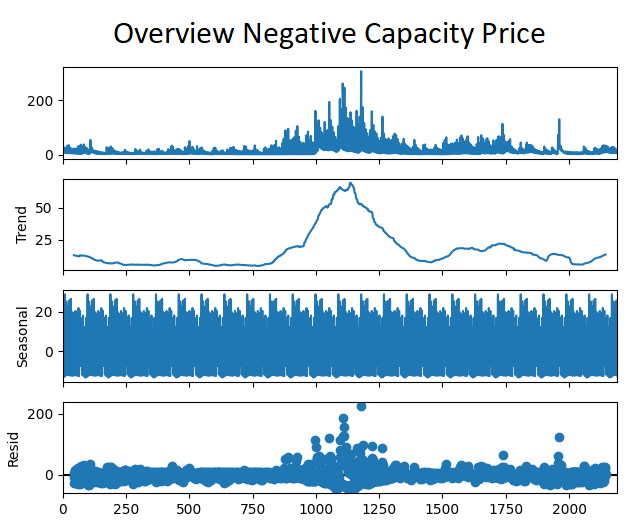
\includegraphics[width=0.7\linewidth]{pictures/capacityData_overview.png}
	\caption{Total Average Negative Capacity Price}
	\label{fig:Overview Average Negativ Capacity Price}
\end{figure}

A more detailed examination of the seasonality reveals both a daily
and a slight weekly rhythm in the data. Since the dataset refers to 4-hour blocks, every six time lags
correspond to a full day. Figure~\ref{fig:Autocorrelation Negative Capacity Price - 5 Days}
clearly illustrates the presence of a daily pattern in the autocorrelation of the data.

\begin{figure}[!h]
	\centering
	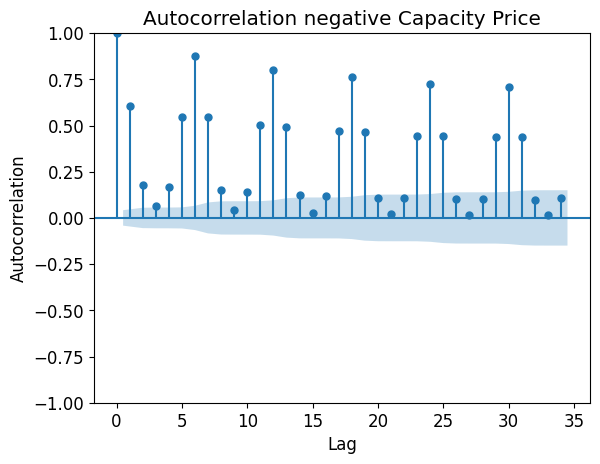
\includegraphics[width=0.7\linewidth]{pictures/Autocorrelation negative Capacity Price.png}
	\caption{Autocorrelation Negative Capacity Price – 5 Days}
	\label{fig:Autocorrelation Negative Capacity Price - 5 Days}
\end{figure}

Moreover, Figure \ref{fig:AutocorrNegCap4Weeks} indicates a moderate weekly cycle.

\begin{figure}[!h]
	\centering
	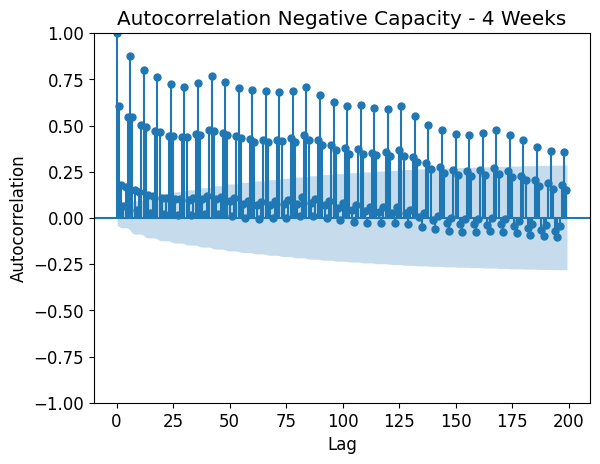
\includegraphics[width=0.7\linewidth]{pictures/Autocorrelation Negative Capacity - 4 Weeks.png}
	\caption{Autocorrelation Negative Capacity Price – 4 Weeks}
	\label{fig:AutocorrNegCap4Weeks}
\end{figure}

The price development for positive capacity shows a similar behavior
to that of the negative capacity prices.

Given the strong autocorrelation in the data, several statistical methods are well-suited
for time series analysis and forecasting. In particular, the ARIMA method,
which is based on autoregression, proves to be effective for time series
with strong autocorrelation. To better account for seasonal effects,
a seasonal variant of the ARIMA method SARIMA can be applied.
But SARIMA struggles with complexity in long time series:
computation times increased exponentially, and long-term forecasts tended to be biased
towards the most recent trend.
Since we expect similar annual patterns in the short term, this bias toward the latest trend
is considered unrealistic and undesirable.
Moreover, SARIMA is inherently limited to modeling a single seasonal component.
To account for multiple seasonalities, extensive manual adjustments would be necessary.

A more flexible alternative is the TBATS algorithm, which builds upon similar principles
while overcoming these limitations. TBATS stands for Trigonometric seasonality,
Box-Cox transformation, ARMA errors, Trend, and Seasonal components.
It is implemented in the SKTIME framework and enables efficient forecasting
of time series with multiple seasonal patterns~\cite{.05.04.2025}.

The resulting forecasted time series closely resembles the actual historical time series
(Figure~\ref{fig:Negative Capacity Price Prediction - 2023}).
Note that the time series shown here corresponds to the most probable scenario—
meaning that 50\% of all possible forecast values lie above, and 50\% lie below the prediction.

When generating longterm forecast scenarios using the trained predictor,
the inherent uncertainty increases with forecasting horizon,
resulting in a wider prediction interval
(Figure~\ref{fig:Negative Capacity Price Prediction Interval - 2023}).
While this is methodologically sound and suitable for many use cases,
we assume that the mean forecast does not lose accuracy over time
and use it as the basis for scenario generation.

\begin{figure}[!h]
	\centering
	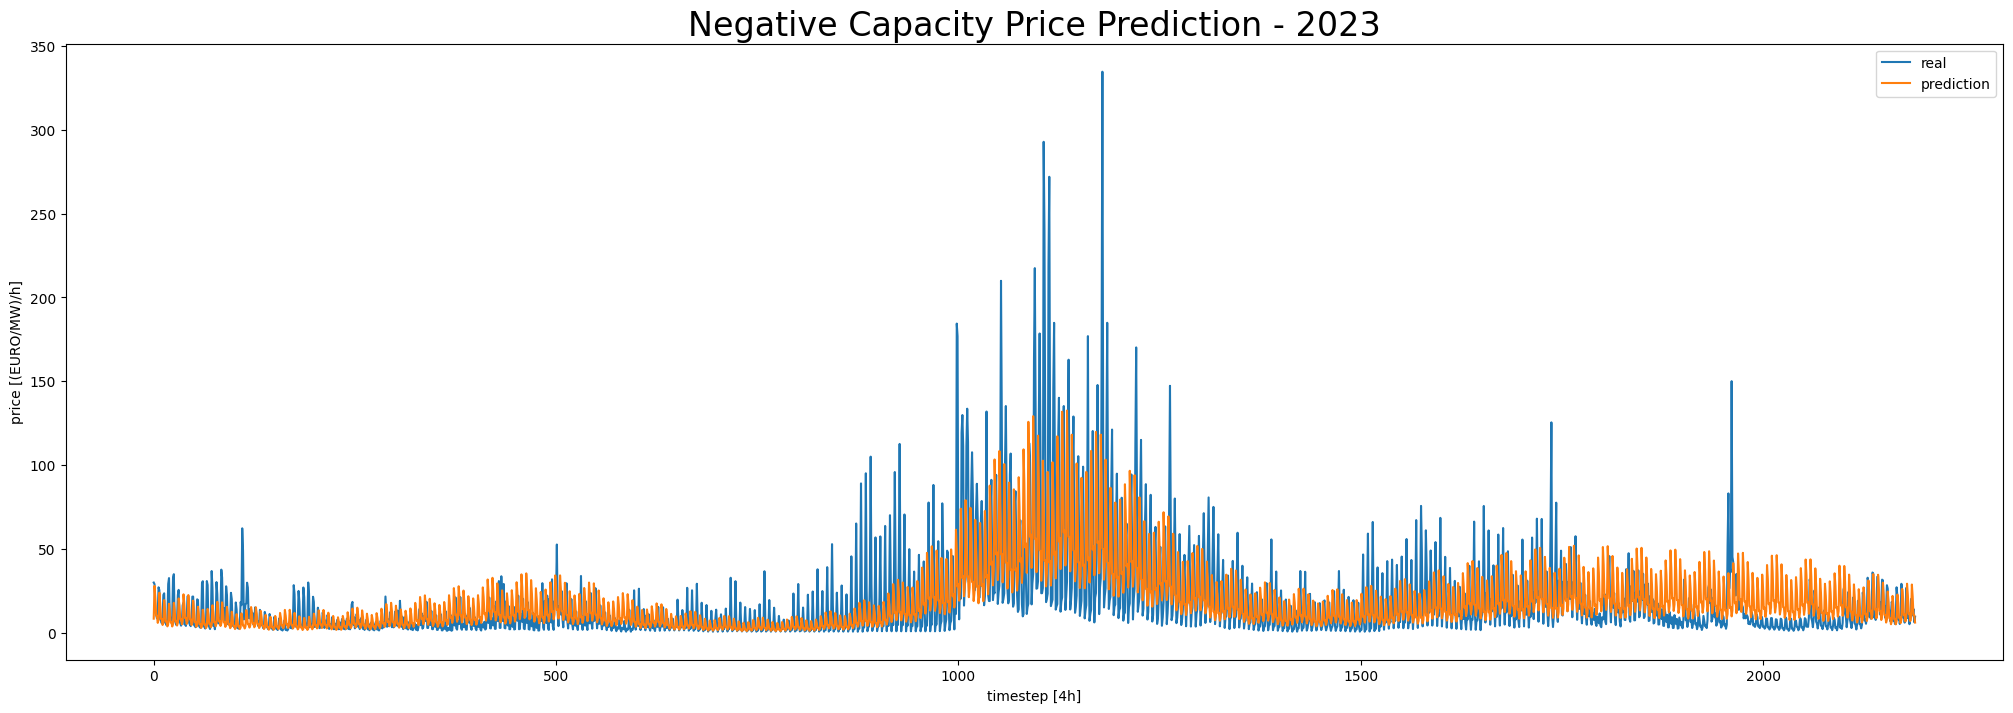
\includegraphics[width=1\linewidth]{pictures/RL/Negative Capacity Price Prediction - 2023.png}
	\caption{Negative Capacity Price Prediction – 2023}
	\label{fig:Negative Capacity Price Prediction - 2023}
\end{figure}

\begin{figure}[H]
	\centering
	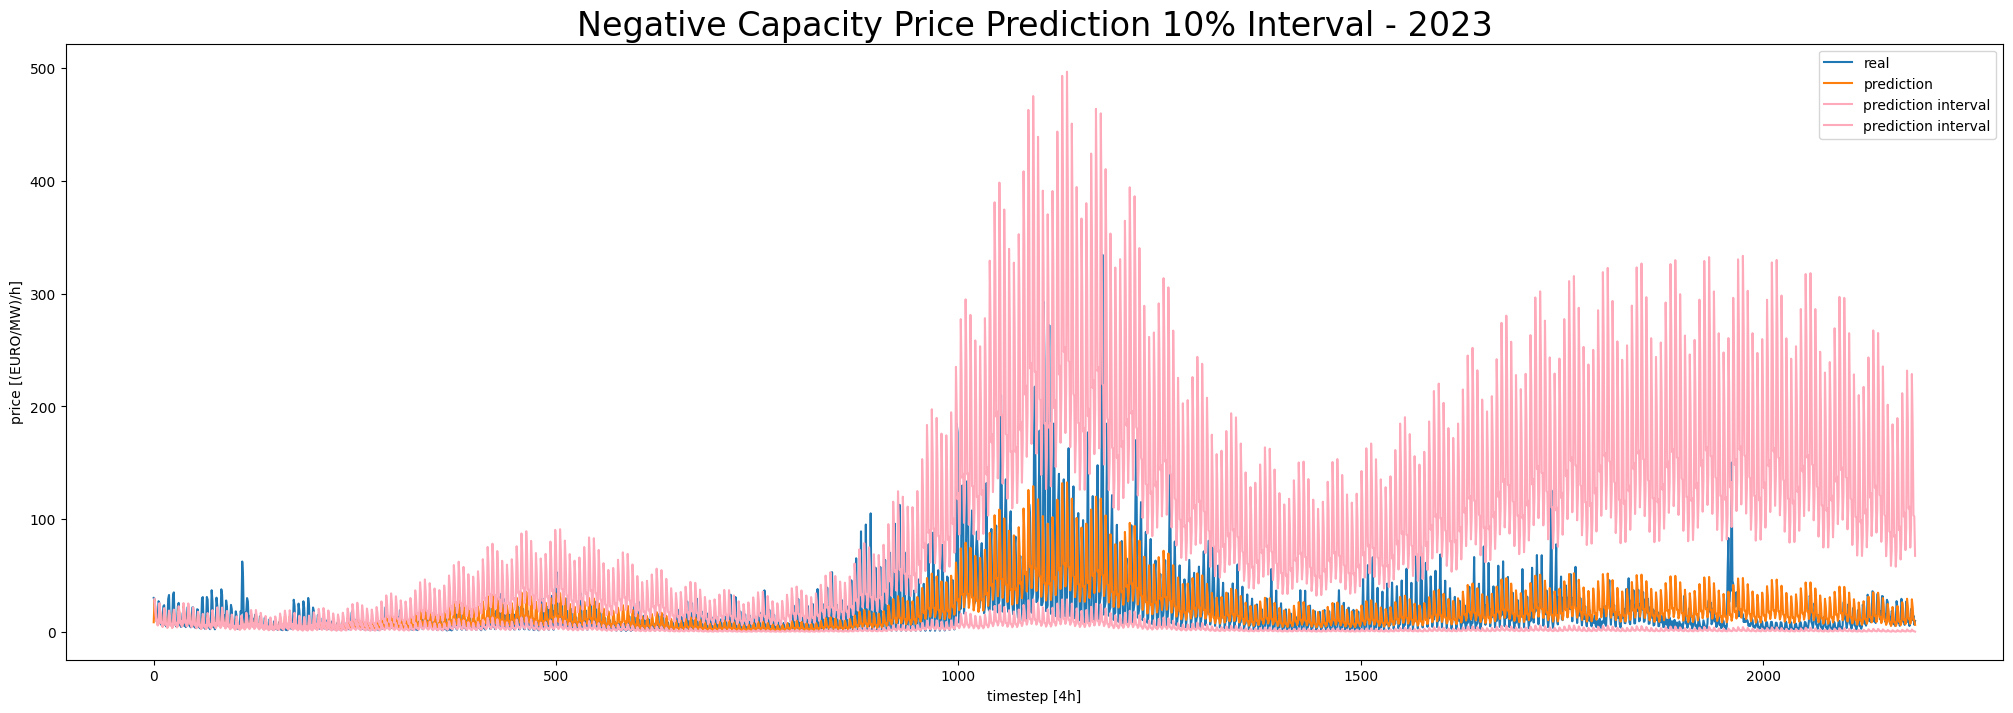
\includegraphics[width=1\linewidth]{pictures/RL/Negative Capacity Price Prediction Interval - 2023.png}
	\caption{Negative Capacity Price Prediction 10\%-Interval – 2023}
	\label{fig:Negative Capacity Price Prediction Interval - 2023}
\end{figure}

For scenario generation, the median forecast is used and manually scaled upward and downward (e.g., by ±10\%).
These scaled series are then evaluated to determine in how many cases a bidding success would have occurred.


\subsection{Day Ahead Market}

Although the Day-Ahead market prices are variable, they exhibit a daily and weekly rhythm.
Over the course of the year, only general trends are observable, as shown in Figure~\ref{fig:overviewDAprices}.

\begin{figure}[!h]
	\centering
	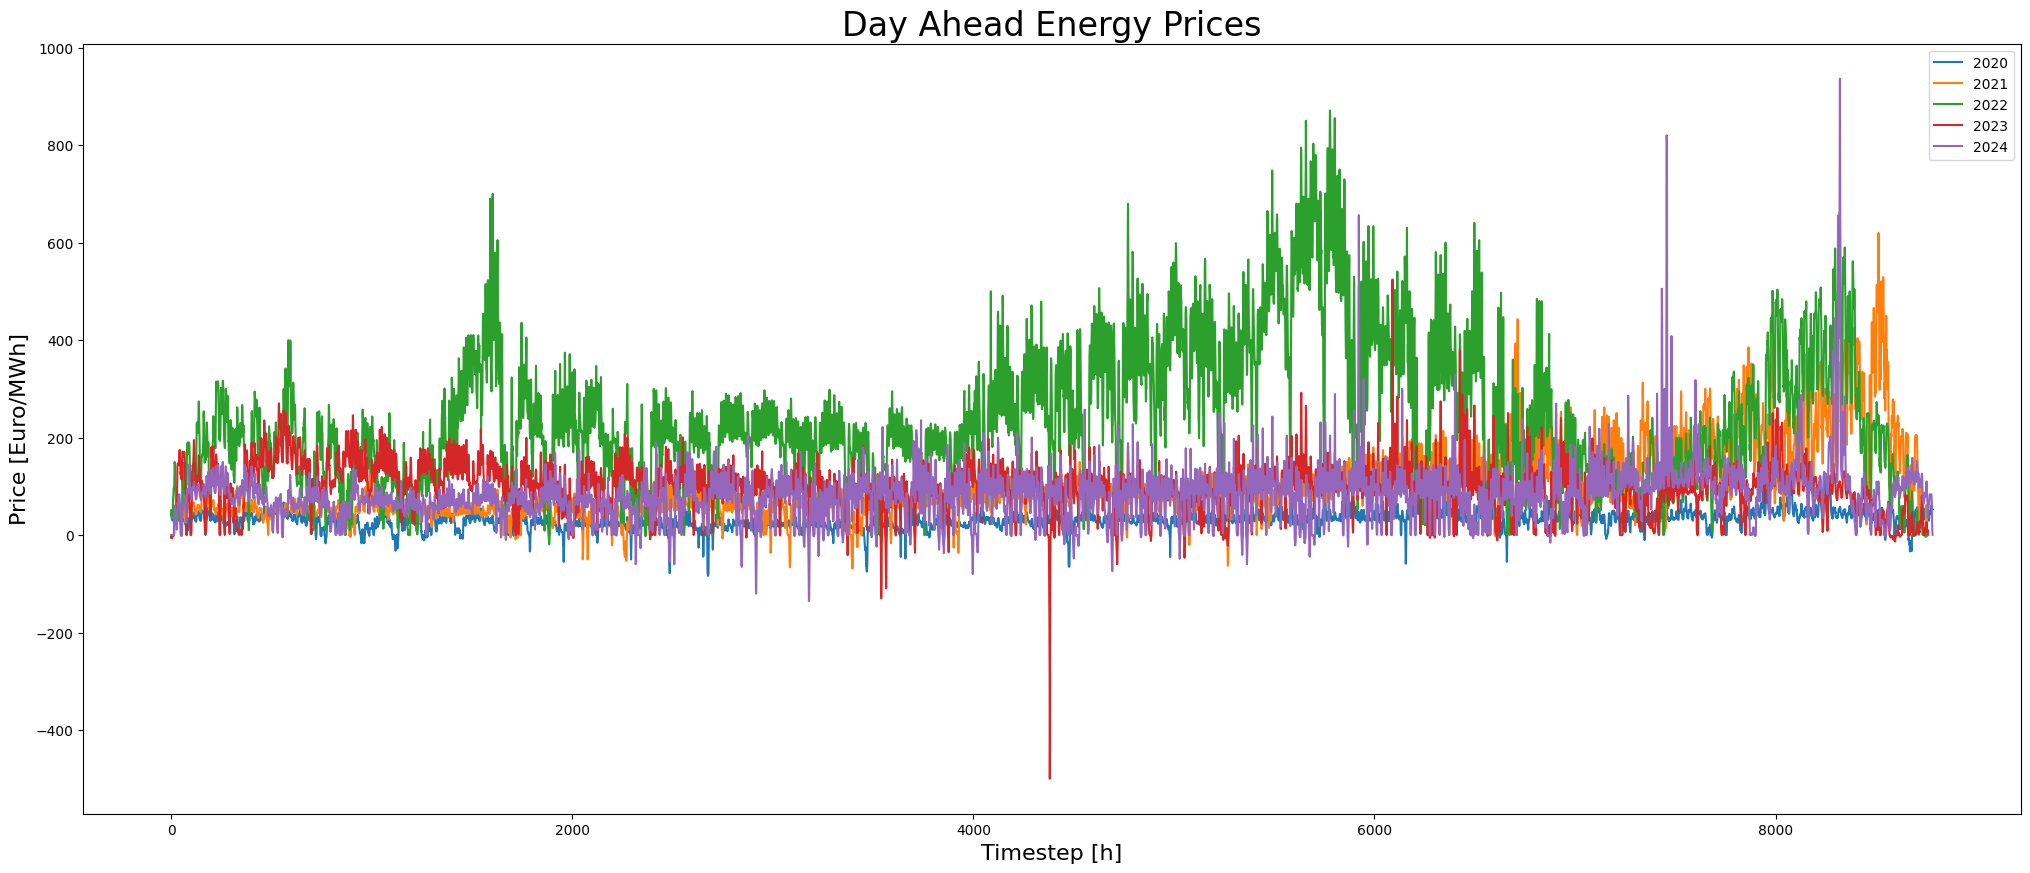
\includegraphics[width=1\linewidth]{pictures/overviewDAprices_year.png}
	\caption{Overview DA prices}
	\label{fig:overviewDAprices}
\end{figure}
\todo{redo figure with bigger legend}

The extraordinary curve movement observed in 2022 (green curve) can be attributed to
Russia's war of aggression against Ukraine and the resulting turmoil
in the gas market.

Since the Day-Ahead (DA) market operates on a pay-as-cleared mechanism
(i.e., all participants receive the price of the highest accepted bid),
and we act as a producer of renewable energy with very low operational costs,
the model only needs to consider whether we participate in the market
and what the expected clearing price is.

As illustrated in Figures \ref{fig:meanDA2020} to \ref{fig:stdDA2024},
the clearing price exhibits both daily and weekly periodicities.
While the overall level of prices may vary, the pattern remains predictable.
Due to the market design, it is sufficient for our model to rely
on an expected clearing price, as we can realistically submit
a zero-price bid and are therefore almost guaranteed to be dispatched.

The expected price used in our model is calculated as the average
of the years 2020 through 2024, excluding 2022. This approach
preserves the seasonal structure of the data while smoothing out
extreme outliers in both directions. Consequently, a reliably
expected clearing price can be determined based on time of day,
day of the week, and time of year.

Furthermore, the price level can be adjusted afterward using
a simple scaling factor without compromising the inherent
structure of the data.


\begin{figure}[H]
	\centering
	\begin{minipage}{0.49\textwidth}
		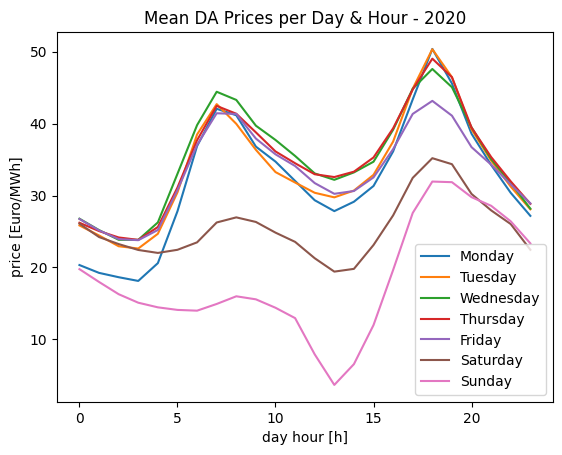
\includegraphics[width=1\linewidth]{pictures/DA/Mean DA Prices per Day and Hour - 2020.png}
		\subcaption{Mean DA-Price}
		\label{fig:meanDA2020}
	\end{minipage} \hfill
	\begin{minipage}{0.49\textwidth}
		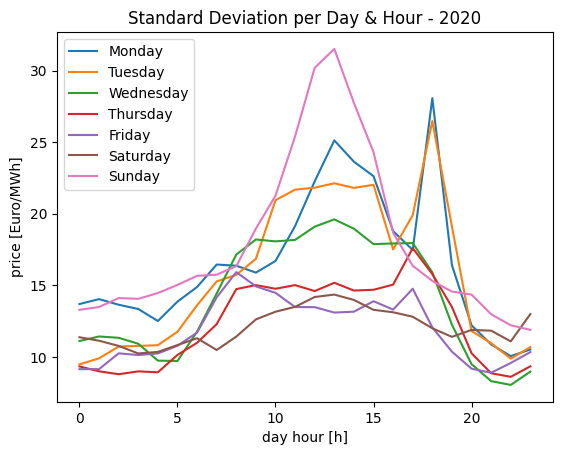
\includegraphics[width=1\linewidth]{pictures/DA/Standard Deviation per Day and Hour - 2020.png}
		\subcaption{Standard Deviation DA-Price}
		\label{fig:stdDA2020}
	\end{minipage}
	\caption{Daily and hourly DA-Data - 2020 }
\end{figure}

\begin{figure}[H]
	\centering
	\begin{minipage}{0.49\textwidth}
		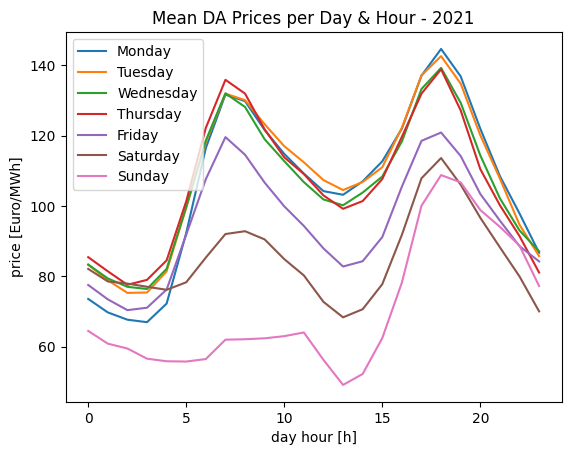
\includegraphics[width=1\linewidth]{pictures/DA/Mean DA Prices per Day and Hour - 2021.png}
		\subcaption{Mean DA-Price }
		\label{fig:meanDA2021}
	\end{minipage} \hfill
	\begin{minipage}{0.49\textwidth}
		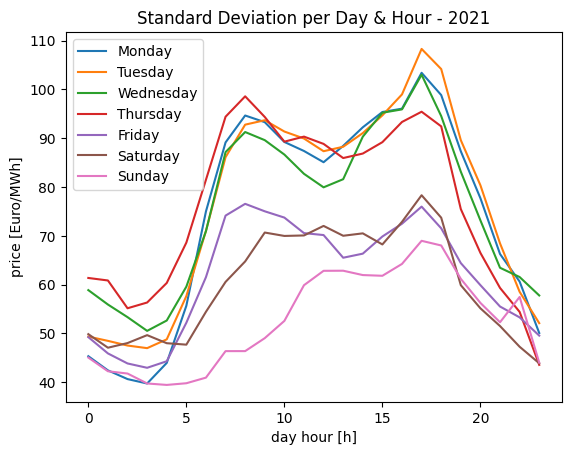
\includegraphics[width=1\linewidth]{pictures/DA/Standard Deviation per Day and Hour - 2021.png}
		\subcaption{Standard Deviation DA-Price}
		\label{fig:stdDA2021}
	\end{minipage}
	\caption{Daily and hourly DA-Data - 2021 }
\end{figure}

\begin{figure}[H]
	\centering
	\begin{minipage}{0.49\textwidth}
		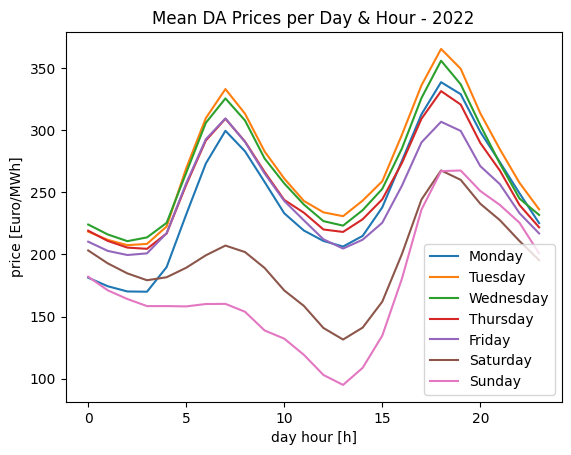
\includegraphics[width=1\linewidth]{pictures/DA/Mean DA Prices per Day and Hour - 2022.png}
		\subcaption{Mean DA-Price }
		\label{fig:meanDA2022}
	\end{minipage} \hfill
	\begin{minipage}{0.49\textwidth}
		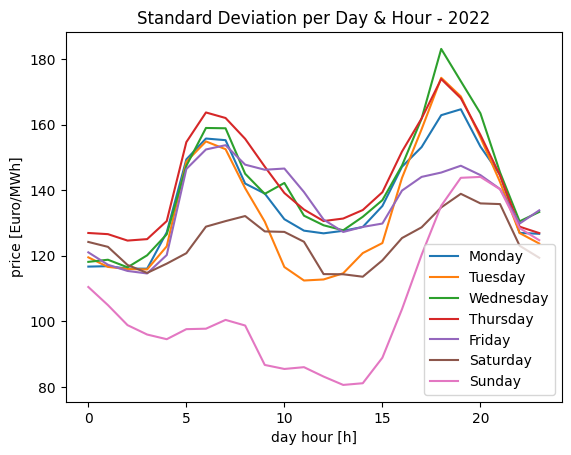
\includegraphics[width=1\linewidth]{pictures/DA/Standard Deviation per Day and Hour - 2022.png}
		\subcaption{Standard Deviation DA-Price}
		\label{fig:stdDA2022}
	\end{minipage}
	\caption{Daily and hourly DA-Data - 2022 }
\end{figure}

\begin{figure}[H]
	\centering
	\begin{minipage}{0.49\textwidth}
		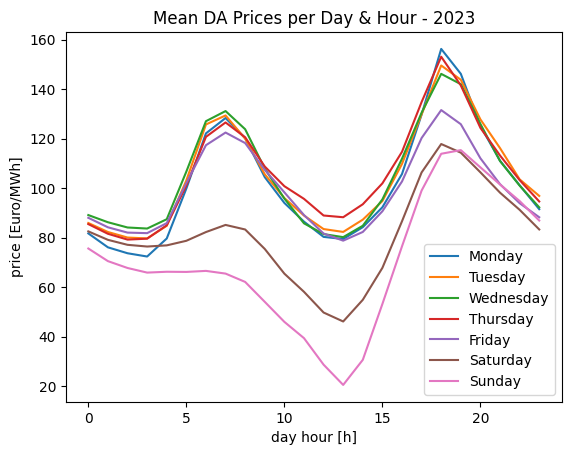
\includegraphics[width=1\linewidth]{pictures/DA/Mean DA Prices per Day and Hour - 2023.png}
		\subcaption{Mean DA-Price }
		\label{fig:meanDA2023}
	\end{minipage} \hfill
	\begin{minipage}{0.49\textwidth}
		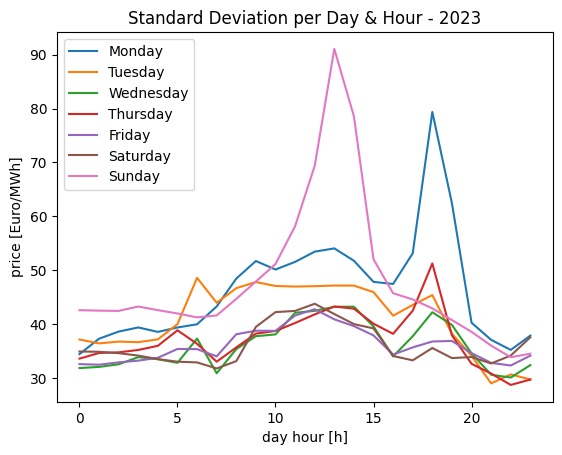
\includegraphics[width=1\linewidth]{pictures/DA/Standard Deviation per Day and Hour - 2023.png}
		\subcaption{Standard Deviation DA-Price}
		\label{fig:stdDA2023}
	\end{minipage}
	\caption{Daily and hourly DA-Data - 2023 }
\end{figure}

\begin{figure}[H]
	\centering
	\begin{minipage}{0.49\textwidth}
		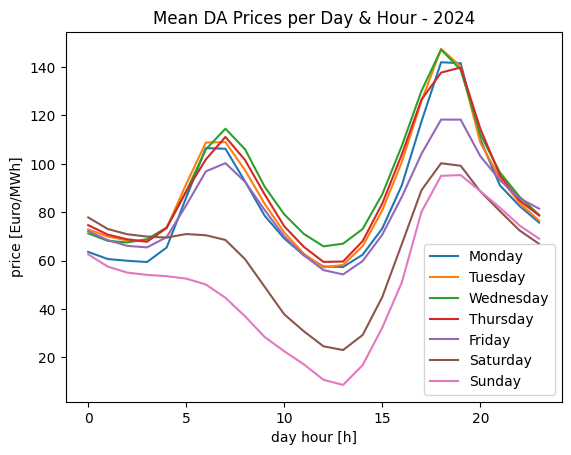
\includegraphics[width=1\linewidth]{pictures/DA/Mean DA Prices per Day and Hour - 2024.png}
		\subcaption{Mean DA-Price }
		\label{fig:meanDA2024}
	\end{minipage} \hfill
	\begin{minipage}{0.49\textwidth}
		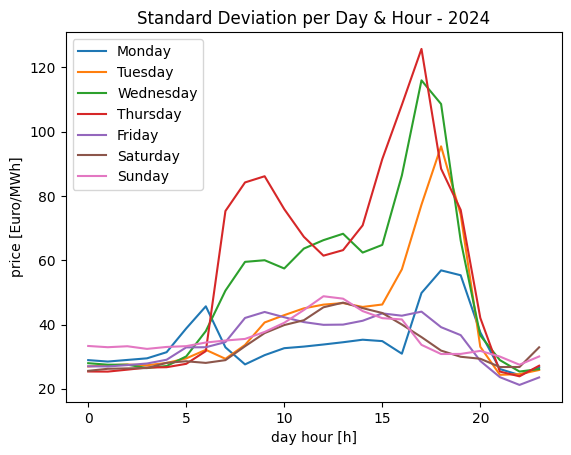
\includegraphics[width=1\linewidth]{pictures/DA/Standard Deviation per Day and Hour - 2024.png}
		\subcaption{Standard Deviation DA-Price}
		\label{fig:stdDA2024}
	\end{minipage}
	\caption{Daily and hourly DA-Data - 2024 }
\end{figure}

Additionally, for the purpose of our simulation, we assume that the
simulated renewable energy system represents an onshore wind farm
located in Germany. To obtain a wind profile, we divide the total
onshore wind power generation by the total installed capacity
of these systems \cite{.08.04.2025}.

The resulting profile reflects the mean relative wind power output over the entire
country. Because wind turbines across Germany are rarely
operating simultaneously at zero or full capacity, there are no peaks in this view.
In contrast, for an individual wind park, full or zero output can indeed occur. Therefore, in order to give
the constraint on maximum grid connection capacity a meaningful interpretation,
this average profile needs to be rescaled.

To this end, we treat the national wind production as a proxy for
the wind conditions at our specific location. We then apply a scaling
transformation that compresses the lower values and expands the higher ones.
An additional requirement of the transformation is that the maximum values
should be normalized to 1, which corresponds to our wind park operating
at full capacity.

This is achieved by first subtracting the mean of the national wind
profile, resulting in a series of positive and negative deviations.
We then apply a scaling factor to amplify these deviations both
upward and downward. Afterward, we add back the original mean to preserve
the average and total energy content of the original profile.
This transformation yields a new time series whose average matches
the original, but whose minimum is 0 and maximum value reaches 1 [\ref{eq:windProfil_our}].


\begin{flalign}
	wp_{our} = ((wp_{ger} - \bar{wp_{ger}}) * wsf) + \bar{wp_{ger}} \label{eq:windProfil_our}
\end{flalign}

The scaling factor is calculated as follows:

\begin{flalign}
	wsf = \frac{1-\bar{wp_{ger}}}{\max(wp_{ger}) - \bar{wp_{ger}}} \label{eq:windProfil_wsf}
\end{flalign}


\subsection{aFFR - Energy}
\label{chap:affR_energy}

The aFFR energy market exhibit a high degree of variability and are extremely difficult to predict statistically.
As such, they exhibit only a very weak autocorrelation, with only a slight daily rhythm, as shown in Figure
\ref{fig:Autocorrelation Positive Energy Price} (1 lag = 15 min).

\begin{figure}[!h]
	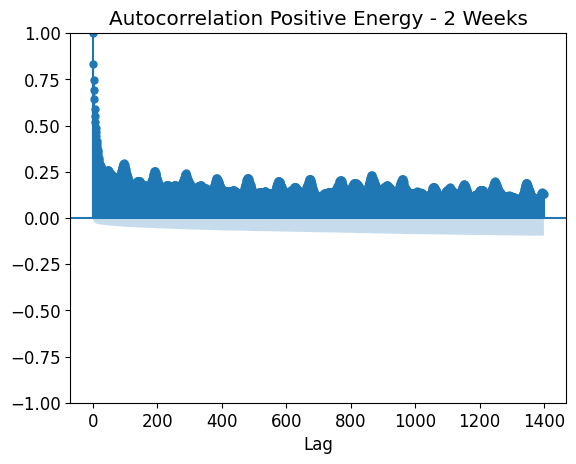
\includegraphics[width=1\linewidth]{pictures/Autocorrelation Positive Energy - 2 Weeks.png}
	\caption{Total Average Positive Energy Price}
	\label{fig:Autocorrelation Positive Energy Price}
\end{figure}

No trends are present in the data either.
As shown in Figure \ref{fig:posEngOverview}, we present 30-day samples from the early, middle, and late parts of the year.
In these periods, neither trends nor seasonal developments are observable.

\begin{figure}[!h]
	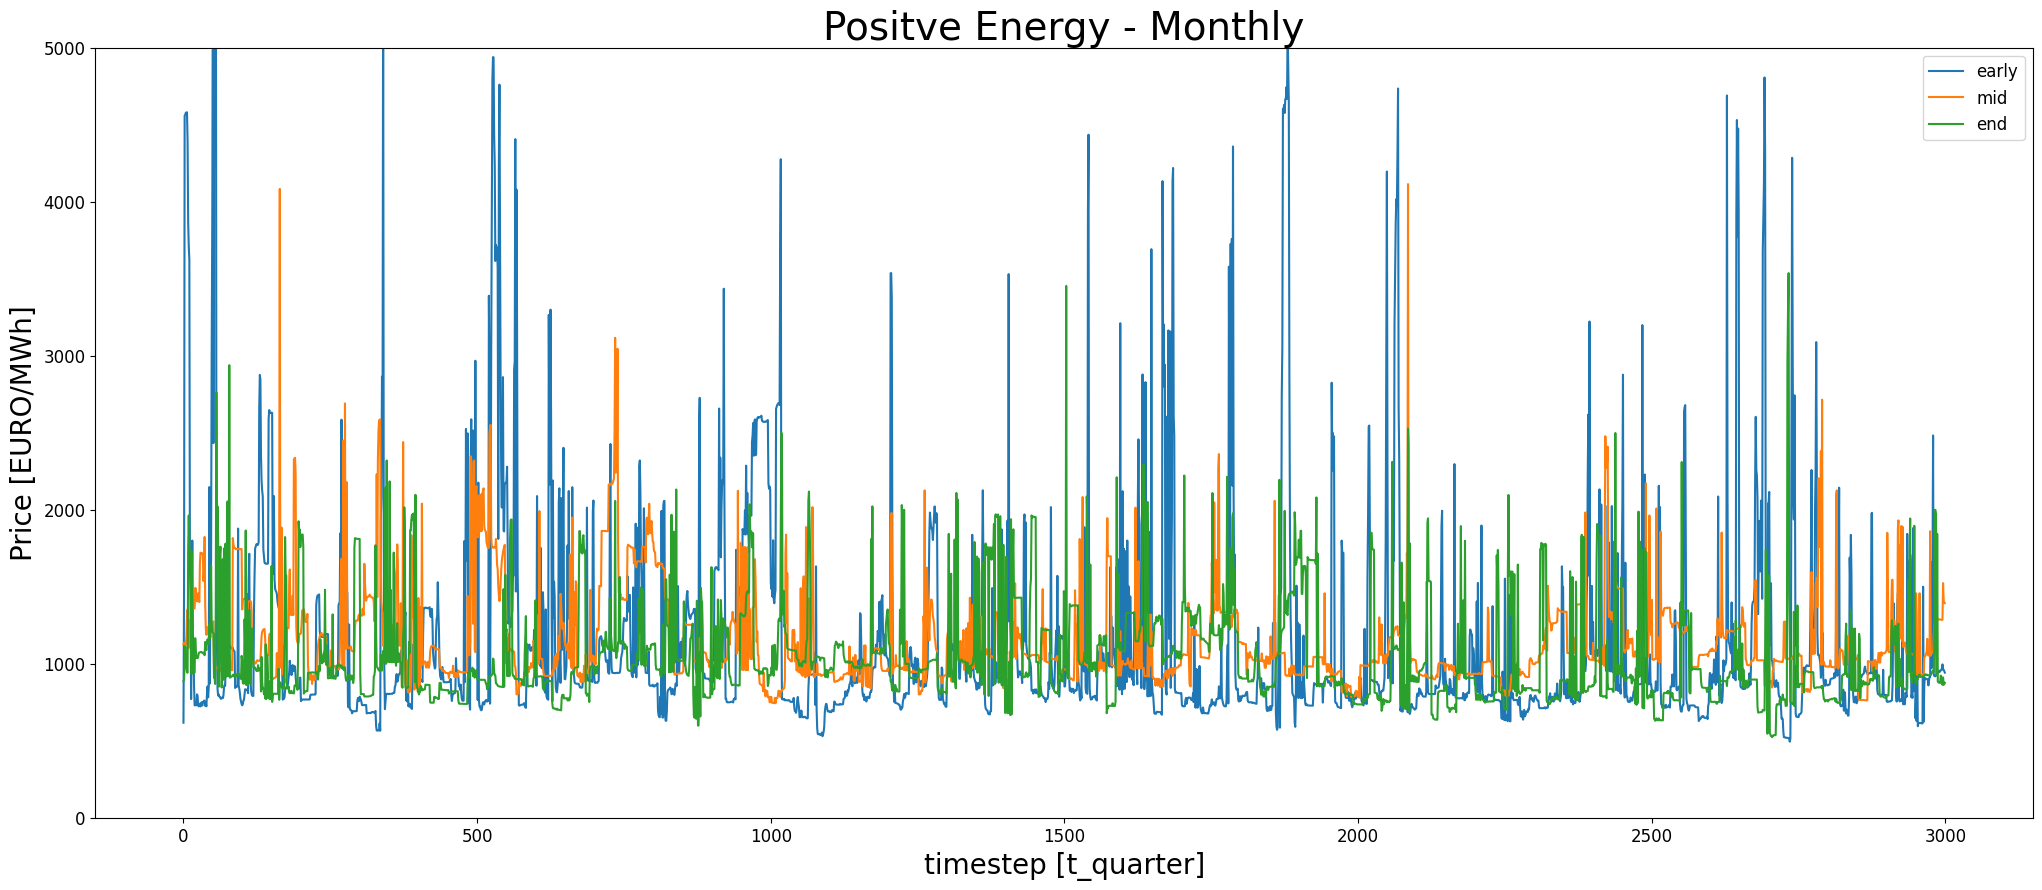
\includegraphics[width=1\linewidth]{pictures/posEngOverview.png}
	\caption{Overview Positive Energy Price}
	\label{fig:posEngOverview}
\end{figure}
\todo{das ist eine grafik mit den alten average preise, mache eine graifk mit den richtigen grenzpreisen}
\todo{grafiken verschiedene Preisszenarien}
\todo{appendix verweis zu python code}

Since no reliable forecasts can be made, real-world data is used for scenario generation.
For this purpose, data from the year 2023 was employed [see Table \ref{tab:energy_sources_std}].
It is observed that solar and onshore wind power plants are particularly subject to volatile production patterns.

\begin{table}[ht]
	\centering
	\begin{tabular}{|l|r|}
		\hline
		\textbf{Source}                 & \textbf{Standard Deviation} \\
		\hline
		Geothermal                      & 5.956190                    \\
		Fossil Oil                      & 85.360298                   \\
		Waste                           & 133.320136                  \\
		Hydro Water Reservoir           & 167.126363                  \\
		Hydro Run-of-river and poundage & 310.405850                  \\
		Biomass                         & 429.594441                  \\
		Nuclear                         & 1223.169733                 \\
		Hydro Pumped Storage            & 1543.402759                 \\
		Wind Offshore                   & 1833.588012                 \\
		Fossil Gas                      & 2916.794393                 \\
		Fossil Hard coal                & 3364.505964                 \\
		Fossil Brown coal/Lignite       & 3799.694920                 \\
		\textbf{Solar}                  & \textbf{9879.907341}        \\
		\textbf{Wind Onshore}           & \textbf{10506.831136}       \\
		\hline
	\end{tabular}
	\caption{Standard deviation per energy generator type}
	\label{tab:energy_sources_std}
\end{table}

Subsequently, the total production from solar and onshore wind is calculated for each time point,
and divided by the total production of all power plants at the same time.
This provides the relative share of these particularly volatile power plants in the overall production.
The relative hourly production is then used to determine daily average values.

The hypothesis is that if a prediction error occurs, it has a particularly strong impact when it occurs on days
with a high share of volatile production in the overall output.

These relative production data of volatile power plants are then divided into 36 quantiles.
The first, median, and last quantiles are used for scenario generation.

For this, the time points of the quantiles, now based on daily data, are extrapolated to a quarter-hourly rhythm,
and the corresponding market data from the other markets for the respective time periods are exported.
Simultaneously, the matching time periods from the DA and aFFR time series are also exported.

This results in 10 possible scenarios for days with high, medium, and low shares of volatile production.
The probabilities are assumed to be evenly distributed, thus each scenario-day has a probability of 10\%.


The entire python code and origin data used can be found in Appendix~\ref{app:python}


\section{Simplifications}
\label{chap:Simplifications}
In this study, we assume the role of a participant within a bidding consortium.
As such, minimum bid requirements can be disregarded,
as we assume our consortium partners to be sufficiently large to always meet these minimum thresholds.

To manage the computational effort and reduce the model's complexity, several simplifications have been implemented.
These simplifications do not substantially compromise the realism of the model.
The following is a structured list of the simplifications employed.

\subsubsection{aFFR Capacity/DA Quantile Data}
For the time series analyzed, it is important to note that the values are determined based on the preceding day.
As a result, the prediction error for the following day has not yet materialized.
Consequently, the quantile data for the day ahead aFFR capacity can be averaged over the 10 scenarios days.
This approach minimizes unnecessary complexity and allows for more general,
strategic conclusions to be drawn regarding bidding behavior in the aFFR capacity/DA market,
in relation to potential high, medium, and low prediction errors.

\subsubsection{Day Ahead Market}
Since the Day-Ahead market operates under a pay-as-cleared structure, our bid influences only the acceptance or rejection of our offer,
with no impact on the price paid for the electricity.
Given our assumption that we operate a wind farm, we consider operational costs to be negligible, and thus, assume them to be zero.
As Day-Ahead prices are non-negative, we can effectively choose whether to submit a bid at a price that will almost certainly be accepted.
This results in a simplified optimization for the DA market, represented by $Profit_{Da} = Q_{DA} * p^{exp}_{DA}$.
We further assume our specific renewable production forecast as perfect.

\subsubsection{aFFR Energy Market}
As the aFFR Energy Market market also follows a pay-as-cleared principle, our bid influences only whether we are called upon to deliver, with no impact on the price paid for the electricity.
Assuming the role of a battery storage operator with near-zero operational costs, these are considered negligible.
Thus, we can submit a bid below the expected RA market price to ensure that our offer is likely to be called.
The reverse is also true.

When an aFFR capacity bid is accepted, we are obligated to submit a corresponding aFFR energy bid.
This creates a constraint that limits the minimum bid quantity in the aFFR energy market based on the accepted aFFR capacity bid quantity.
However, integrating the introduced case would lead to an increase in computational complexity due to the need for extra variables and additional
dimensions. In practice, this regulatory constraint can be bypassed by setting a sufficiently high working price, ensuring that our bid is not called upon.
Therefore, this constraint was not explicitly incorporated into the model.
But, we incorporated a constraint that links the minimum and maximum $BatStat$ to the accepted aFFR energy bids.
This ensures that, at all times during the relevant aFFR block, sufficient storage capacity is available to fulfill any potential requests.
This approach avoids the computationally intensive direct linkage between the aFFR capacity and aFFR energy markets while still
accurately reflecting the underlying mechanisms.

\subsubsection{Battery Storage Status}



The battery storage status is recalculated at 15-minute intervals.
The battery status from the previous time window is updated by adding all inflows and subtracting all outflows.
Given the uncertainty of these inflows and outflows, multiple possible battery states would arise at the end of each calculation window, based on the possible preceding states.
Since we calculate the battery status over 96 consecutive time periods, the computational complexity would increase exponentially due to the number of possible outcomes over these 96 periods.
Even with only two considered scenario outputs, this results in
\[
	2^{96} = 79228162514264337593543950336
\]
possible battery storage states at the end of the day.
Considering that planning always takes place for the following day,
one would need to account for
\[
	2^{182} = 6.13 \times 10^{54}
\]
possible battery storage states before achieving planning certainty again.
Since a full enumeration of all possible future system states quickly becomes computationally infeasible,
it is necessary to either assume perfect foresight and calculate a single, most probable trajectory
for the battery storage system, or to approximate certain processes along the time series.
Therefore, we approximate the battery storage calculation by determining an expected battery status at time $t_quarter$ and using this expected value for subsequent calculations.
Inflows and outflows are weighted by their respective probabilities, allowing for an approximation of the correct battery status over the entire period.

This method inherently flattens the battery loading status curve, depending on the assumed probability distributions.
For example in reality, consecutive 10\% fluctuations may occur, leading to a more pronounced shift in the battery status than the model predicts.
To ensure that the storage capacity meets the required levels, the actual capacity have to be recalculated by considering unweighted quantity bids and determining the maximum fluctuation.
This value corresponds to the actual required storage capacity.
As the storage/bid ratio increases, the impact of this adjustment becomes negligible, as the likelihood of consecutive unlikely events diminishes over time.


\include{chapters/model_eng.tex}
\chapter{Results}

\todo{beachten das das die durchschnittlichen q's über alle möglichen szenarion innerhalb des erwarteten quantils sind}
To properly contextualize the results, we begin by briefly presenting the initial data.

\todo{neue DA markt linie}

The relative production quantiles, which were used to segment the other time series, are illustrated as follows:

\begin{figure}[!h]
	\centering
	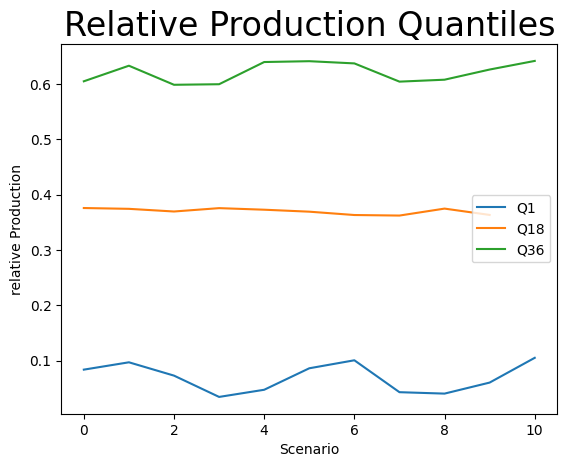
\includegraphics[width=0.7\linewidth]{pictures/results/relativeProduktionQuantils.png}
	\caption{Relative Production Quantiles}
	\label{fig:Relative Production Quantiles}
\end{figure}

Based on these, the resulting time series for activated balancing energy and their corresponding prices are shown below:
The corresponding data for the aFFR market is presented in the Appendix~\ref{chap:app_QaFFRmarketData}
The data indicate that, with increasing market penetration of volatile energy sources, the volume of activated negative balancing energy increases,
whereas the demand for positive balancing energy tends to decrease.
A similar pattern emerges in the marginal prices for activated balancing energy.
While the prices for negative balancing energy rise with a higher share of volatile producers,
the prices for positive balancing energy decline.
Notably, there are significant outliers in the time series of marginal prices for positive balancing energy,
especially in scenarios with medium and low market penetration of volatile producers.

The median \todo{perhaps add a clarification in the data section as to why medians are used here} balancing capacity prices peak for
both negative and positive in the medium volatility scenario.
In the first quantile's data, the prices for negative capacity are comparable to those in the 36th quantile.
For positive balancing energy, however, the 36th quantile diverges significantly from the 1st quantile,
especially during the later hours of the day.

Based on these time series, the model produced the following results:

The bidding strategy for capacity market prices consistently remains just below the expected marginal price across all scenarios.
\todo{insert graphic here ... !! rather important !!}

It can be observed that the provision of negative balancing energy occurs earlier in the low and medium scenarios
when both balancing power bids are accepted [Figure \ref{fig:Negative Balance Energy - Q1}, \ref{fig:Negative Balance Energy - Q18}].
This temporal shift is not observed in scenarios with high volatility energy production penetration [Figure \ref{fig:Negative Balance Energy - Q36}].

While the bidding quantities for positive balancing energy remain largely consistent across low and medium volatility scenarios,
regardless of capacity market acceptance, more pronounced differences appear under high-volatility conditions.
In these scenarios, earlier energy provision also results from tighter restrictions due to capacity market results.

To aid in interpretation, we define the following restriction categories:
\begin{enumerate}
	\item Restricted: B $\rightarrow$ RL accepted for both input and output (blue)
	\item Restricted: O $\rightarrow$ RL accepted for output, declined for input (orange)
	\item Restricted: I $\rightarrow$ RL accepted for input, declined for output (green)
	\item Restricted: N $\rightarrow$ RL declined for both input and output (red)
\end{enumerate}

The results indicate a relatively consistent bidding behavior in the capacity market across all scenarios.

\begin{figure}[!h]
	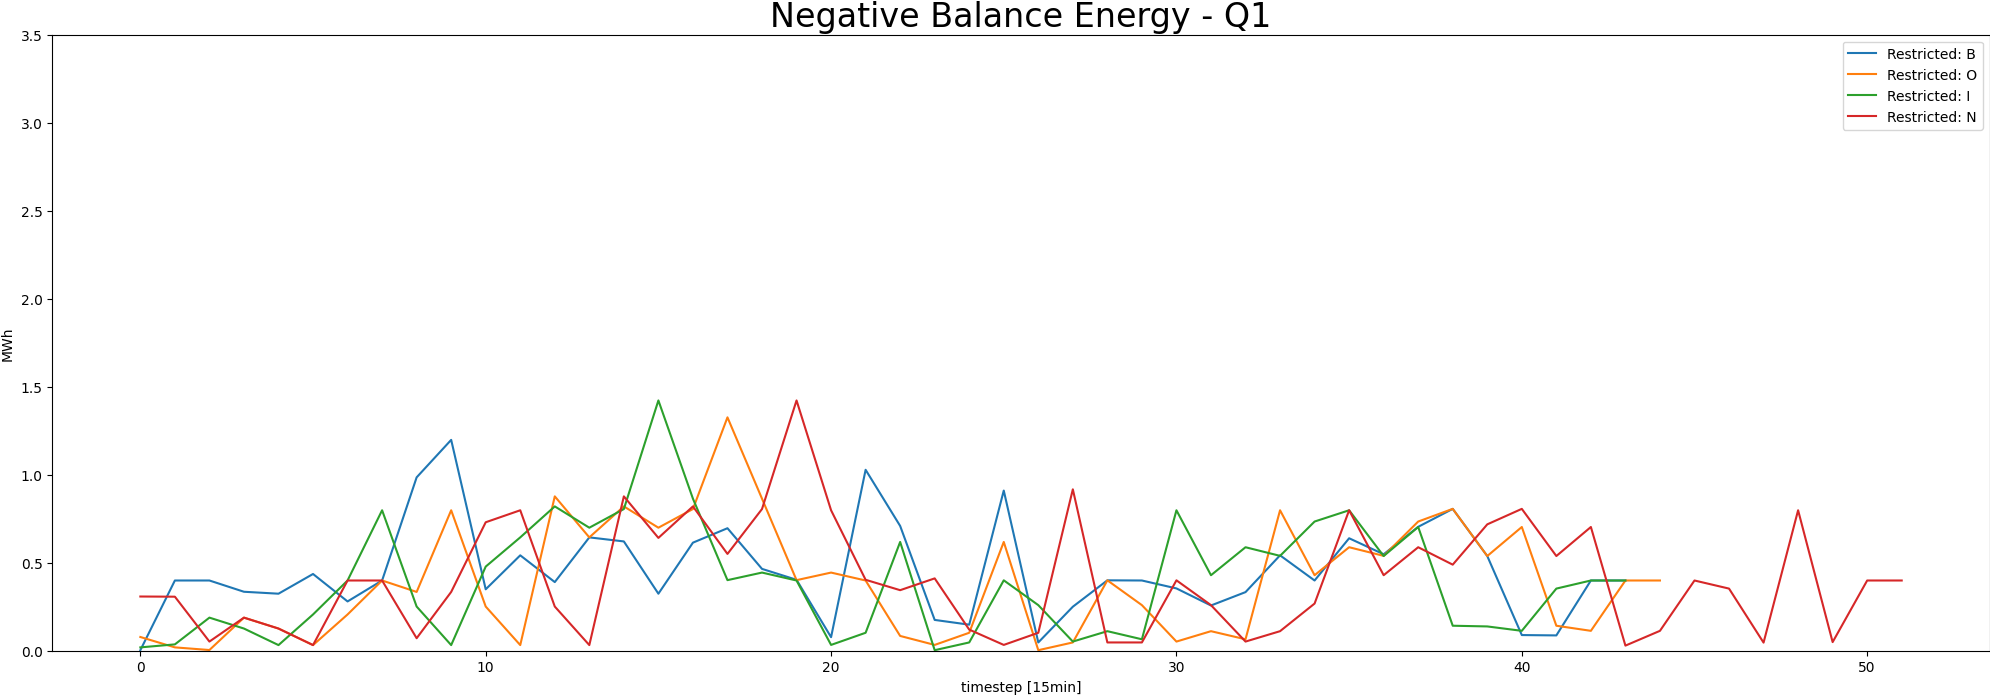
\includegraphics[width=1\linewidth]{pictures/results/Negative Balance Energy - Q1.png}
	\caption{Negative Balance Energy - Q1}
	\label{fig:Negative Balance Energy - Q1}
\end{figure}

\begin{figure}[!h]
	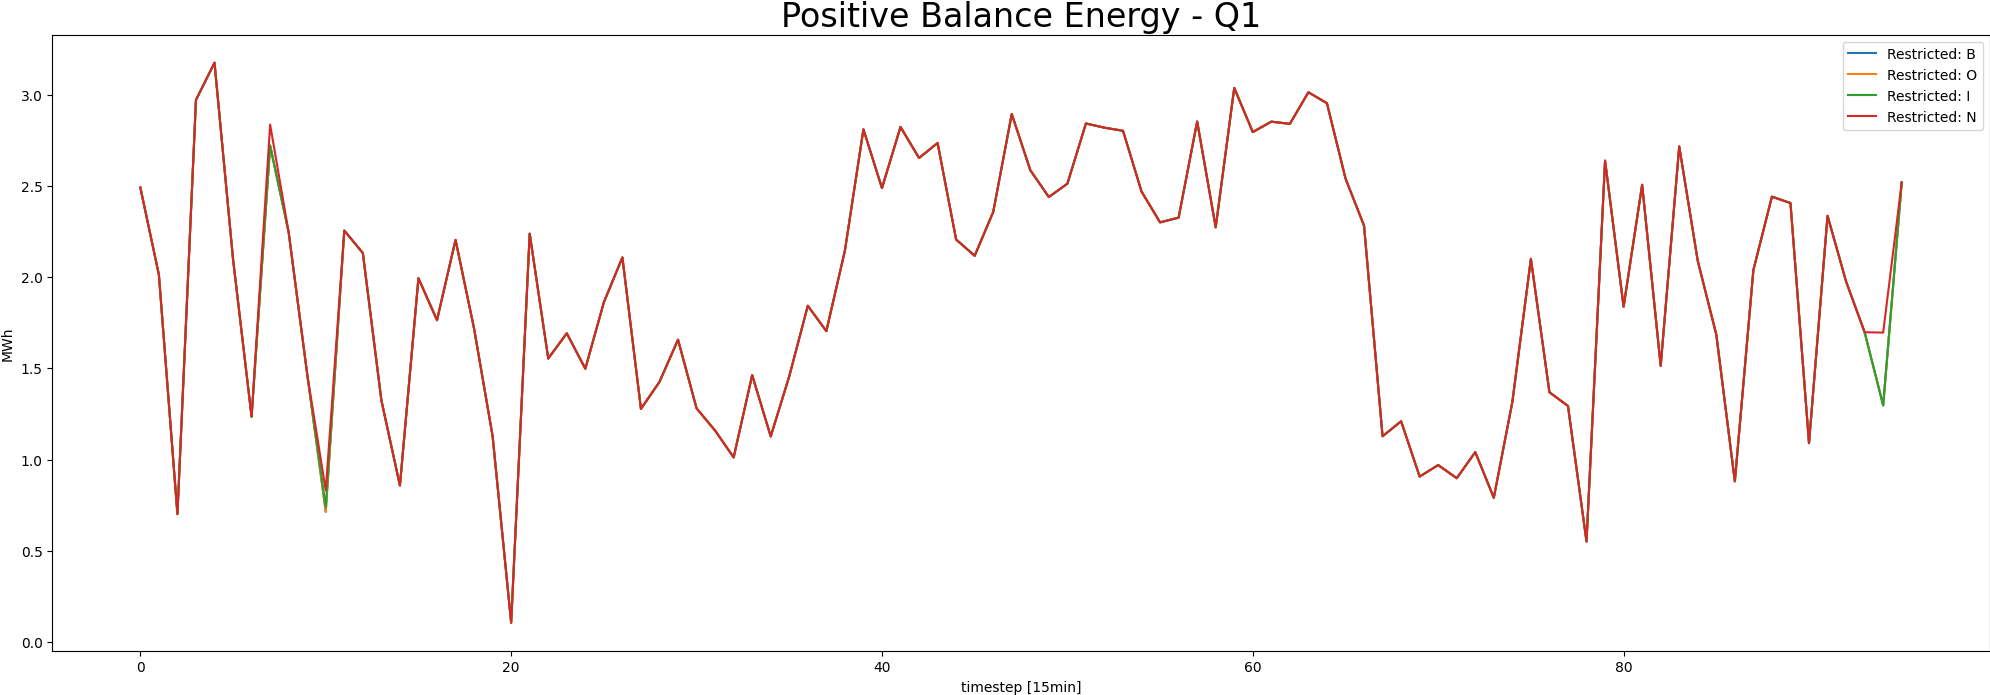
\includegraphics[width=1\linewidth]{pictures/results/Positive Balance Energy - Q1.png}
	\caption{Positive Balance Energy - Q1}
	\label{fig:Positive Balance Energy - Q1}
\end{figure}

\begin{figure}[!h]
	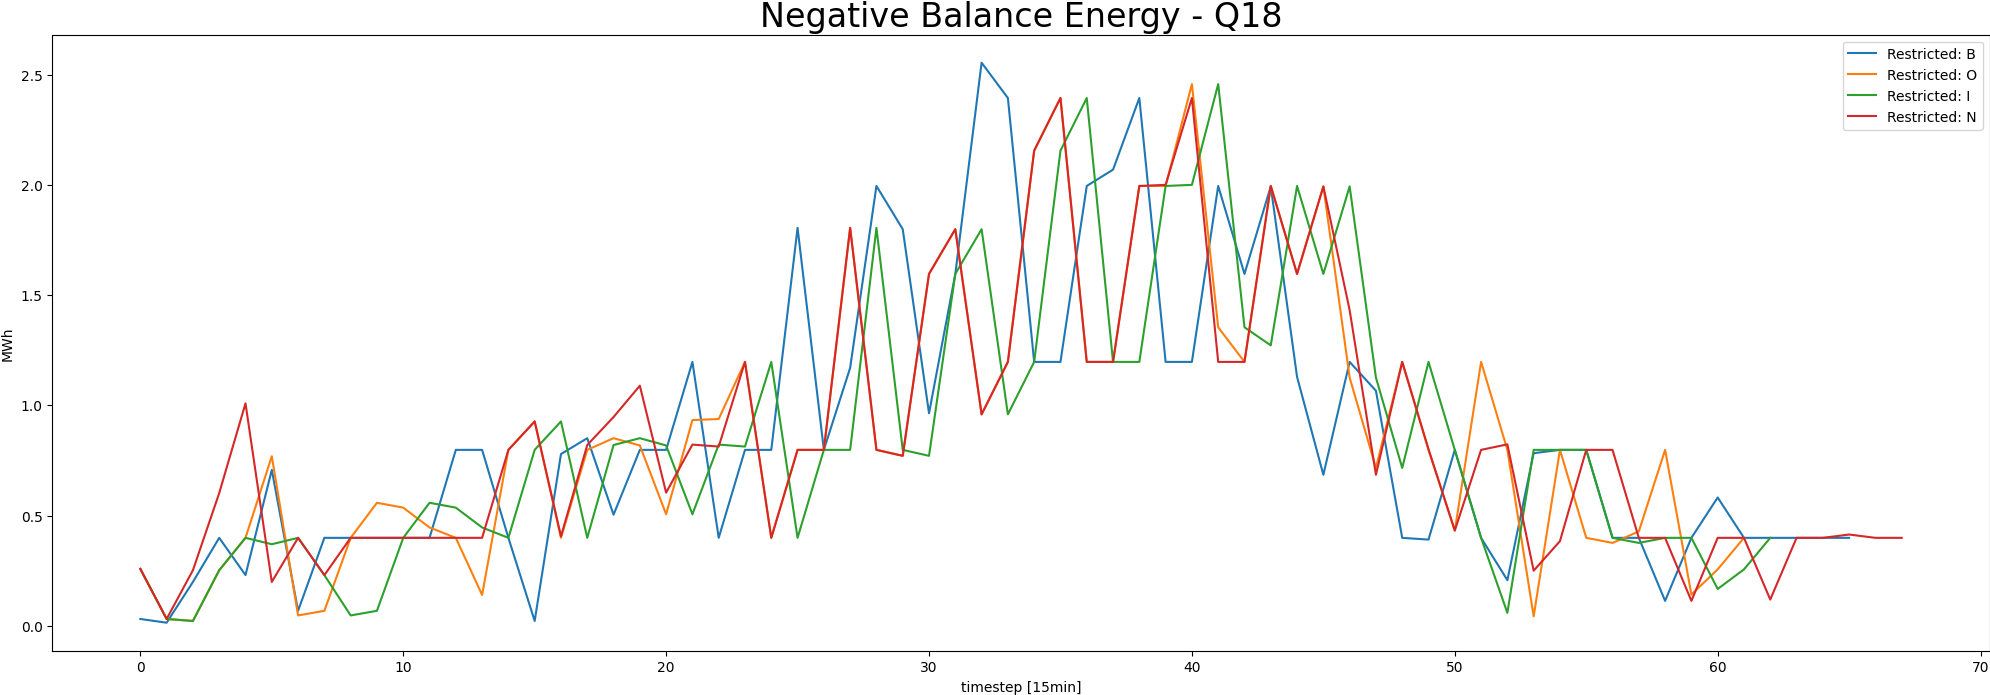
\includegraphics[width=1\linewidth]{pictures/results/Negative Balance Energy - Q18.png}
	\caption{Negative Balance Energy - Q18}
	\label{fig:Negative Balance Energy - Q18}
\end{figure}

\begin{figure}[!h]
	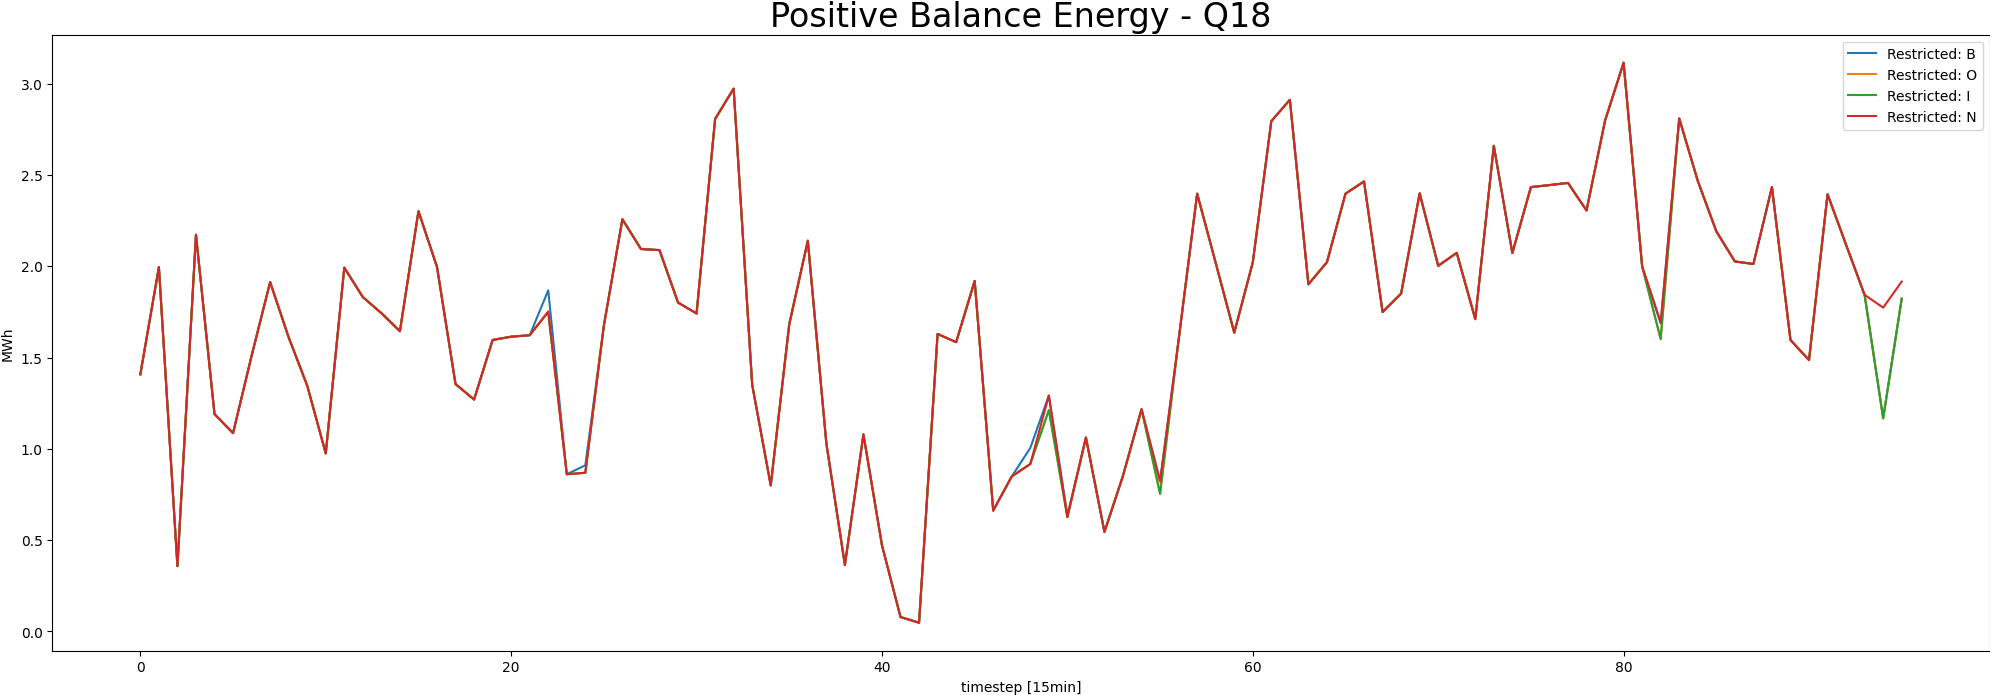
\includegraphics[width=1\linewidth]{pictures/results/Positive Balance Energy - Q18.png}
	\caption{Positive Balance Energy - Q18}
	\label{fig:Positive Balance Energy - Q18}
\end{figure}

\begin{figure}[!h]
	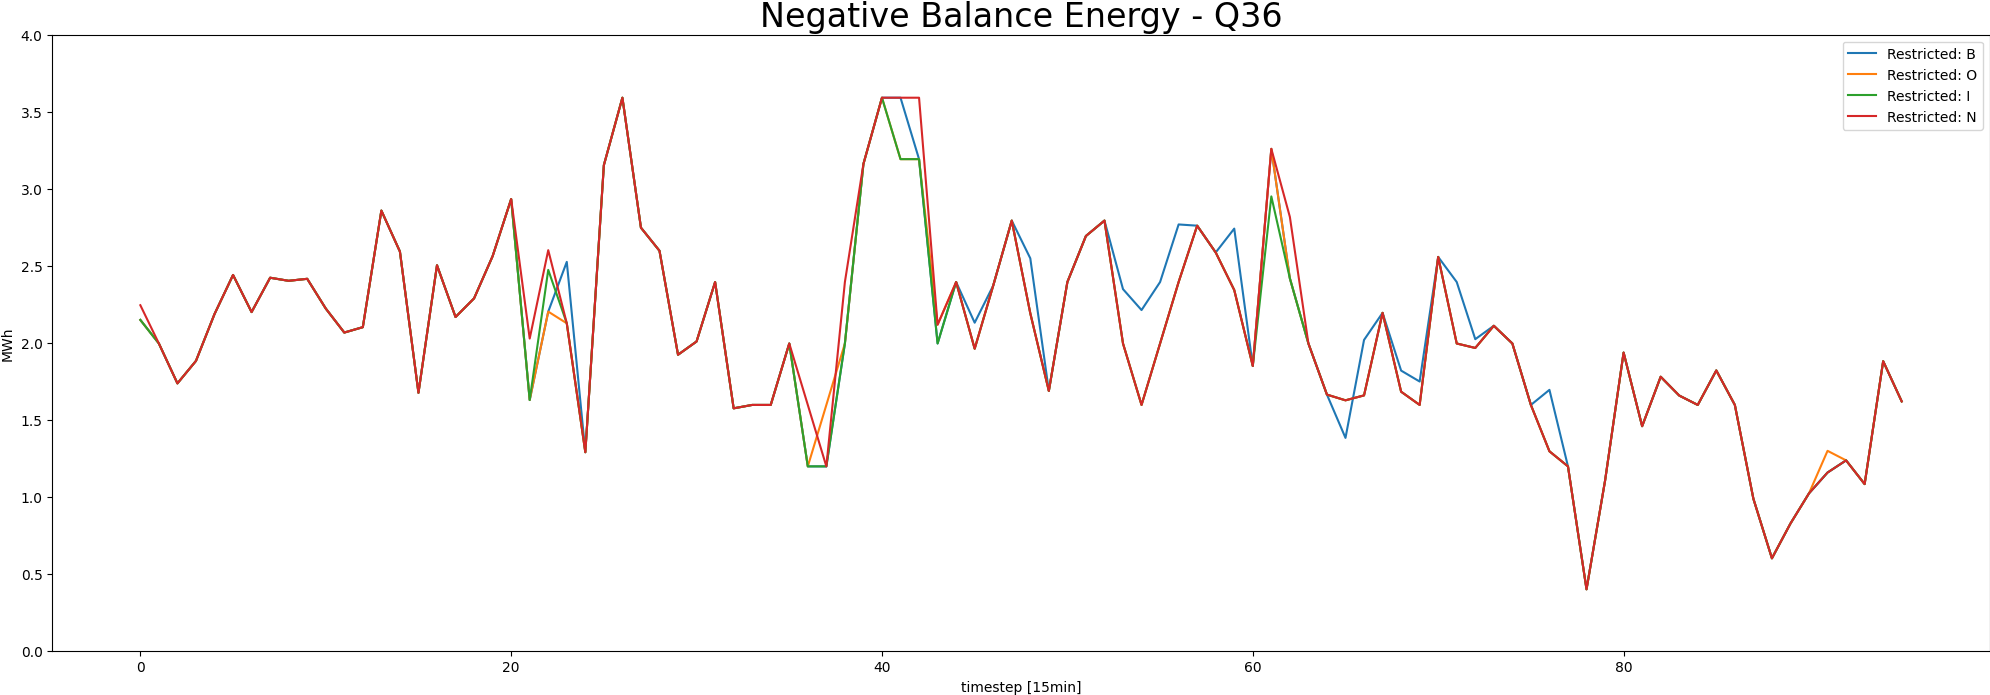
\includegraphics[width=1\linewidth]{pictures/results/Negative Balance Energy - Q36.png}
	\caption{Negative Balance Energy - Q36}
	\label{fig:Negative Balance Energy - Q36}
\end{figure}

\begin{figure}[!h]
	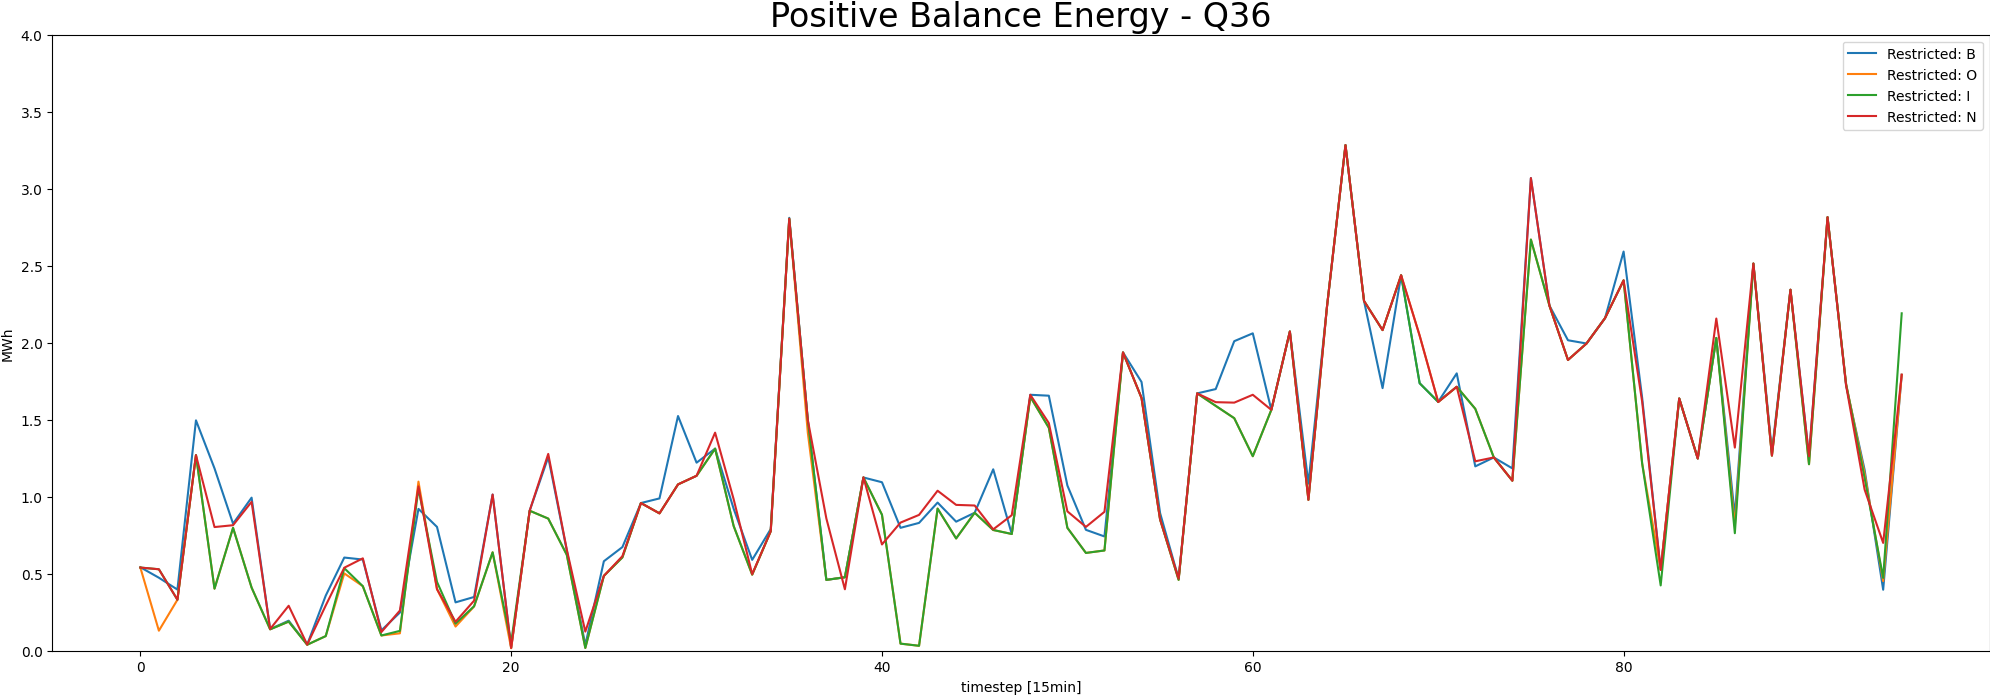
\includegraphics[width=1\linewidth]{pictures/results/Positive Balance Energy - Q36.png}
	\caption{Positive Balance Energy - Q36}
	\label{fig:Positive Balance Energy - Q36}
\end{figure}

\chapter{Conclusion}

$\rightarrow$ This is presumably due to better preparation in scenarios where large fluctuations are expected.\\
$\rightarrow$ Conversely, in scenarios where the majority of providers do not anticipate high volatility, an unexpected surge in demand appears to trigger a **price shock**.\\


aFFR capacity:\\
$\rightarrow$ This suggests that many providers expect to deliver balancing energy the following day.\\
$\rightarrow$ In this context, the balancing energy price serves as a form of "bonus" revenue, which leads to an oversupply—driven by higher participation—that ultimately results in falling prices for balancing energy.\\

aFFR negative energy:\\
$\rightarrow$ This leads to more predictable obligations and a smoother charging curve, while in higher-price scenarios the focus shifts toward capturing price peaks as efficiently as possible.\\
$\rightarrow$ Whether such optimization could be achieved in practice, or only under perfect information in the scenario model, remains uncertain.\\

aFFR capacity:\\
$\rightarrow$ Bids are submitted in such a way that the battery storage system can reliably meet all constraints without significantly impacting the balancing energy market.\\

\todo{hier nochmal rein das die ganze sache am RA markt forecasting hängt, und das man gute erfolge damit haben könnte wenn man nicht probiert bestimmte genaue zahlen zu
	forecasten sondern eher annimmt das der markt bestimmten rythmen unterliegt --> verweiß auf appendix als einen aufschlag dazu}

\todo{ob die aufteilugn in q36 zwischen RA und DA wirklich so geschieht ist stark davon bedingt ob man den RA markt so genau vorhersagen kann
	und damit so perfekt alle preisspitzen mitnehmen kann}
The analyses presented in this work clearly demonstrate that increasing market penetration by volatile energy producers
has significant effects on both the utilization and pricing of balancing energy. In particular,
it is observed that with a growing share of volatile generation, the volume of activated negative balancing energy increases,
while demand for positive balancing energy decreases. This pattern is also reflected in the marginal prices: while the prices
for negative balancing energy tend to rise with increasing generation volatility, the prices for positive balancing energy show
a declining trend.

Notably, strong price outliers can be observed for positive balancing energy in scenarios with low or medium market penetration
by volatile producers. These anomalies appear to be driven by unexpectedly high demand peaks in scenarios where market participants
did not anticipate major fluctuations. This suggests that the expectations and preparedness of market participants play a crucial
role in maintaining price stability under conditions of variable renewable energy feed-in.

The analyzed capacity prices reveal a nuanced picture: median values peak for both positive and negative balancing energy
in the medium scenario, indicating heightened competition in this setting\todo{nochmal überlegen ob das hier sinn macht}.
Furthermore, the lower quantiles reveal that for
negative balancing energy, there is little difference between Q1 and Q36, whereas for positive balancing energy,
a more pronounced price divergence occurs towards the end of the day. This implies that in scenarios with anticipated high volatility,
providers expect to deliver balancing energy the following day and treat the capacity price as an opportunistic “take-along price.”
This behavior leads to a supply increase that exceeds the rise in demand, resulting in falling energy prices.

Across all scenarios, the bidding strategies for the balancing capacity market are positioned just below the expected marginal prices.

In scenarios with low to medium levels of volatile production, a shift toward earlier provisioning in the negative balancing energy
market is observed. This is reflected in a more regular schedule of negative balancing energy delivery. In contrast, in high volatility
scenarios with elevated prices, a strategy focused on capitalizing on price peaks becomes evident. In such cases, providers may forgo
profits in the capacity market in favor of maximizing returns in the energy market.

In the domain of negative balancing energy in particular, earlier provisioning is evident in scenarios with low and medium price levels.
This suggests stronger adherence to obligations and more regular charging patterns. By contrast, in high-price scenarios, the focus shifts towards optimal exploitation of price spikes—a strategy that may not be fully replicable under real market conditions, as it presumes perfect knowledge of future price developments.

For positive balancing energy, the analysis reveals that bidding volumes in low and medium volatility scenarios differ only marginally.
Pronounced differences emerge only in high-volatility scenarios. Again, the data show that the more restrictive the capacity market
constraints, the earlier the provision of balancing energy occurs.

Overall, the findings highlight that both the expectations of market participants and their bidding strategies in the aFFR capacity and
energy balancing markets play a critical role in price formation.

It is also worth noting that, while the model accounts for different possible aFFR energy market scenarios,
it assumes perfect foresight within each individual daily scenario.
As a result, the revenue potential from the aFFR energy market is likely overestimated.
Moreover, the model heavily exploits price peaks, which may not be fully realizable in practice.
Whether such behavior can be implemented in reality depends largely on the quality of intraday forecasts
and requires further investigation.

An alternative modeling approach would be to refrain from using precise price data for the aFFR energy market
and instead attempt to represent general market cycles.
Under the hypothesis that the transmission system operator continuously strives to balance the grid,
it can be postulated that any imbalance will eventually be corrected.
Prolonged imbalances are assumed to be relatively unlikely.
Based on this assumption, certain recurring patterns could be forecasted within a 4-hour window,
characterized by a defined expected value.
Appendix \ref{app:altModel} presents a preliminary model approach for this idea.
However, both the scientific validation of the underlying hypothesis and the development of a suitable aFFR prediction cycle algorithm
remain subjects for further research.



\begin{enumerate}
	\item Only a single day was simulated; the actual reload effects may become relevant only in multi-day scenarios.
\end{enumerate}

\todo{Include simulations with other providers}

\todo{evenutell noch mit rein das die optimierung der windkraft noch komplett fehlt so kann die batterie auch genutzt werden
	um relativ teure fehler aus zu gleichen wie im paper (Optimal Dispatch Scheduling of a Wind-Battery-System in German
	Power Market) opmitiert}


%% ********************
%% Backmatter
%% ********************
%\backmatter

\chapter{Appendix}
%% change chapter title to german if necessary
%% *** local page settings ***
\markright{Appendix}
\addtocontents{toc}{\protect\setcounter{tocdepth}{-1}} %decrease the depth of the appendix entry in the ToC
\setcounter{table}{0}
\setcounter{figure}{0}
\renewcommand{\thefigure}{A.\arabic{figure}}
\renewcommand{\thetable}{A.\arabic{table}}


\section{Further Model Constraints}

\begin{flalign}
	\label{parkCon_Q^{rB}_{DA}(t_{hour})}                   \sum((s_DA, s^{in}_{RL}, s^{out}_{RL}), Q^{rB}_{DA}(t_{hour}, s^{in}_{RL}, s^{out}_{RL})) \leq parkCap * parkProfile(t_{hour}) - \sum((s_DA, s^{in}_{RL}, s^{out}_{RL}), Q_rB_reload(t_{hour}, s^{in}_{RL}, s^{out}_{RL}));
\end{flalign}
\begin{flalign}
	\label{parkCon_Q^{rI}_{DA}(t_{hour})}                   \sum((s_DA, s^{in}_{RL}, s^{out}_{RL}), Q^{rI}_{DA}(t_{hour}, s^{in}_{RL}, s^{out}_{RL})) \leq parkCap * parkProfile(t_{hour}) - \sum((s_DA, s^{in}_{RL}, s^{out}_{RL}), Q_rI_reload(t_{hour}, s^{in}_{RL}, s^{out}_{RL}));
\end{flalign}
\begin{flalign}
	\label{parkCon_Q^{rO}_{DA}(t_{hour})}                   \sum((s_DA, s^{in}_{RL}, s^{out}_{RL}), Q^{rO}_{DA}(t_{hour}, s^{in}_{RL}, s^{out}_{RL})) \leq parkCap * parkProfile(t_{hour}) - \sum((s_DA, s^{in}_{RL}, s^{out}_{RL}), Q_rO_reload(t_{hour}, s^{in}_{RL}, s^{out}_{RL}));
\end{flalign}
\begin{flalign}
	\label{parkCon_Q^{rN}_{DA}(t_{hour})}                   \sum((s_DA, s^{in}_{RL}, s^{out}_{RL}), Q^{rN}_{DA}(t_{hour}, s^{in}_{RL}, s^{out}_{RL})) \leq parkCap * parkProfile(t_{hour}) - \sum((s_DA, s^{in}_{RL}, s^{out}_{RL}), Q_rN_reload(t_{hour}, s^{in}_{RL}, s^{out}_{RL}));
\end{flalign}
\section{Quantile Market Data}

\begin{figure}[!h]
	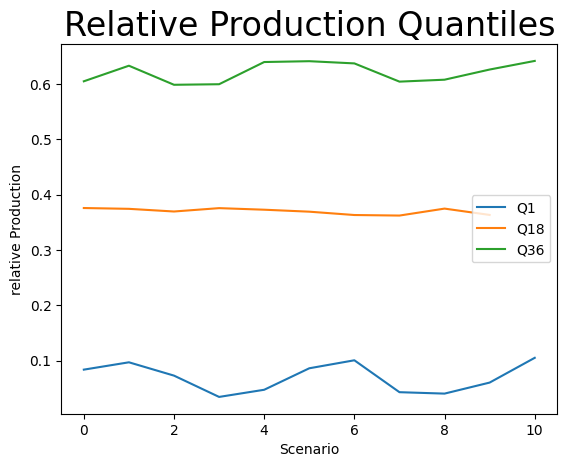
\includegraphics[width=0.7\linewidth]{pictures/results/relativeProduktionQuantils.png}
	\caption{Relative Production Quantiles}
	\label{fig:Relative Production Quantiles}
\end{figure}

Die daraus Resultierenden Zeitreihen für aktivierte Regelarbeit und deren Preise stellen sich dann wie folgt dar:
\begin{figure}[H]
	\centering

	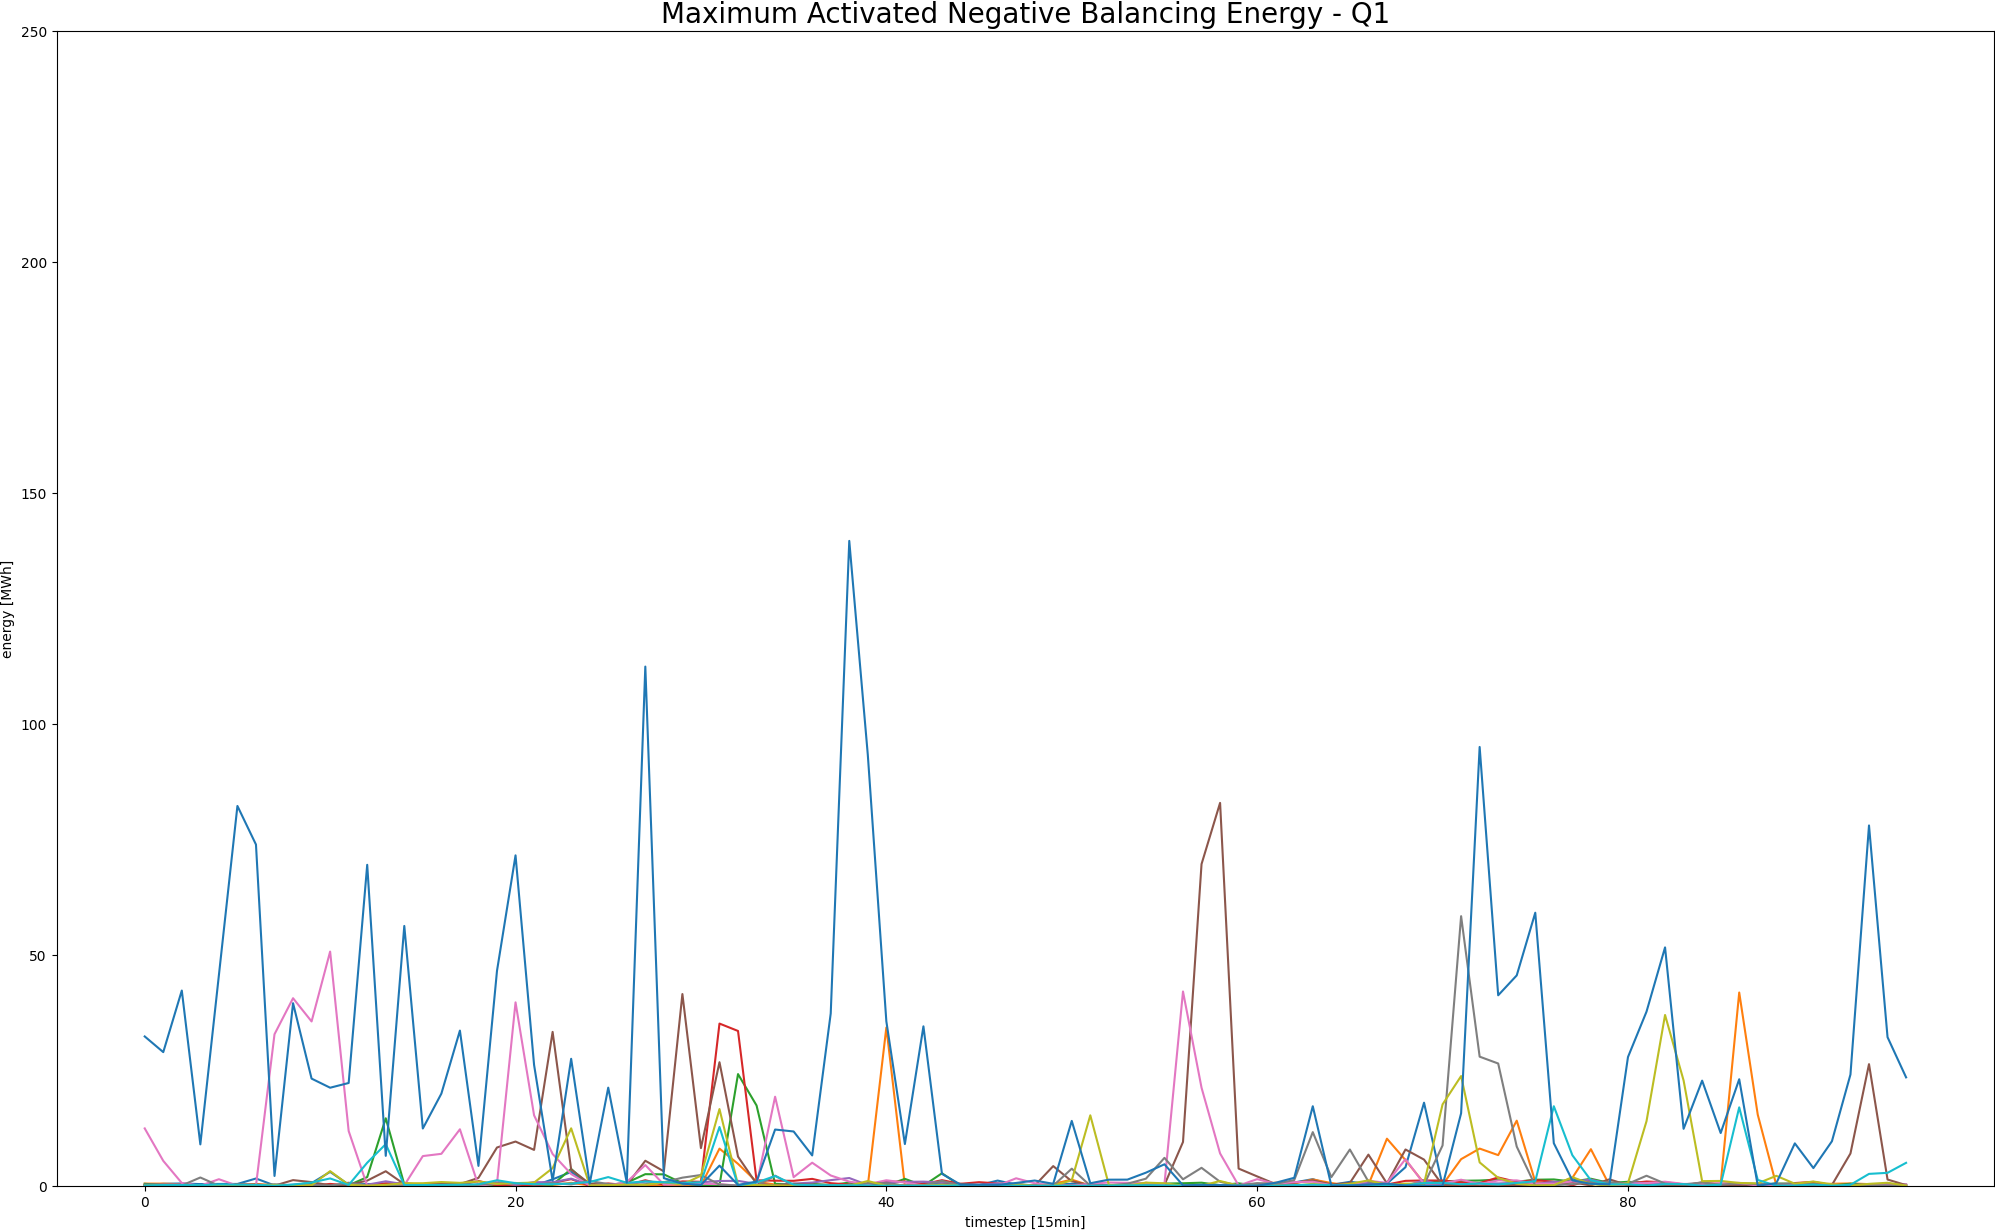
\includegraphics[width=1\linewidth]{pictures/results/Activated_negEnergy_Q1.png}
	\caption{Activated Negative Energy Q1}
	\label{fig:_negEnergy_Q1}
\end{figure}


\begin{figure}[H]
	\centering
	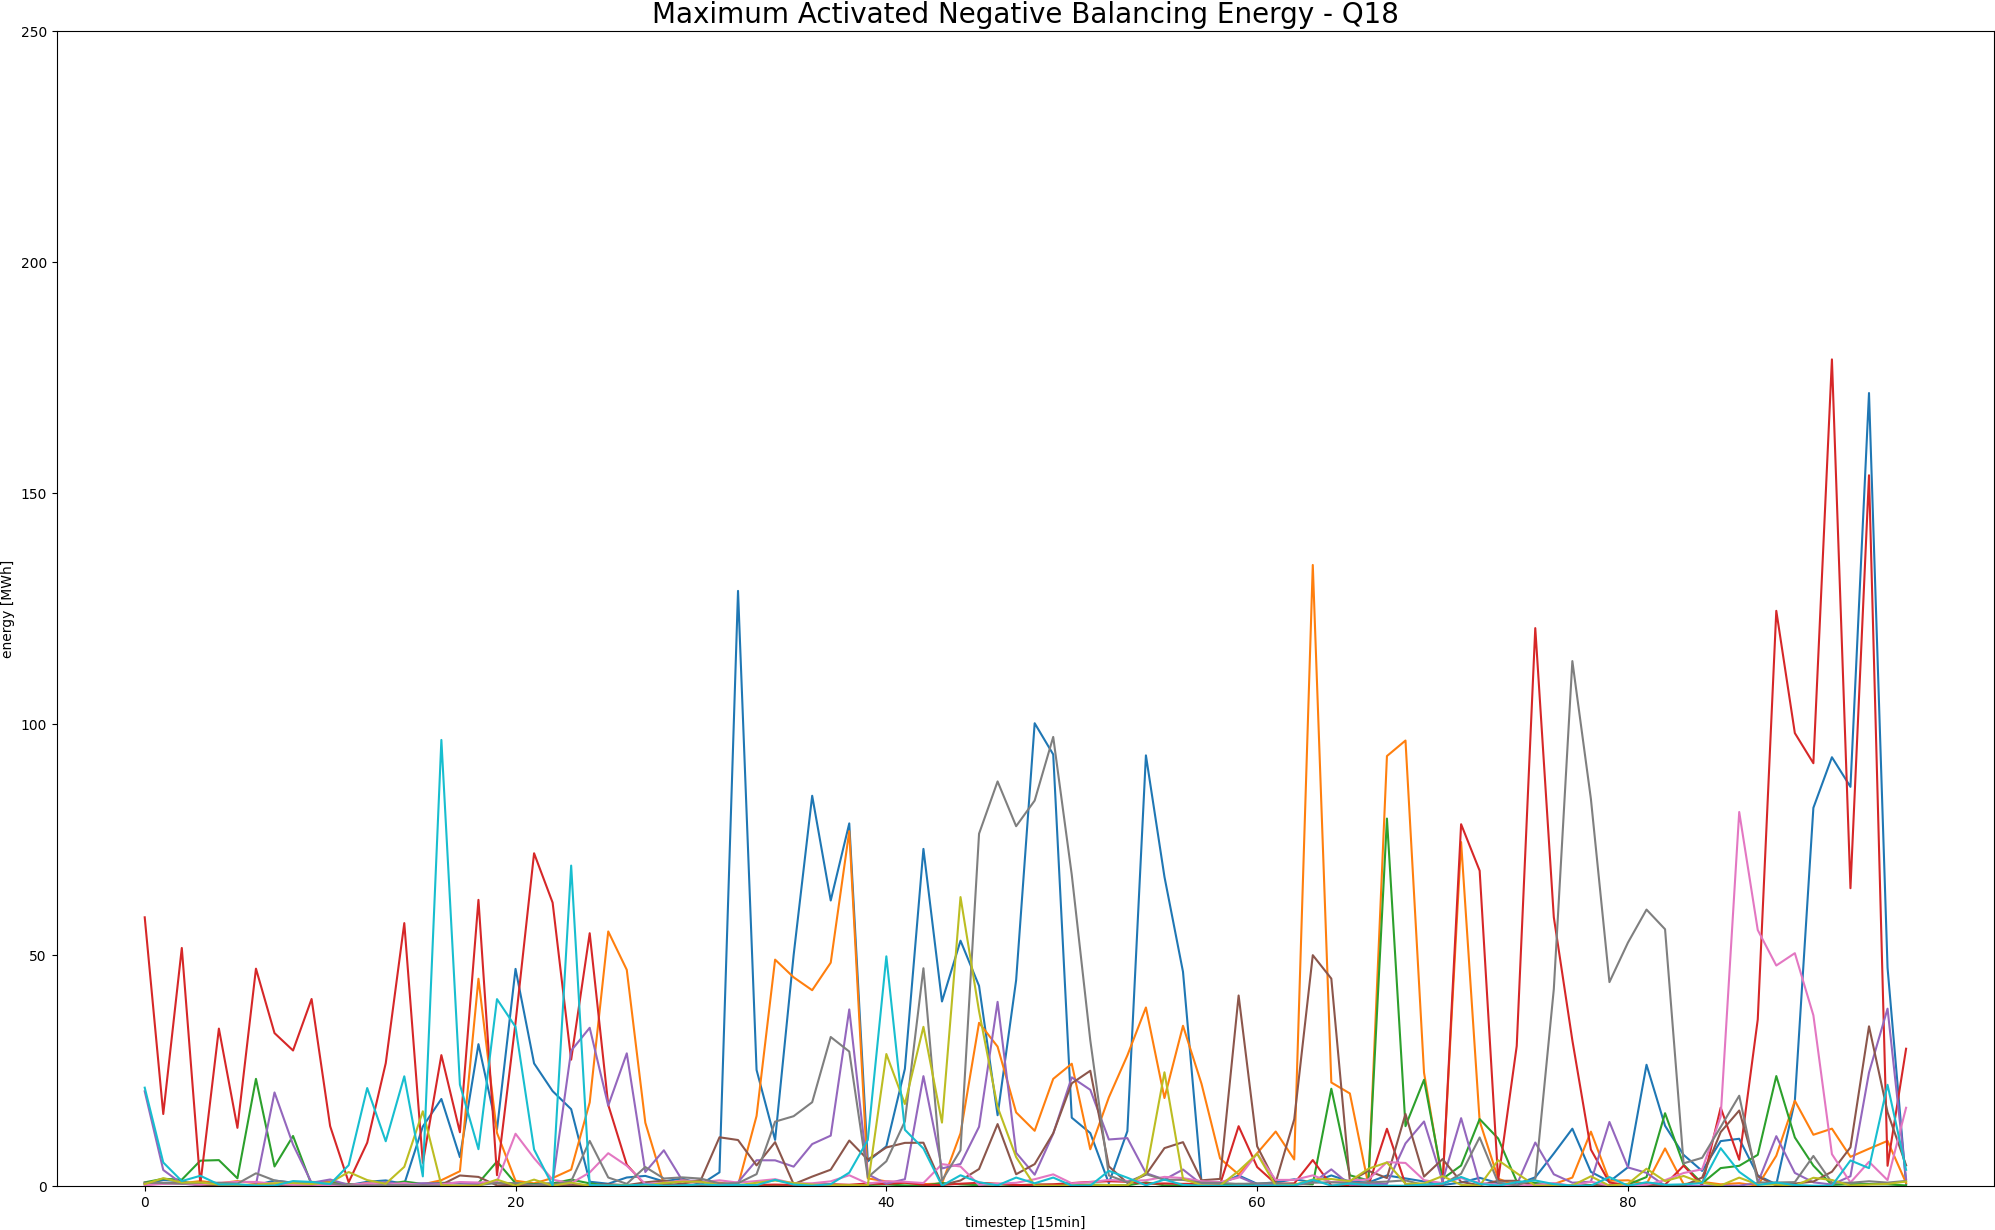
\includegraphics[width=1\linewidth]{pictures/results/Activated_negEnergy_Q18.png}
	\caption{Activated Negative Energy Q18}
	\label{fig:_negEnergy_Q18}
\end{figure}

\begin{figure}[H]
	\centering
	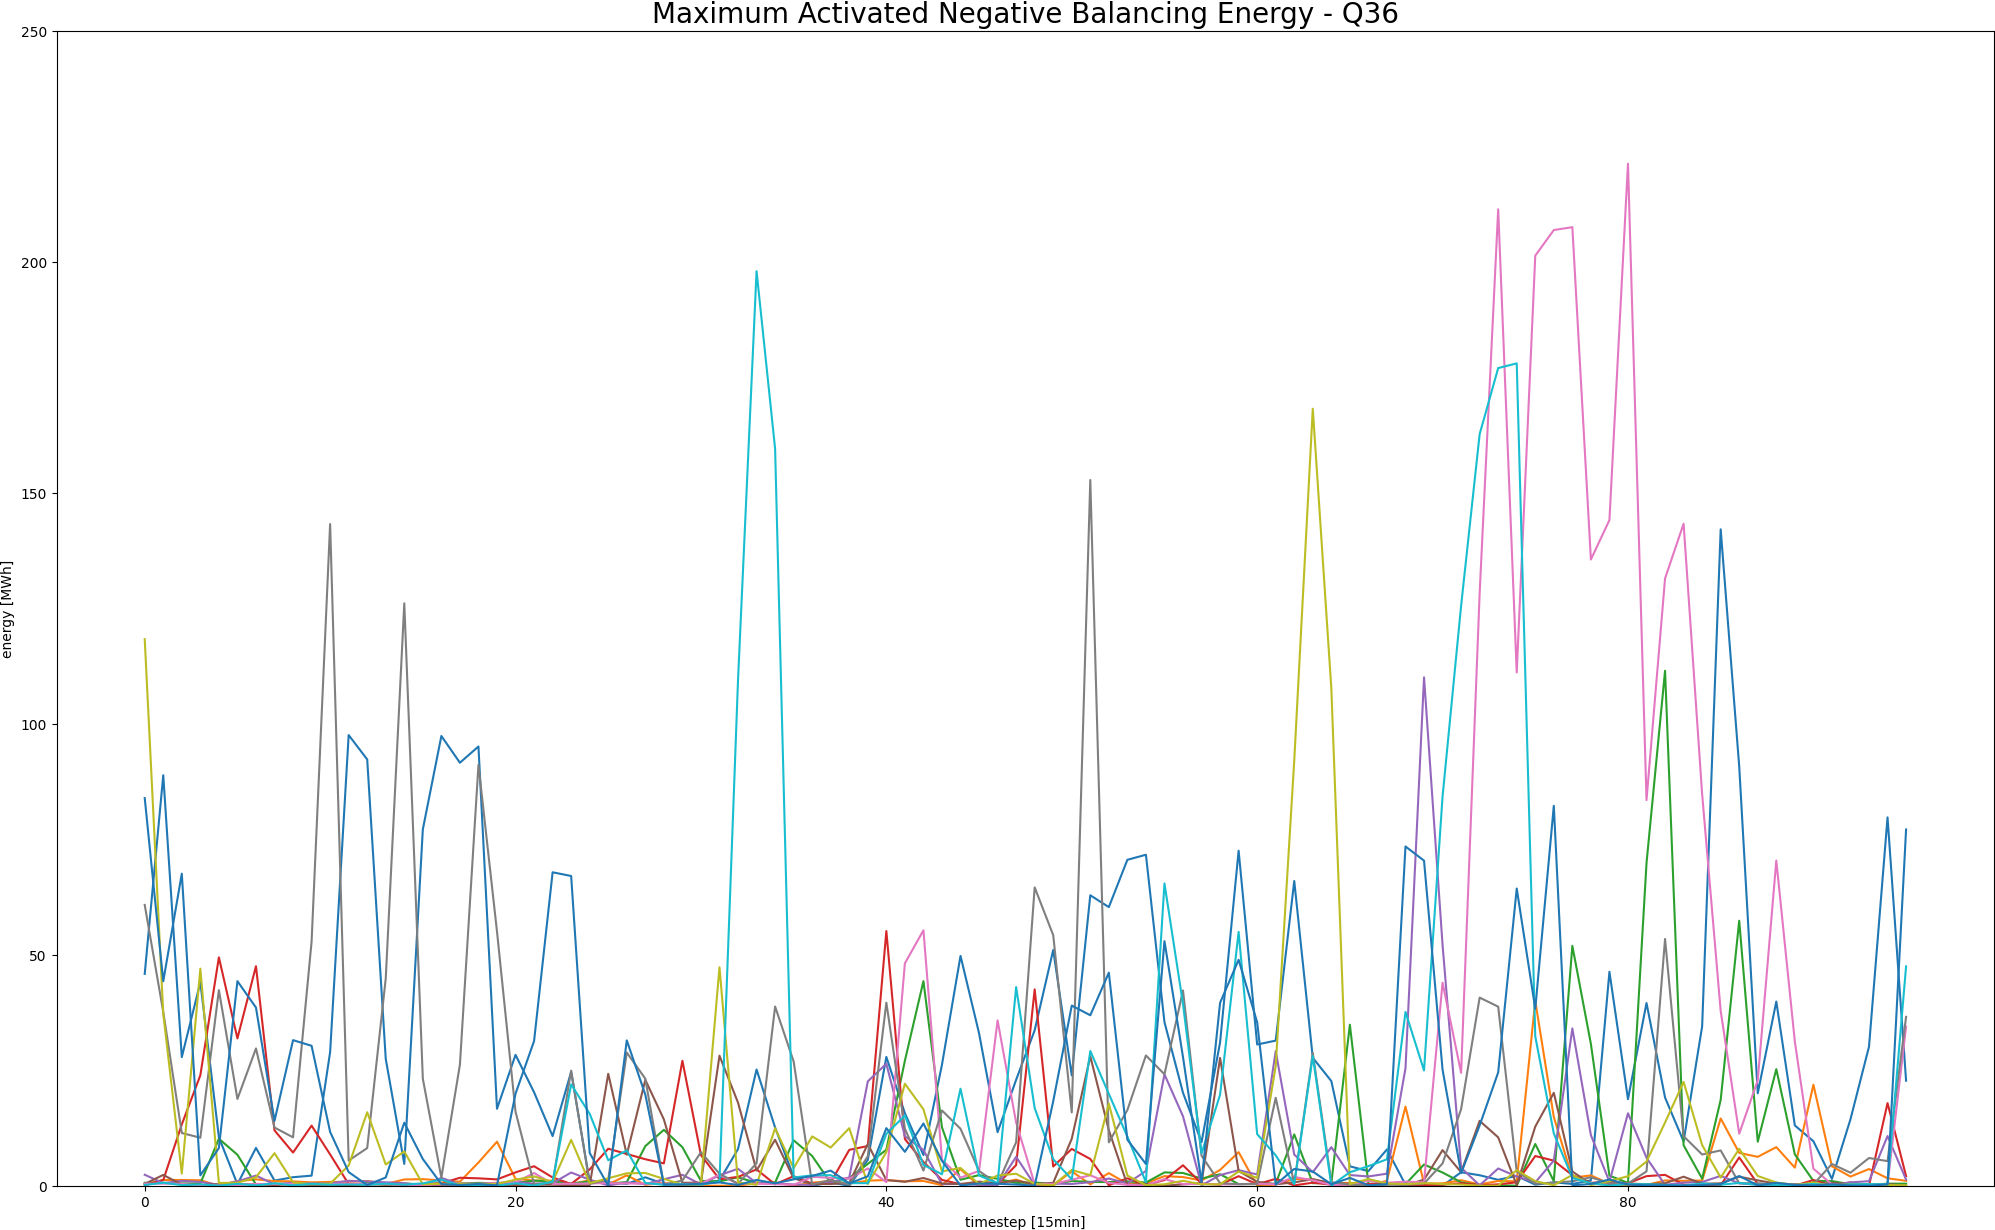
\includegraphics[width=1\linewidth]{pictures/results/Activated_negEnergy_Q36.png}
	\caption{Activated Negative Energy Q36}
	\label{fig:_negEnergy_Q36}
\end{figure}
\begin{figure}
	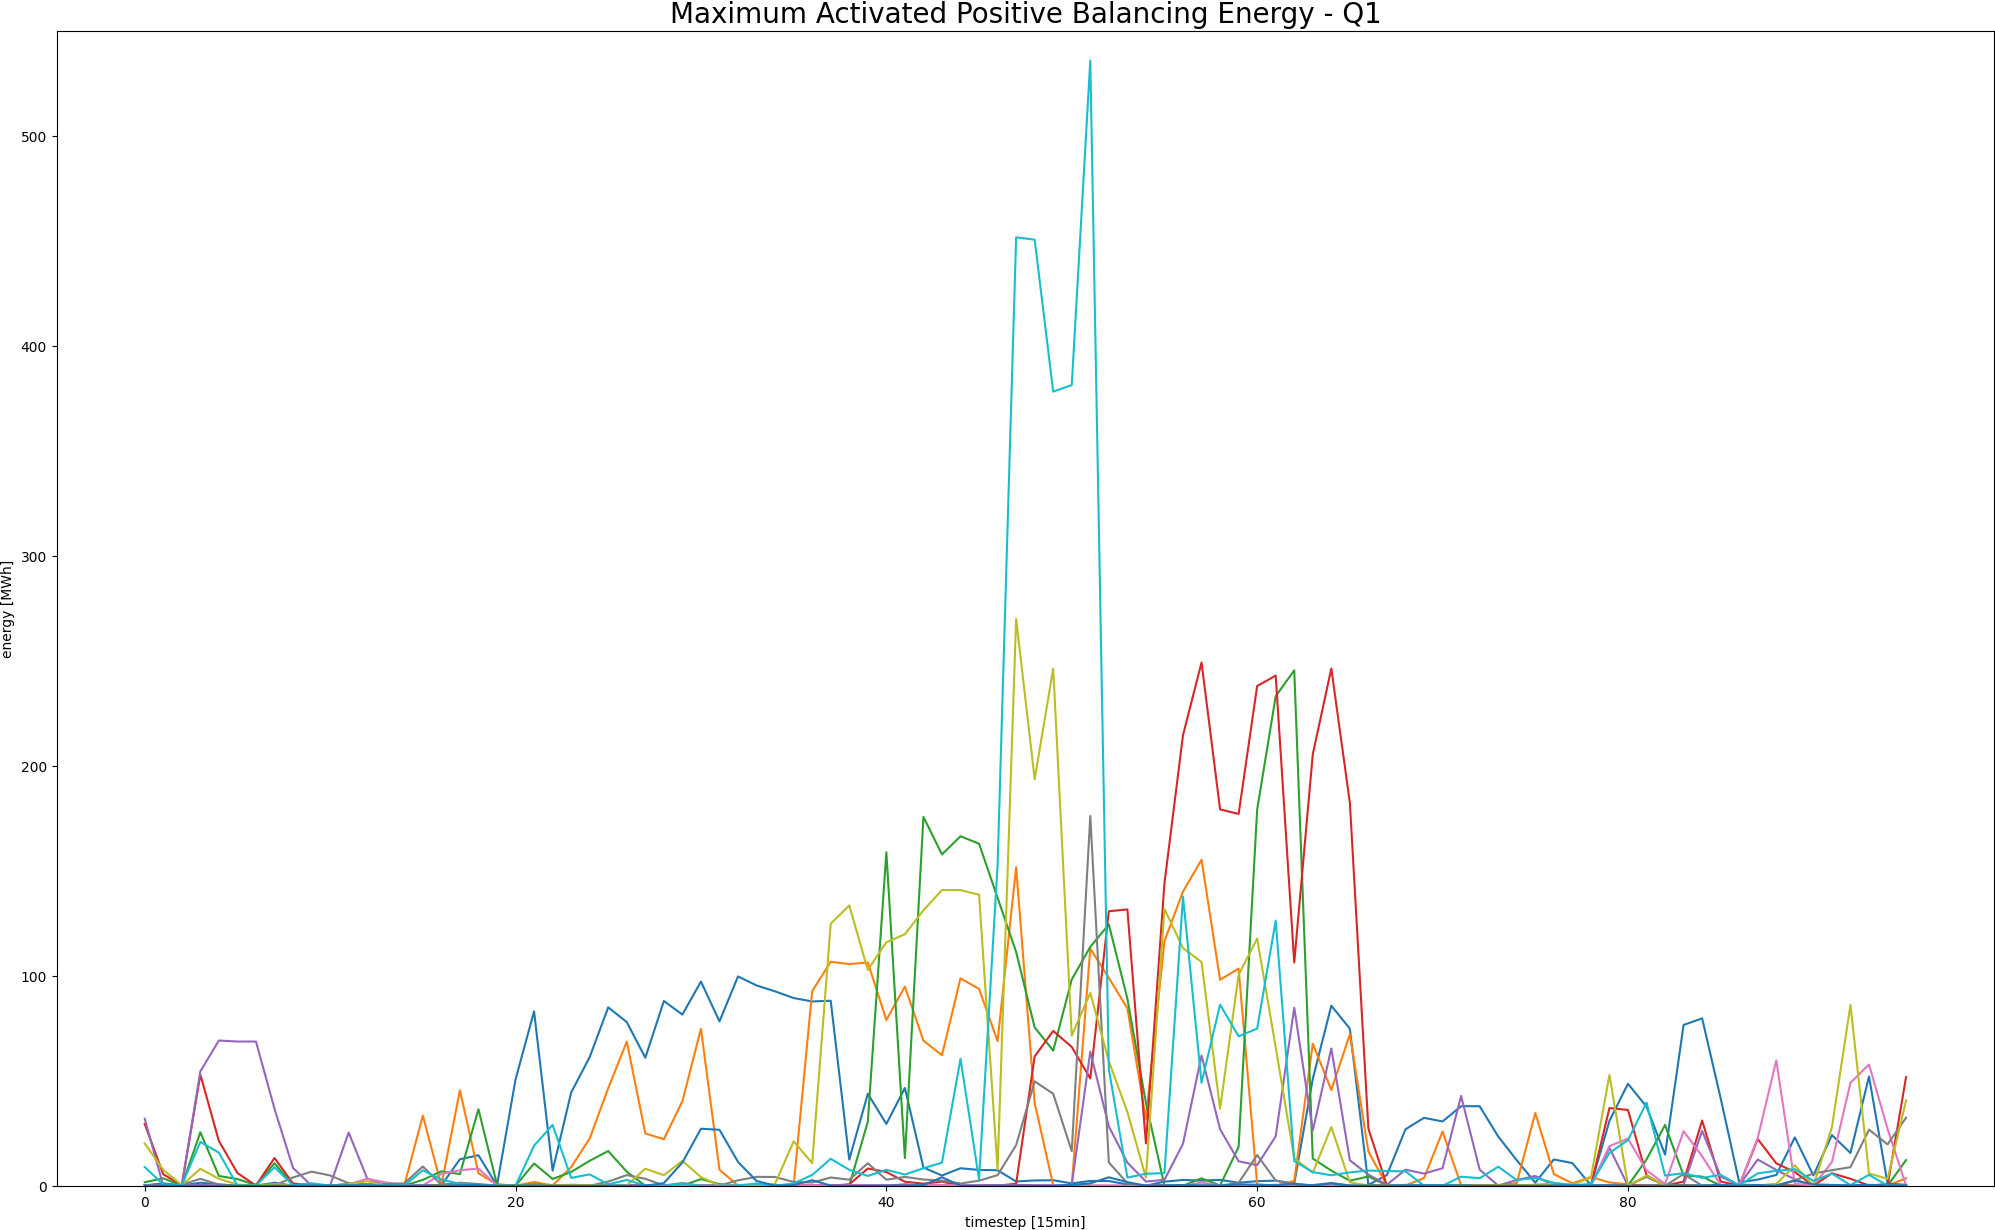
\includegraphics[width=1\linewidth]{pictures/results/Activated_posEnergy_Q1.png}
	\caption{Activated Positive Energy Q1}
	\label{fig:_posEnergy_Q1}
\end{figure}

\begin{figure}
	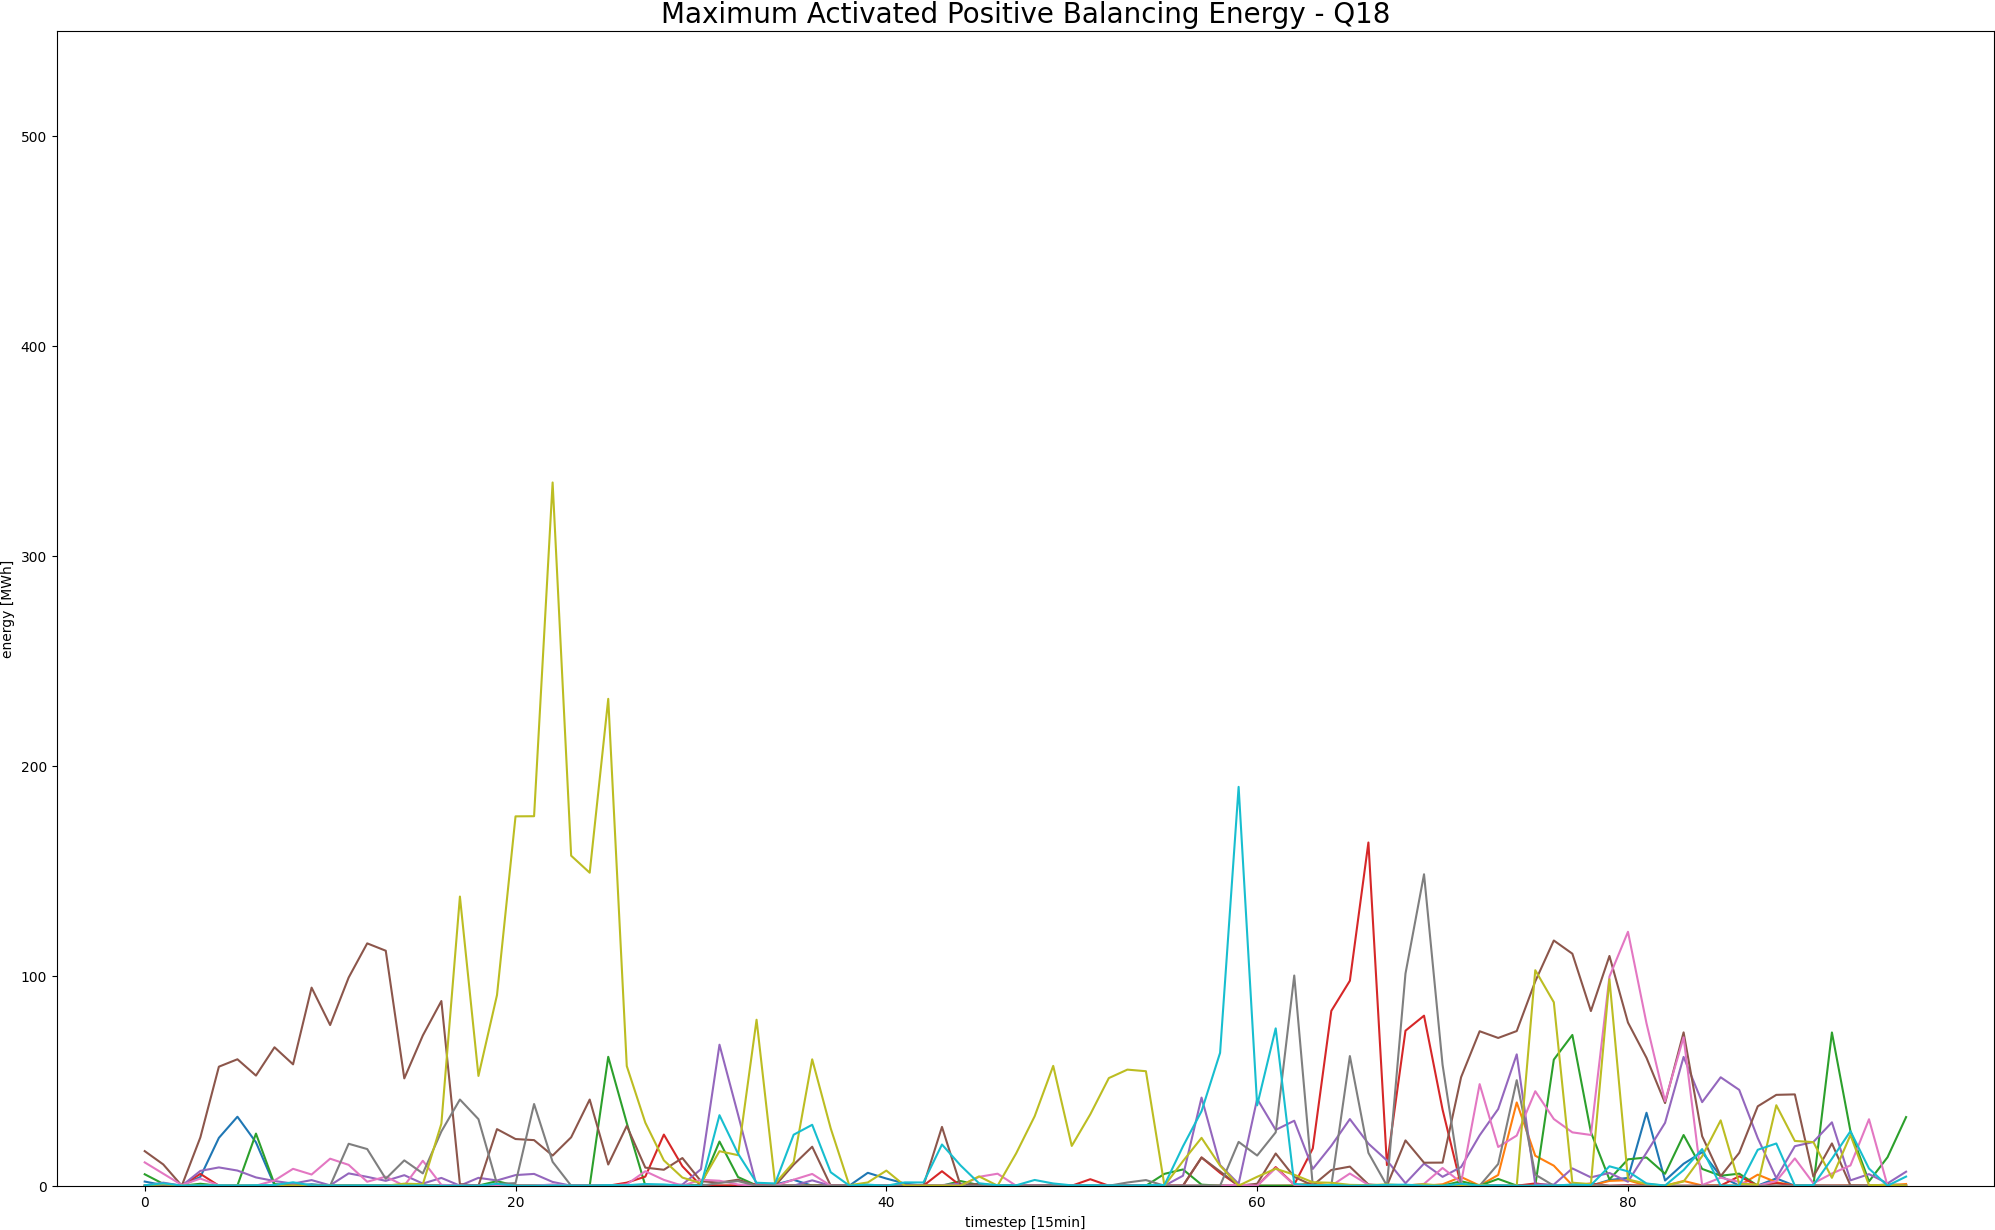
\includegraphics[width=1\linewidth]{pictures/results/Activated_posEnergy_Q18.png}
	\caption{Activated Positive Energy Q18}
	\label{fig:_posEnergy_Q18}
\end{figure}

\begin{figure}
	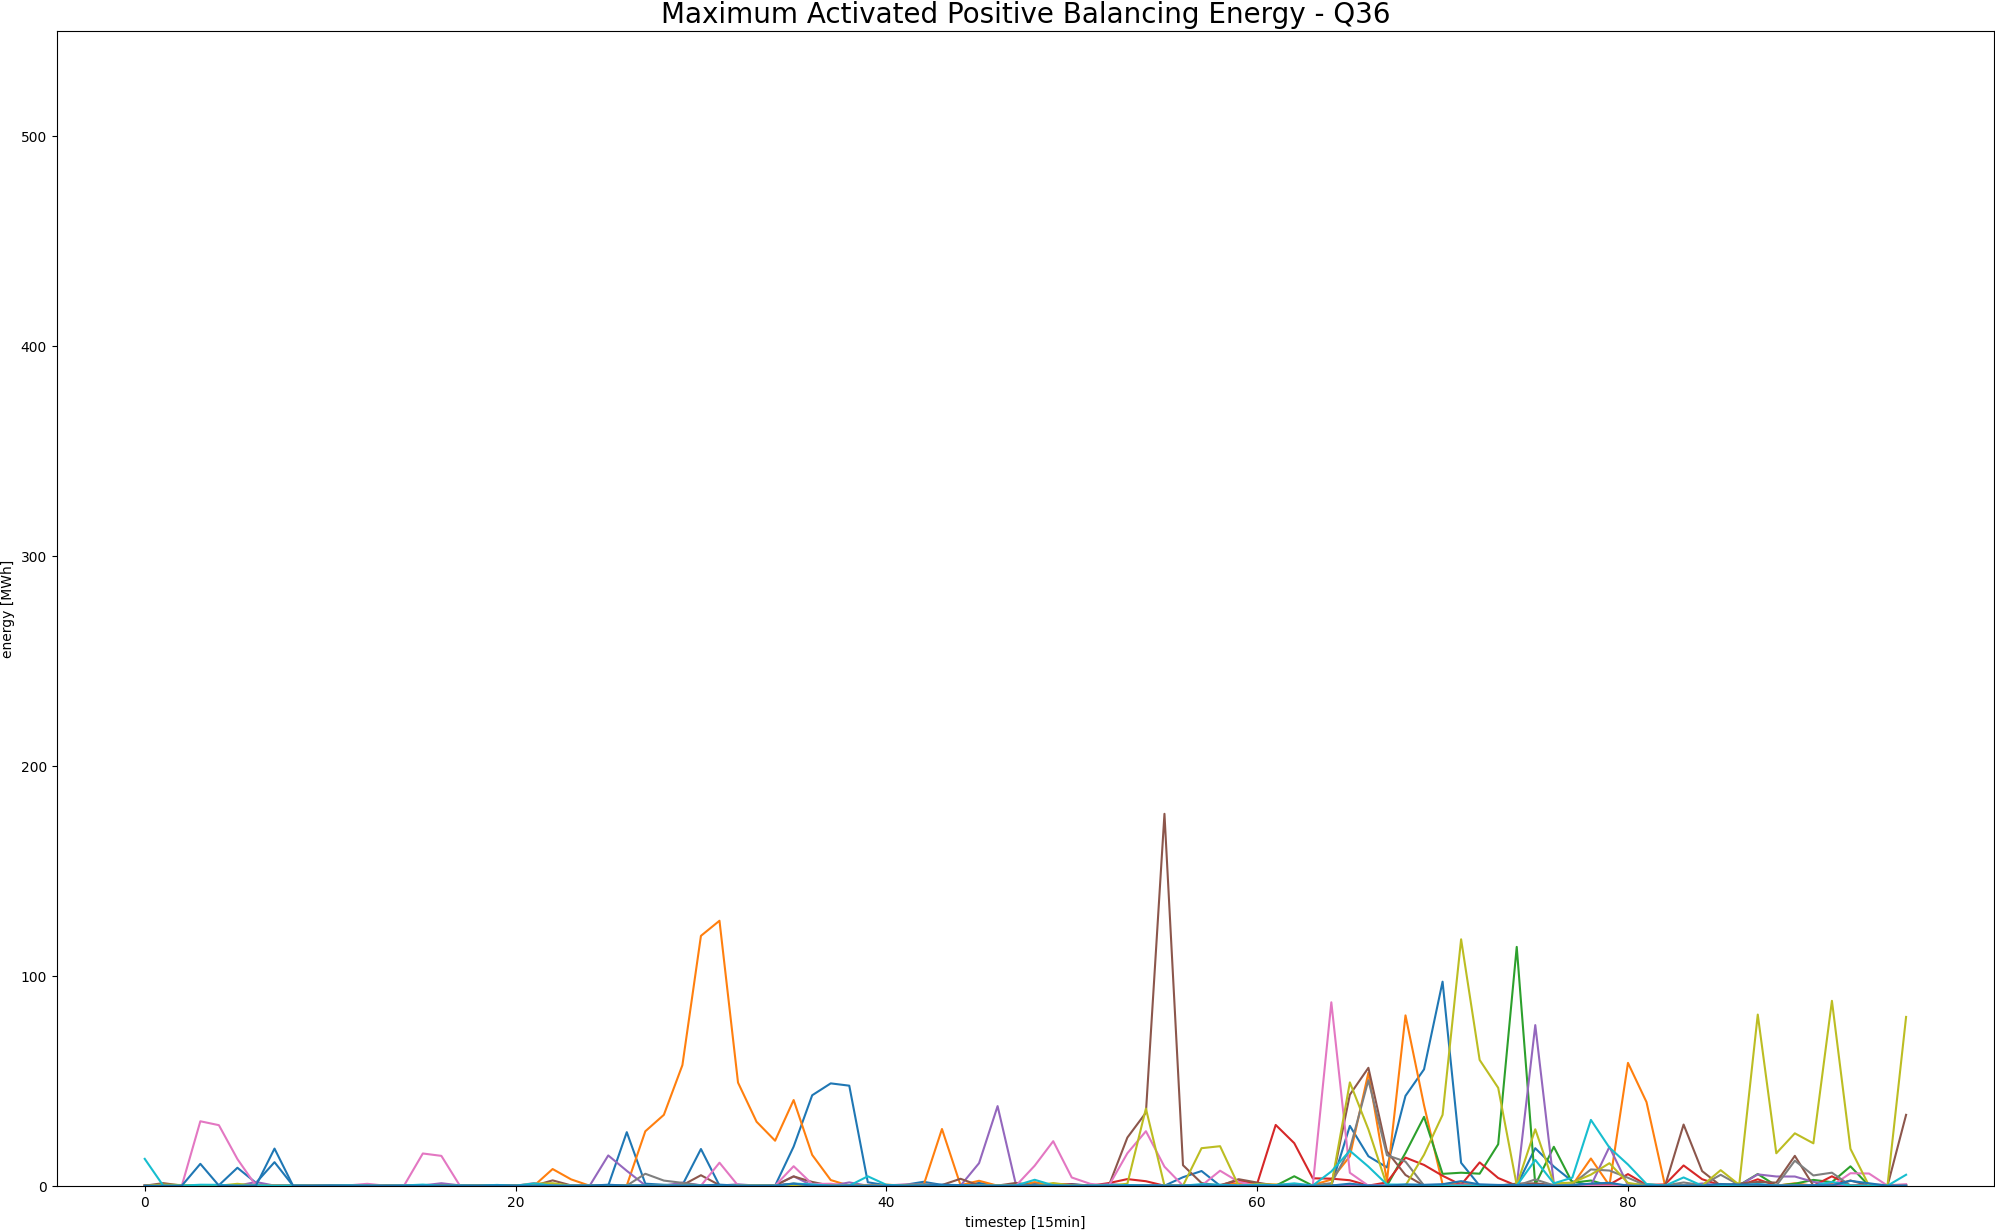
\includegraphics[width=1\linewidth]{pictures/results/Activated_posEnergy_Q36.png}
	\caption{Activated Positive Energy Q36}
	\label{fig:_posEnergy_Q36}
\end{figure}



\begin{figure}[H]
	\centering
	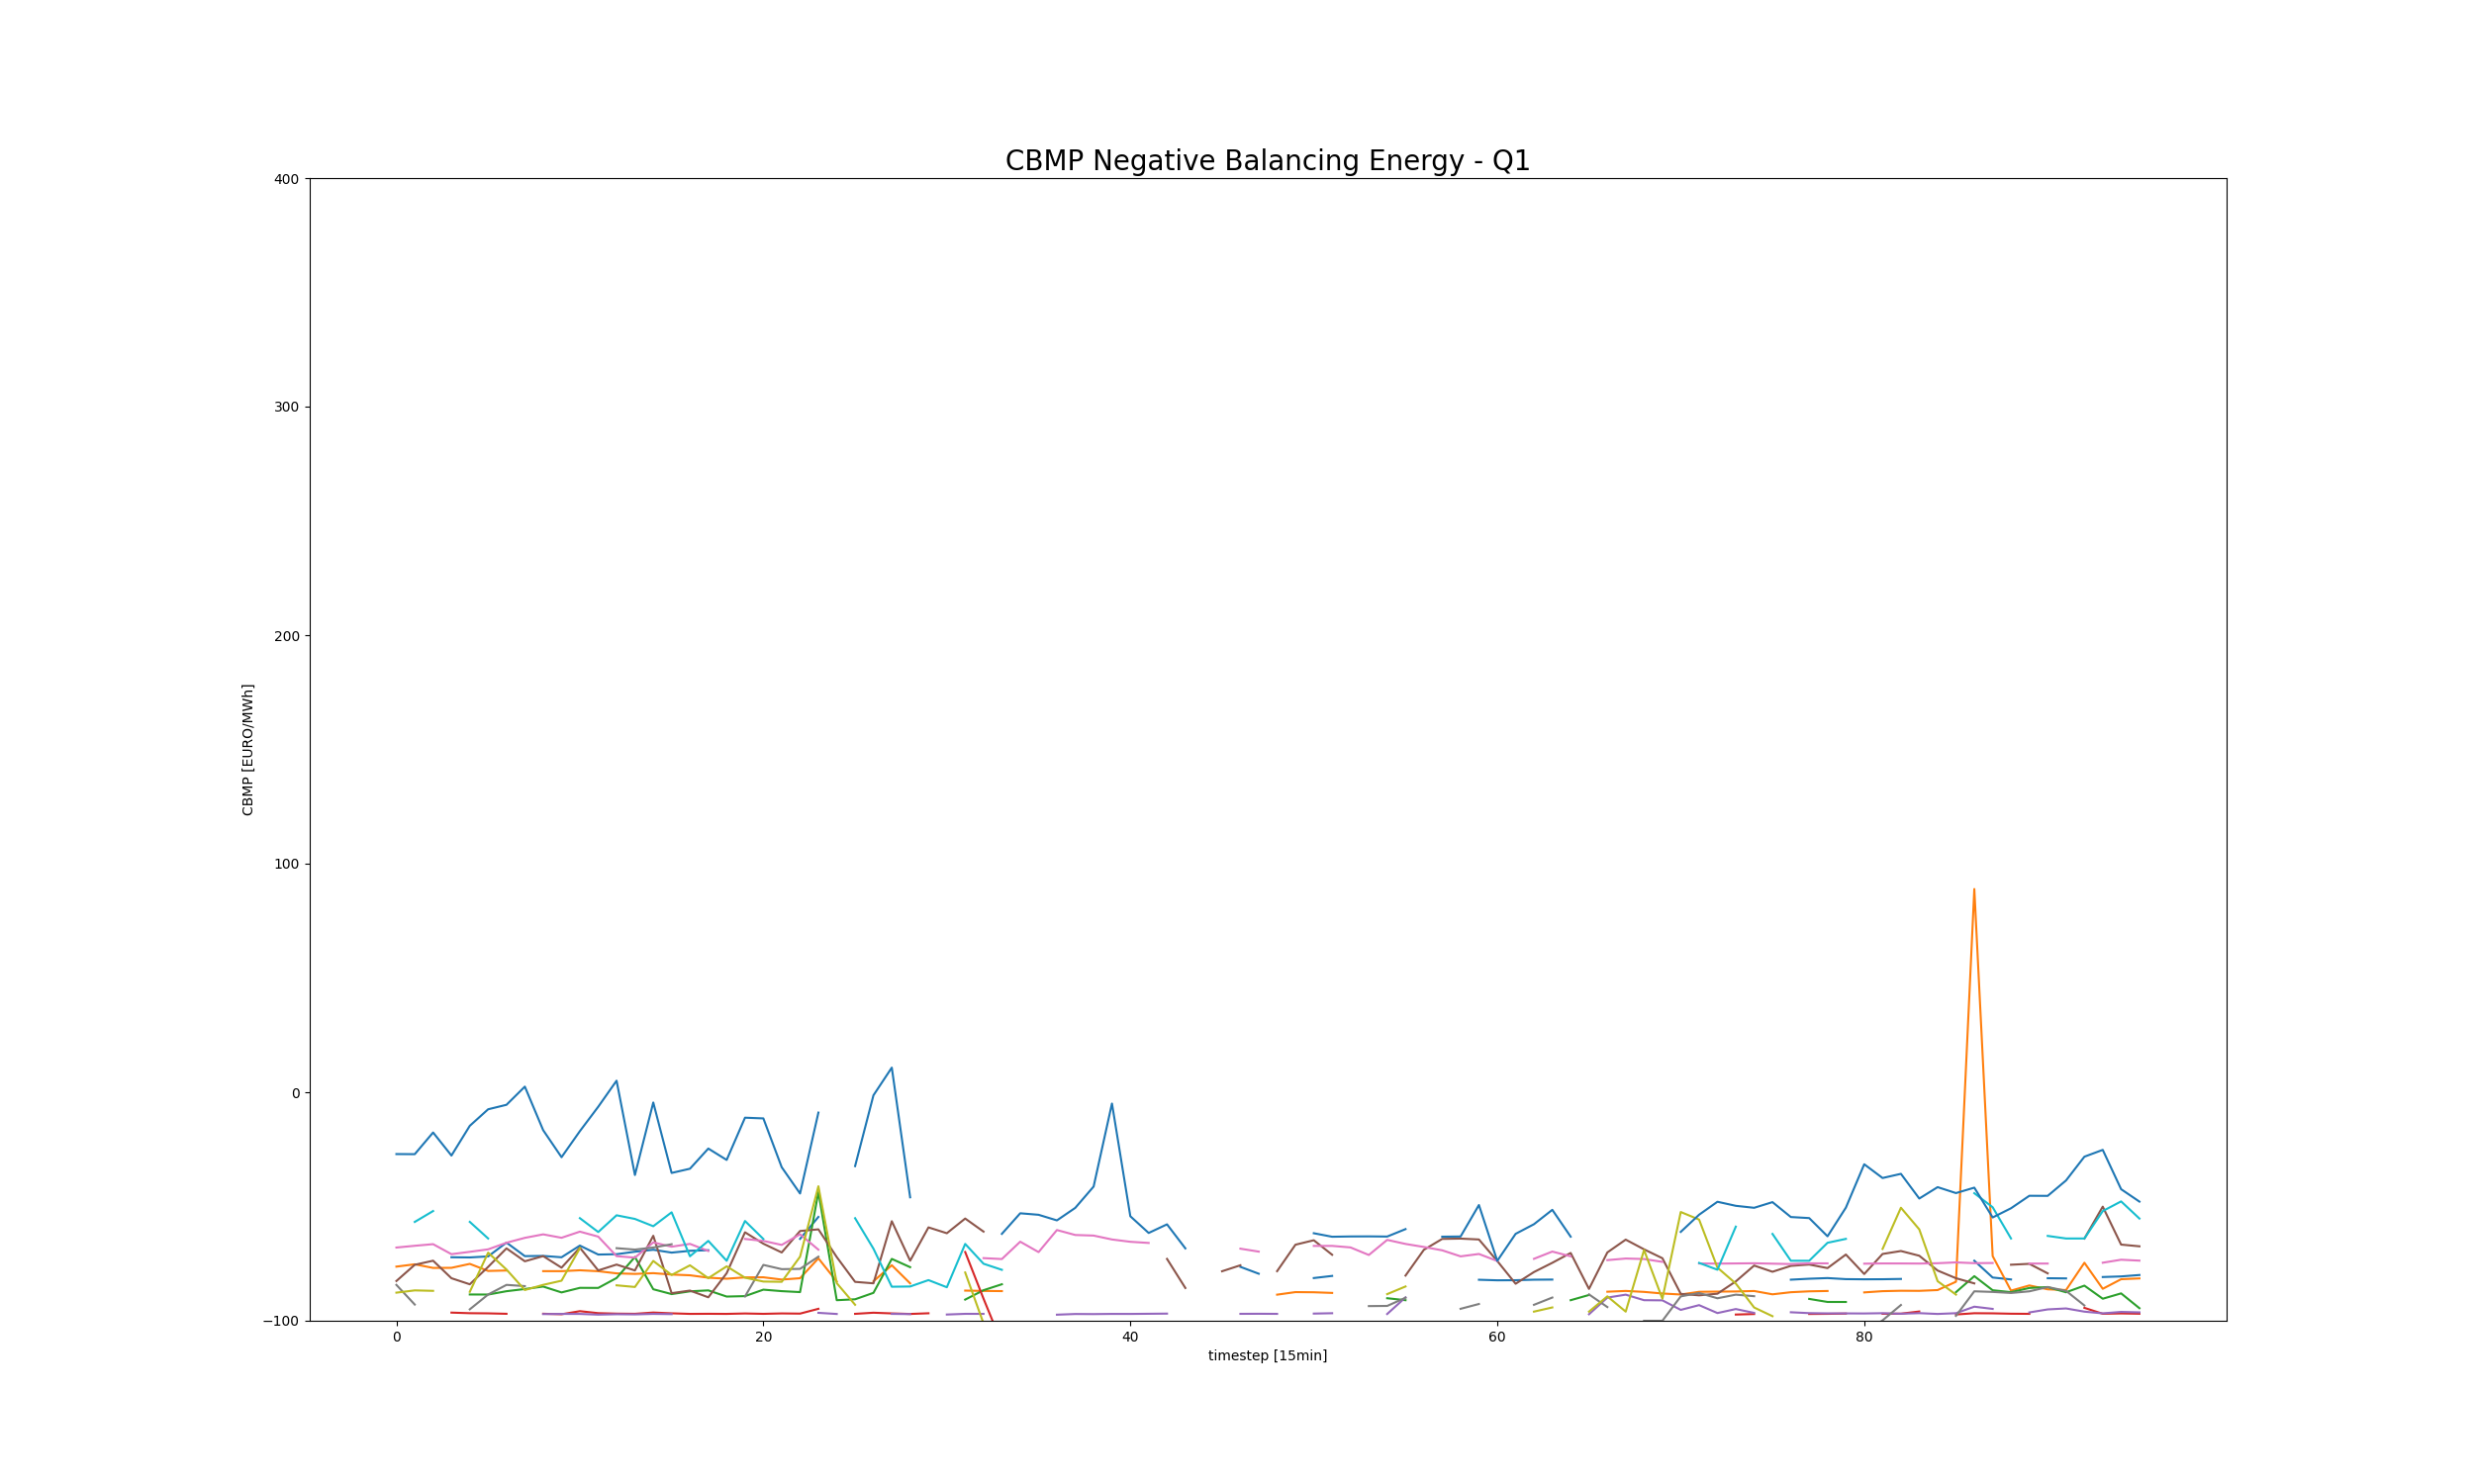
\includegraphics[width=1\linewidth]{pictures/results/CBMP_negBal_Q1.png}
	\caption{CBMP Negative Energy Q1}
	\label{fig:CBMP_negBal_Q1}
\end{figure}


\begin{figure}[H]
	\centering
	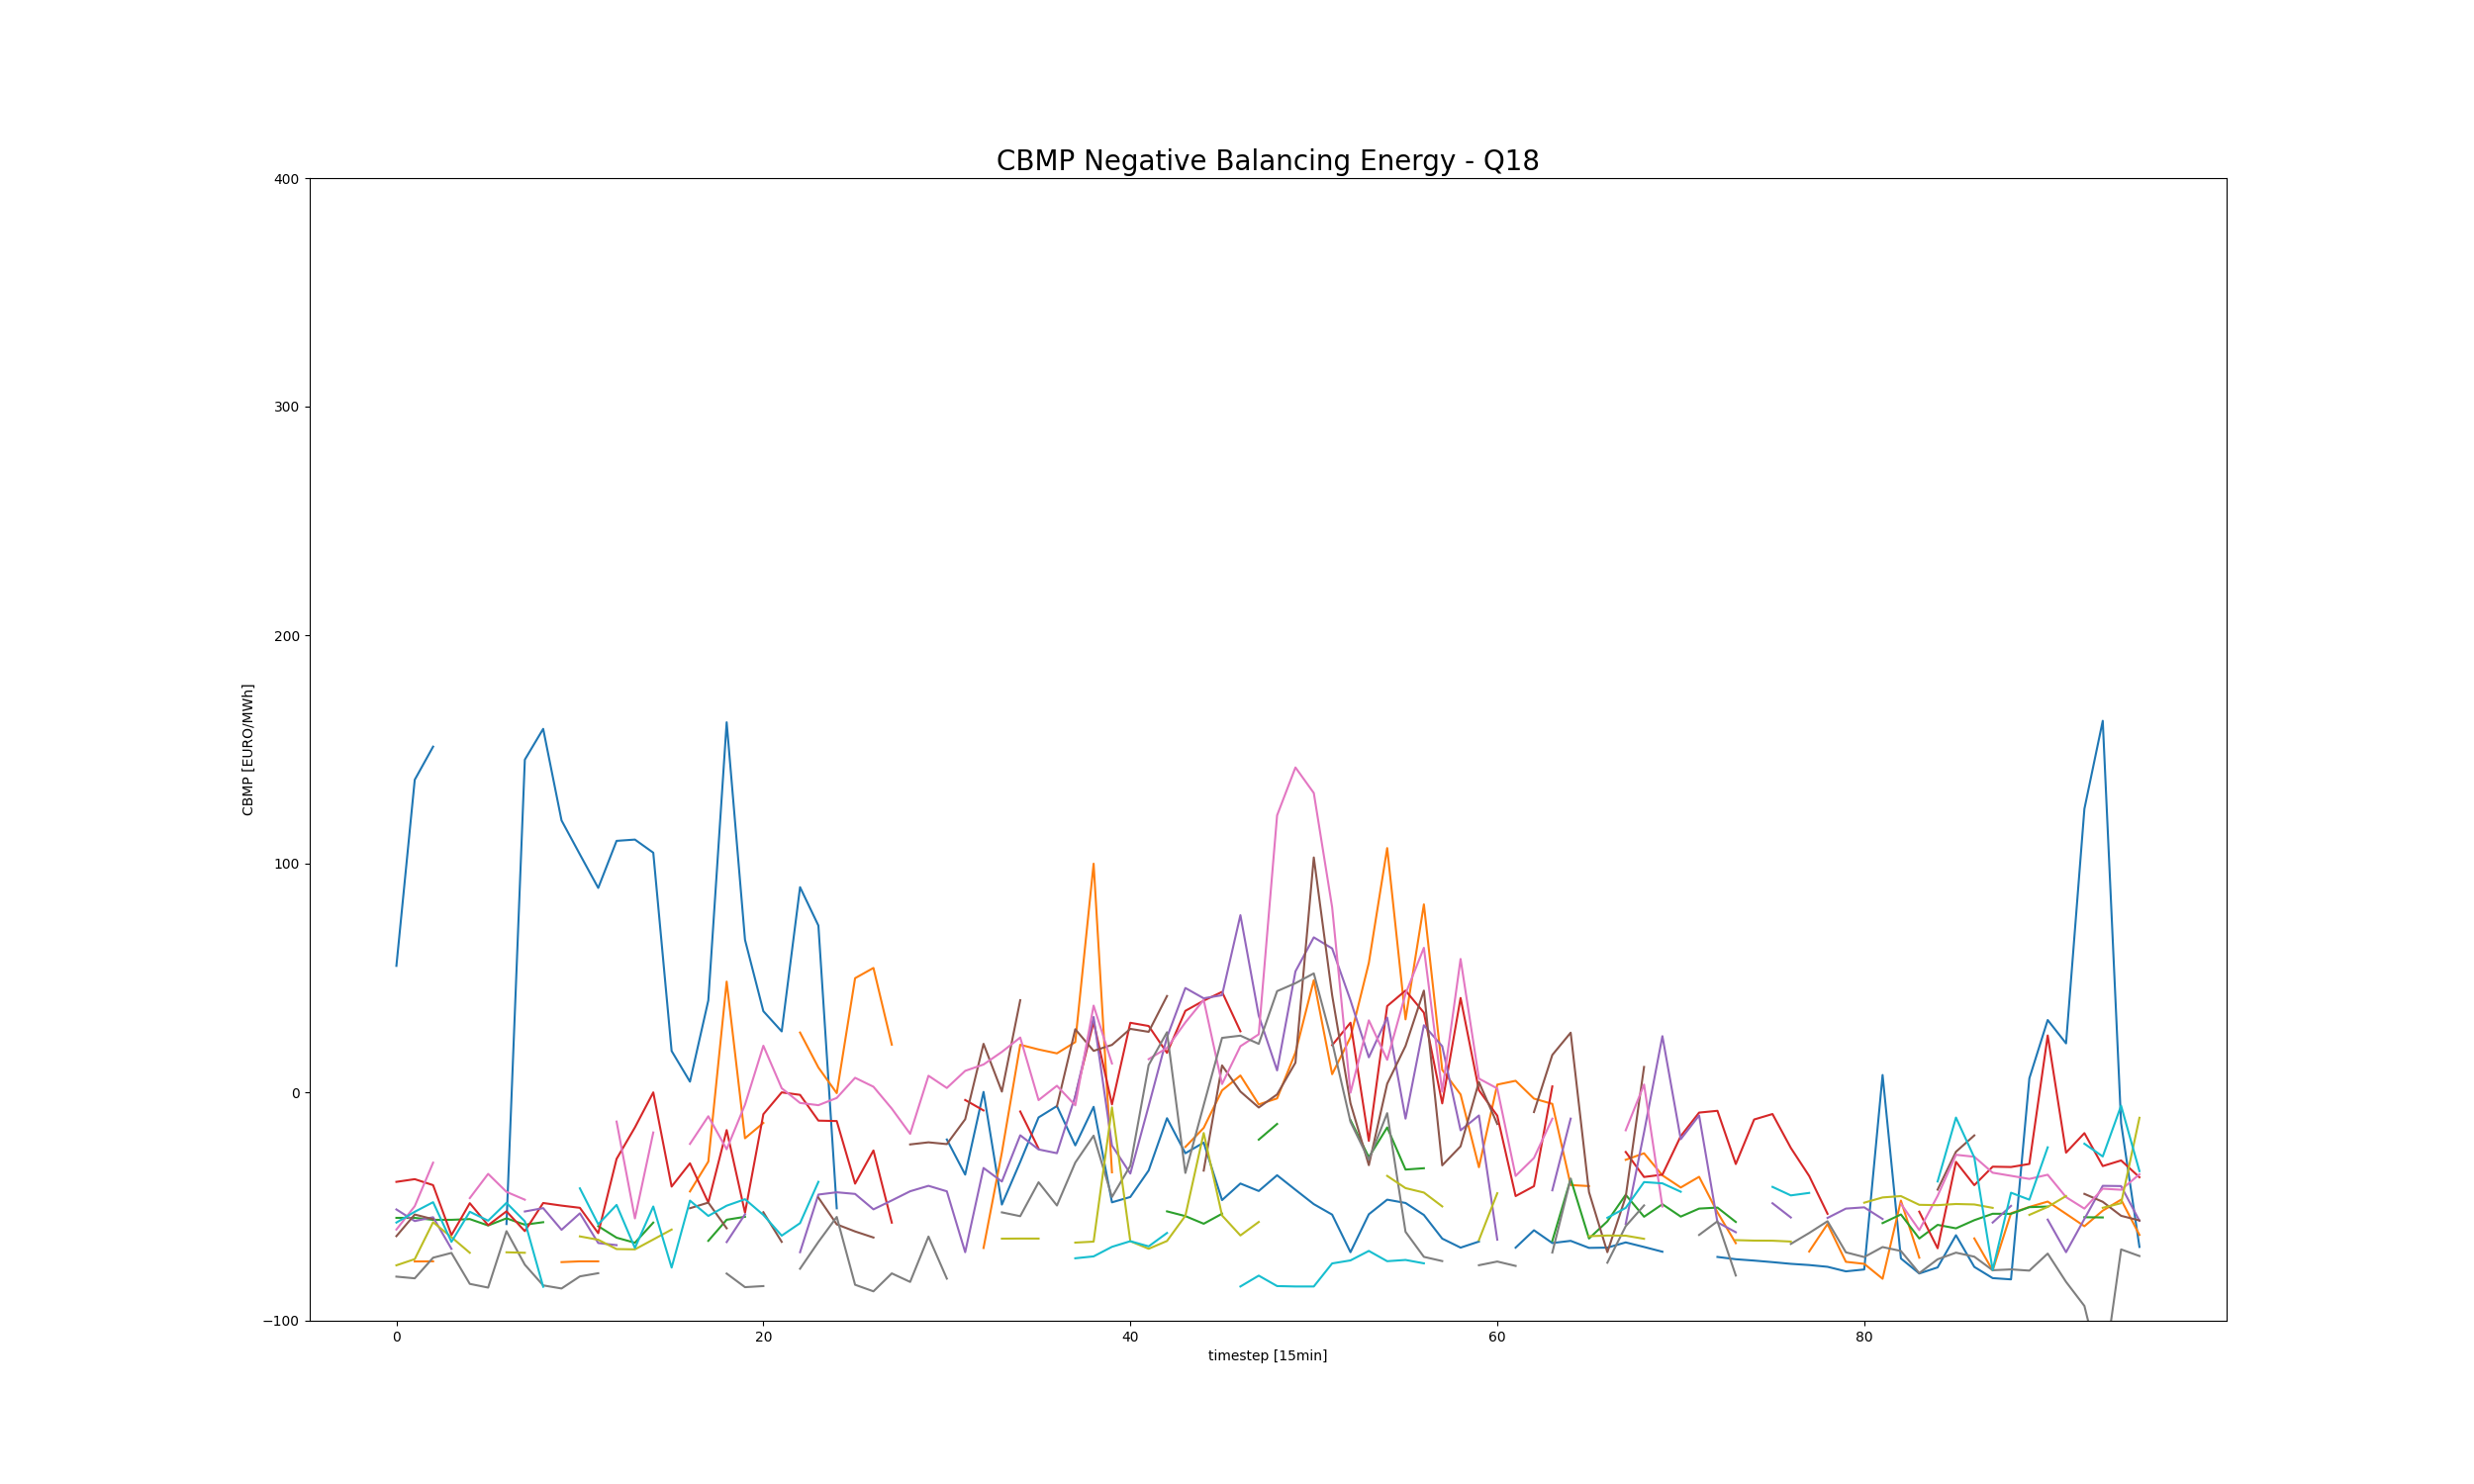
\includegraphics[width=1\linewidth]{pictures/results/CBMP_negBal_Q18.png}
	\caption{CBMP Negative Energy Q18}
	\label{fig:CBMP_negBal_Q18}
\end{figure}


\begin{figure}[H]
	\centering
	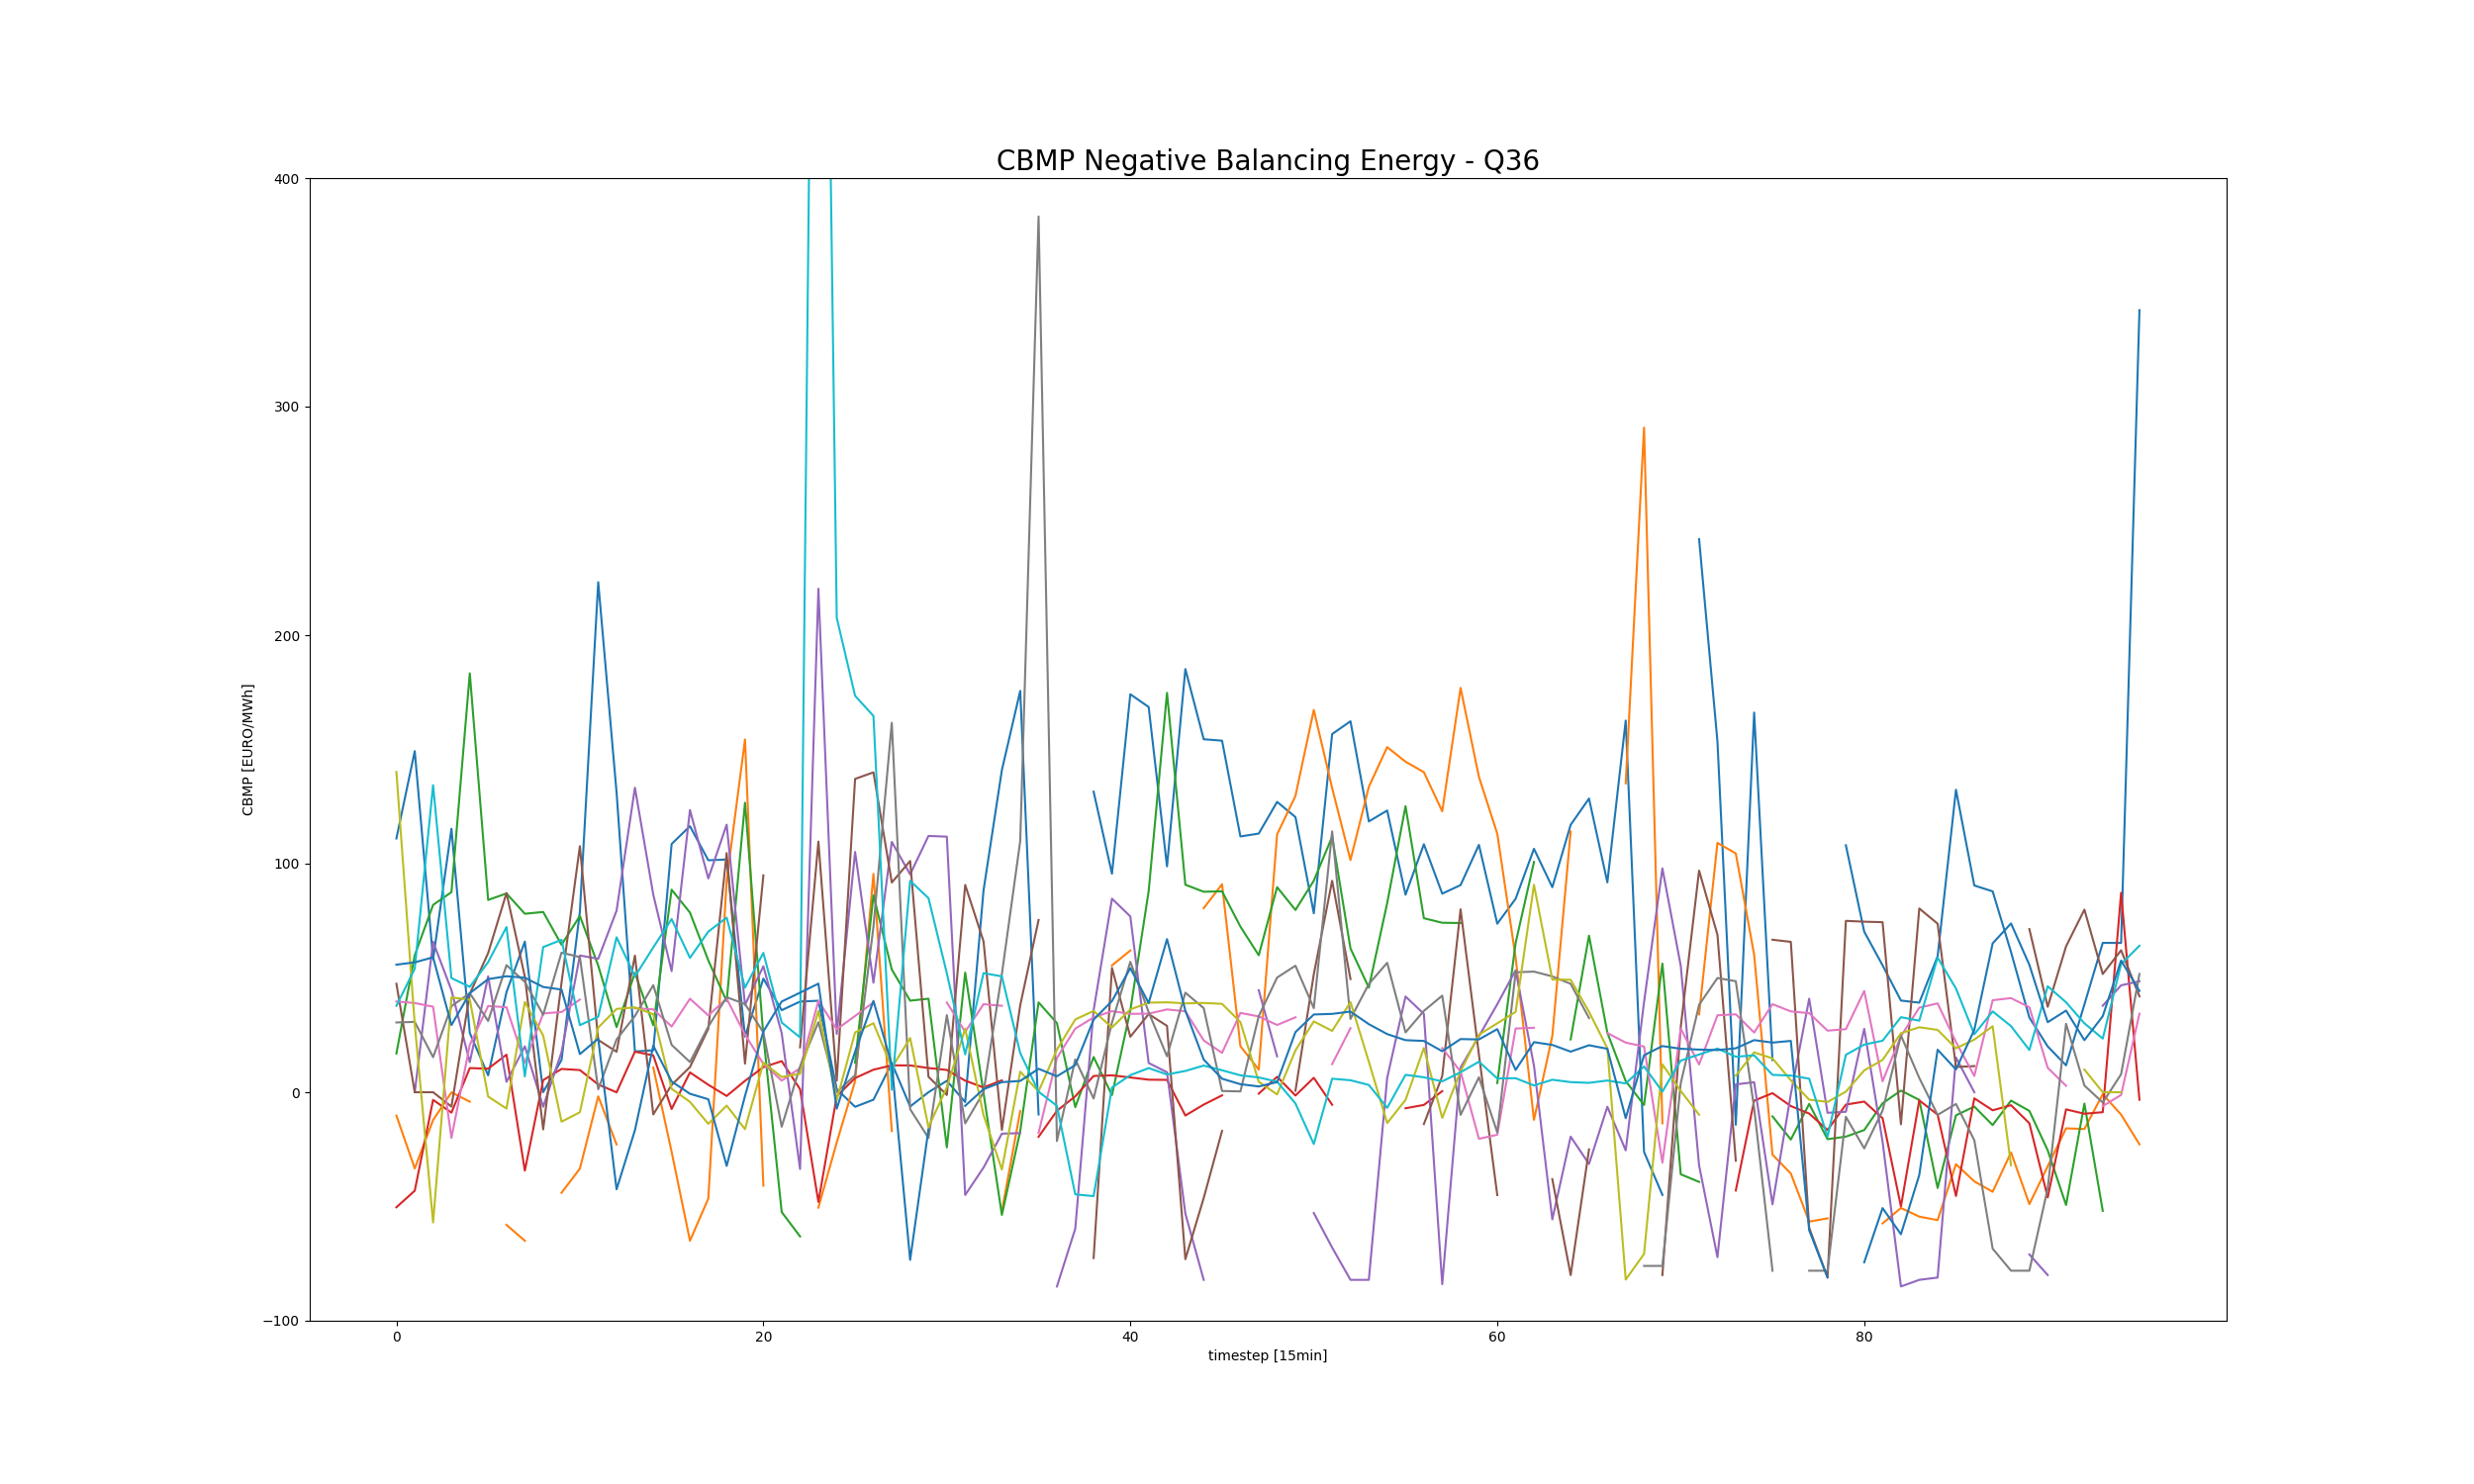
\includegraphics[width=1\linewidth]{pictures/results/CBMP_negBal_Q36.png}
	\caption{CBMP Negative Energy Q36}
	\label{fig:CBMP_negBal_Q36}
\end{figure}

\begin{figure}
	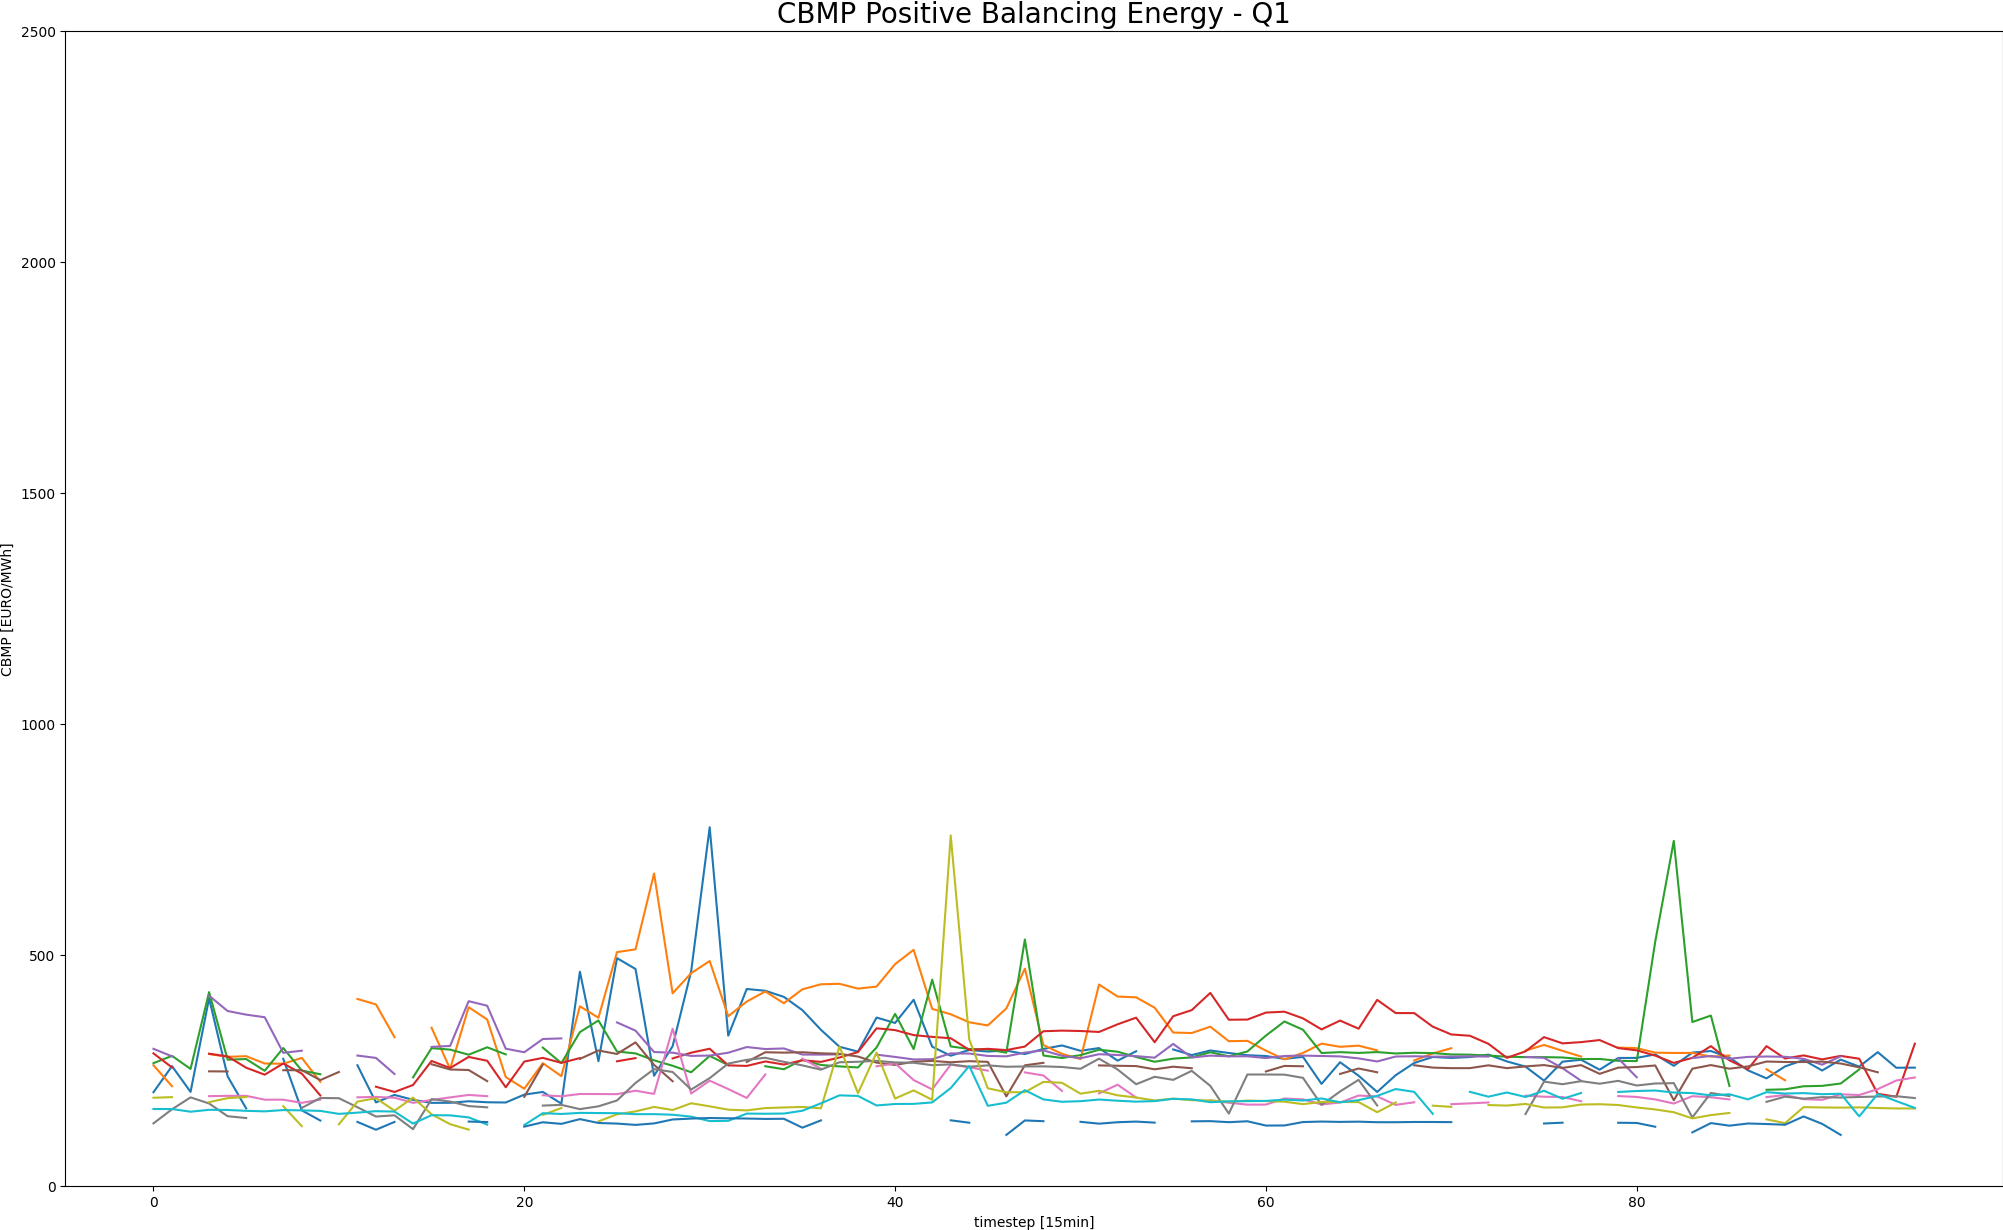
\includegraphics[width=1\linewidth]{pictures/results/CBMP_PosBal_Q1.png}
	\caption{CBMP Positive Energy Q1}
	\label{fig:CBMP_PosBal_Q1}
\end{figure}

\begin{figure}
	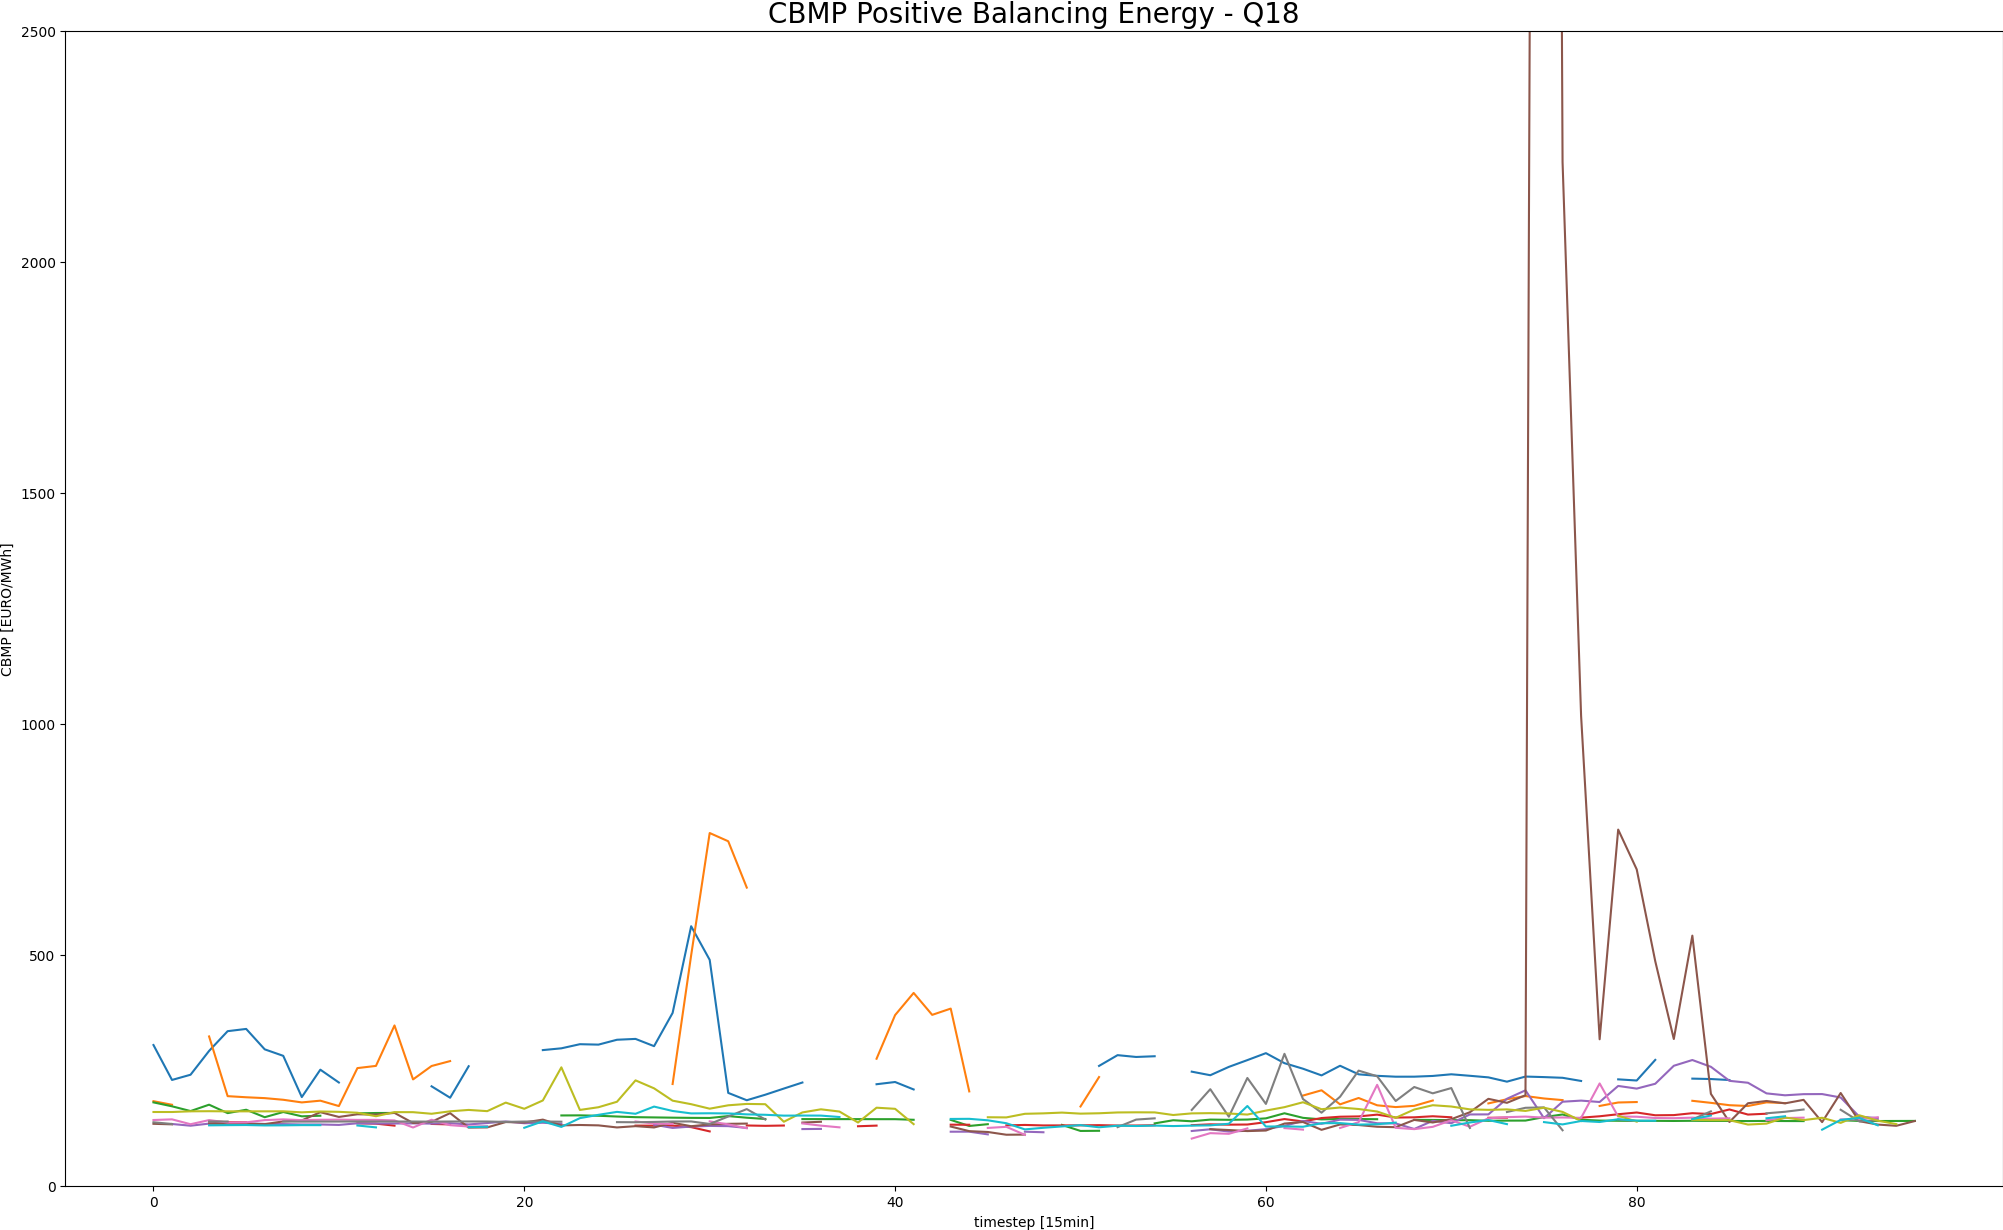
\includegraphics[width=1\linewidth]{pictures/results/CBMP_PosBal_Q18.png}
	\caption{CBMP Positive Energy Q18}
	\label{fig:CBMP_PosBal_Q18}
\end{figure}
\begin{figure}
	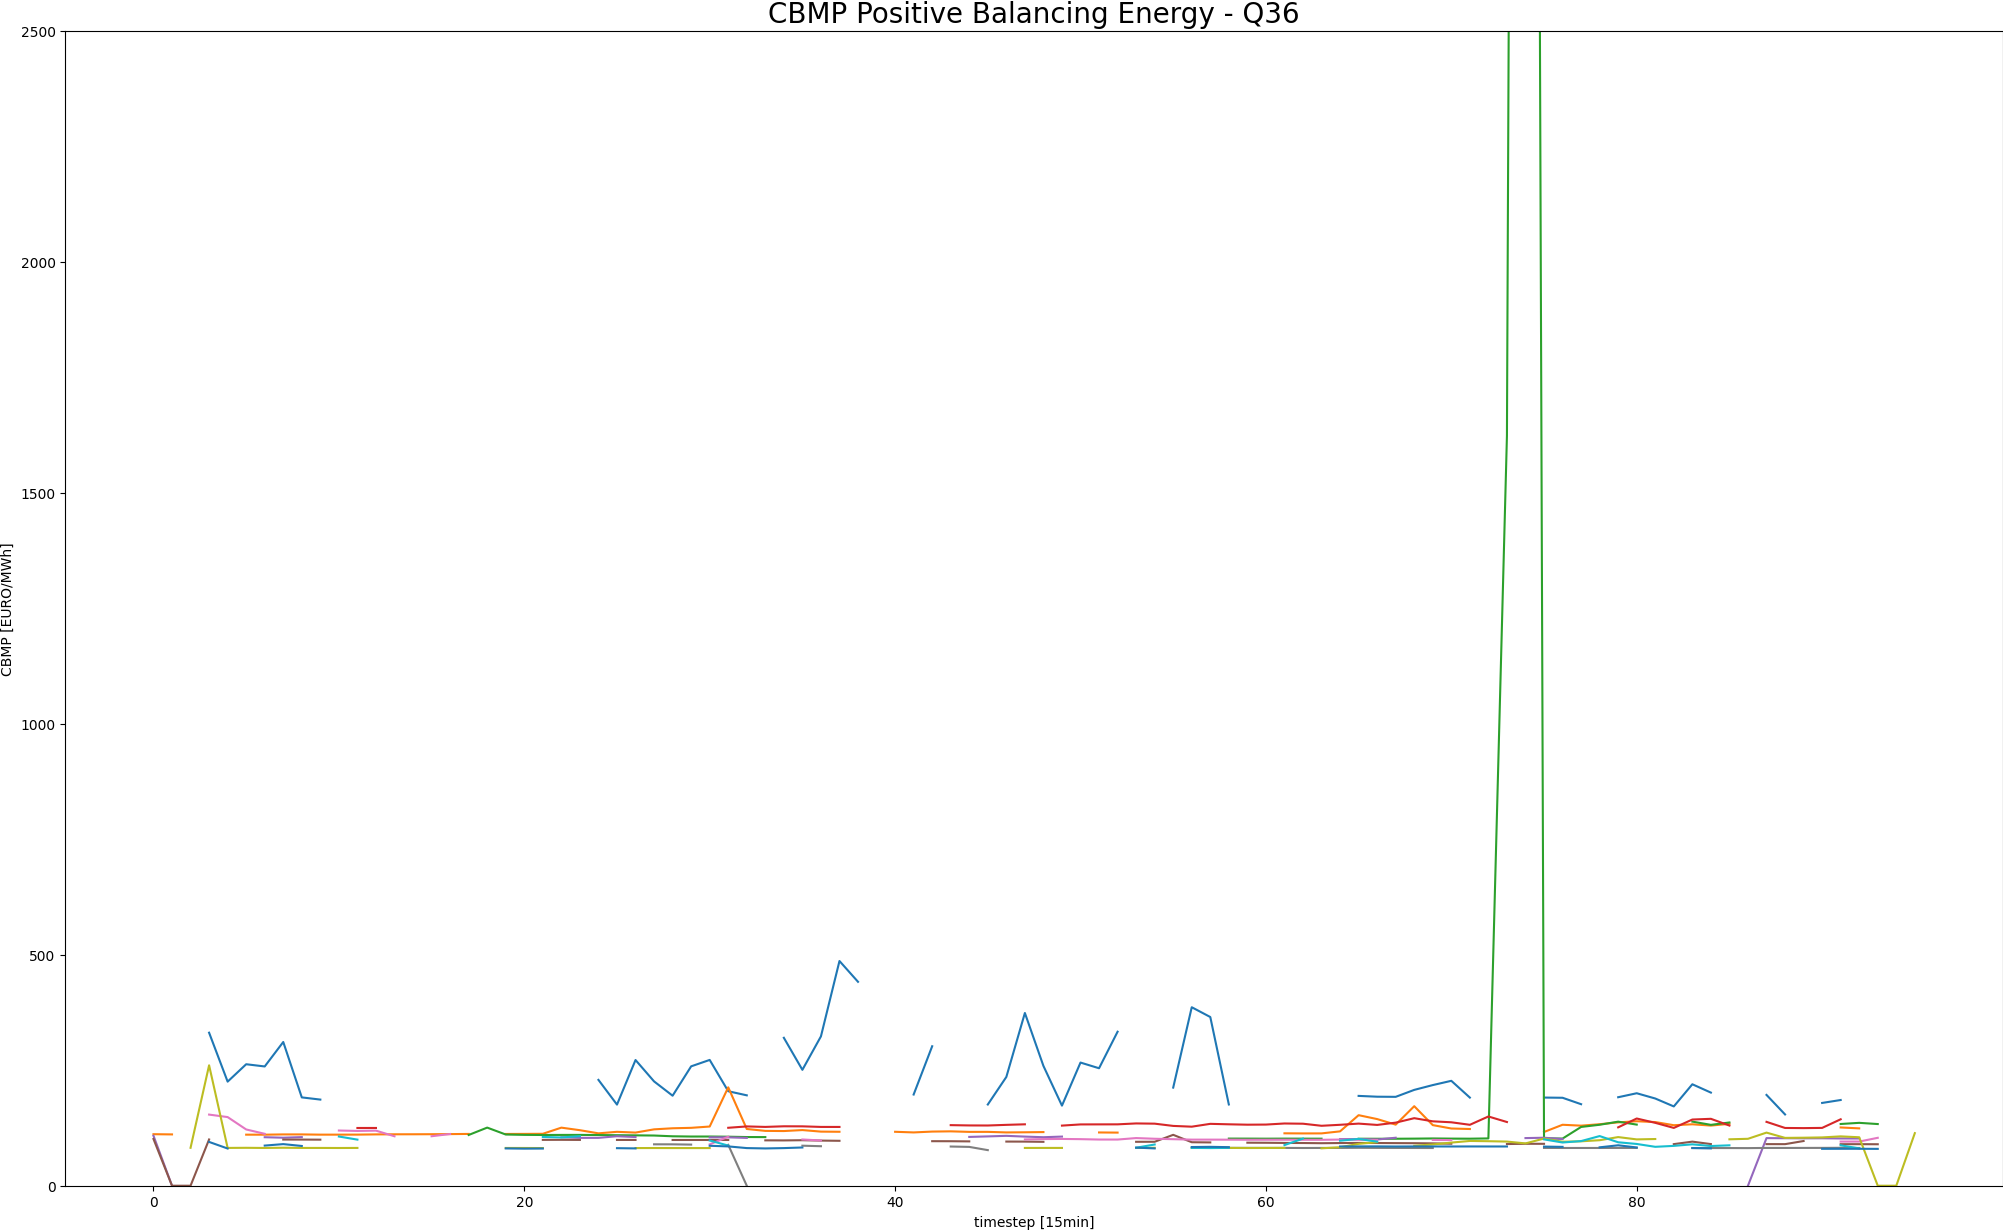
\includegraphics[width=1\linewidth]{pictures/results/CBMP_PosBal_Q36.png}
	\caption{CBMP Positive Energy Q36}
	\label{fig:CBMP_PosBal_Q36}
\end{figure}

Für den selben Zeitabschnitt lässt sich der DA Markt wie folgt zusammenfassen:
\begin{figure}[H]
	\centering
	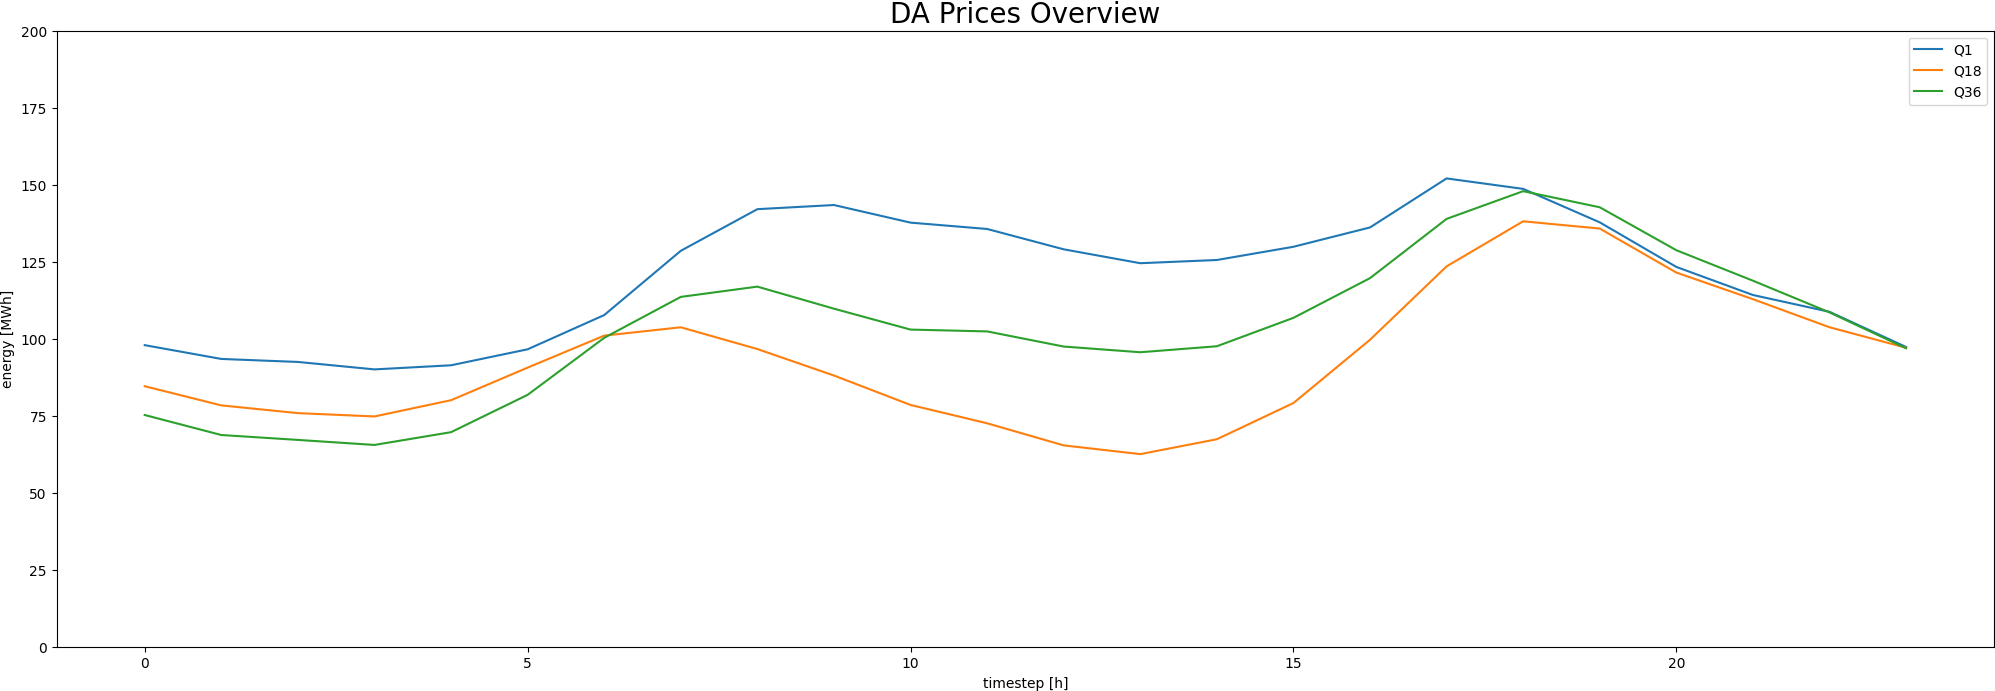
\includegraphics[width=1\linewidth]{pictures/results/DAPrices.png}
	\caption{DA Prices}
	\label{fig:DAPrices}
\end{figure}
\begin{figure}
	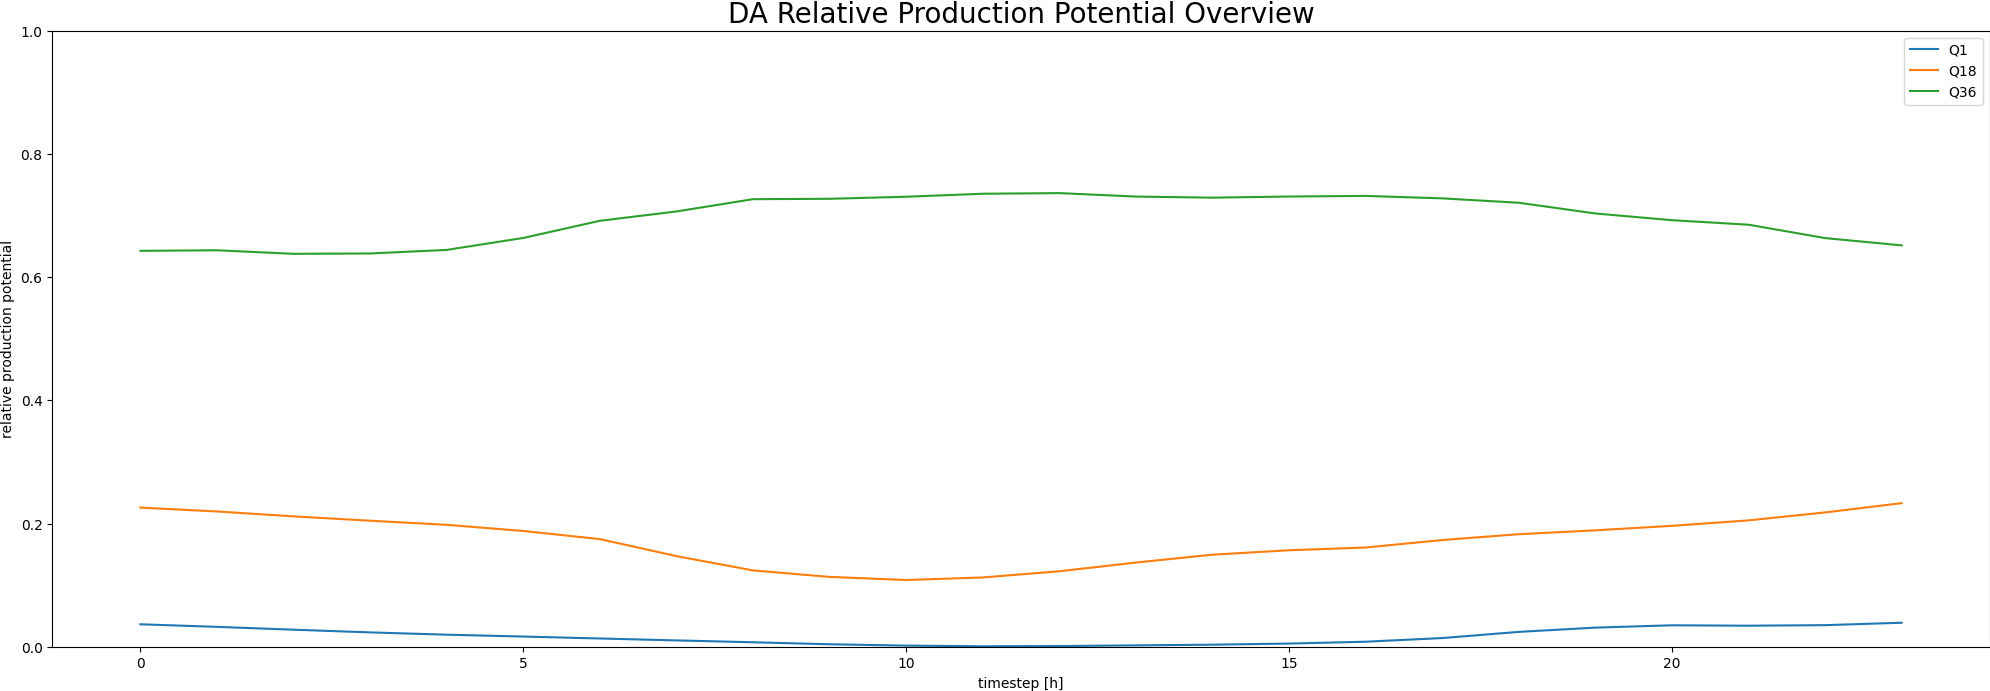
\includegraphics[width=1\linewidth]{pictures/results/DAProd.png}
	\caption{DA Production}
	\label{fig:DAProd}
\end{figure}

Außerdem stellt sich der entsprechende RL Markt wie folgt dar:

\begin{figure}[H]
	\centering
	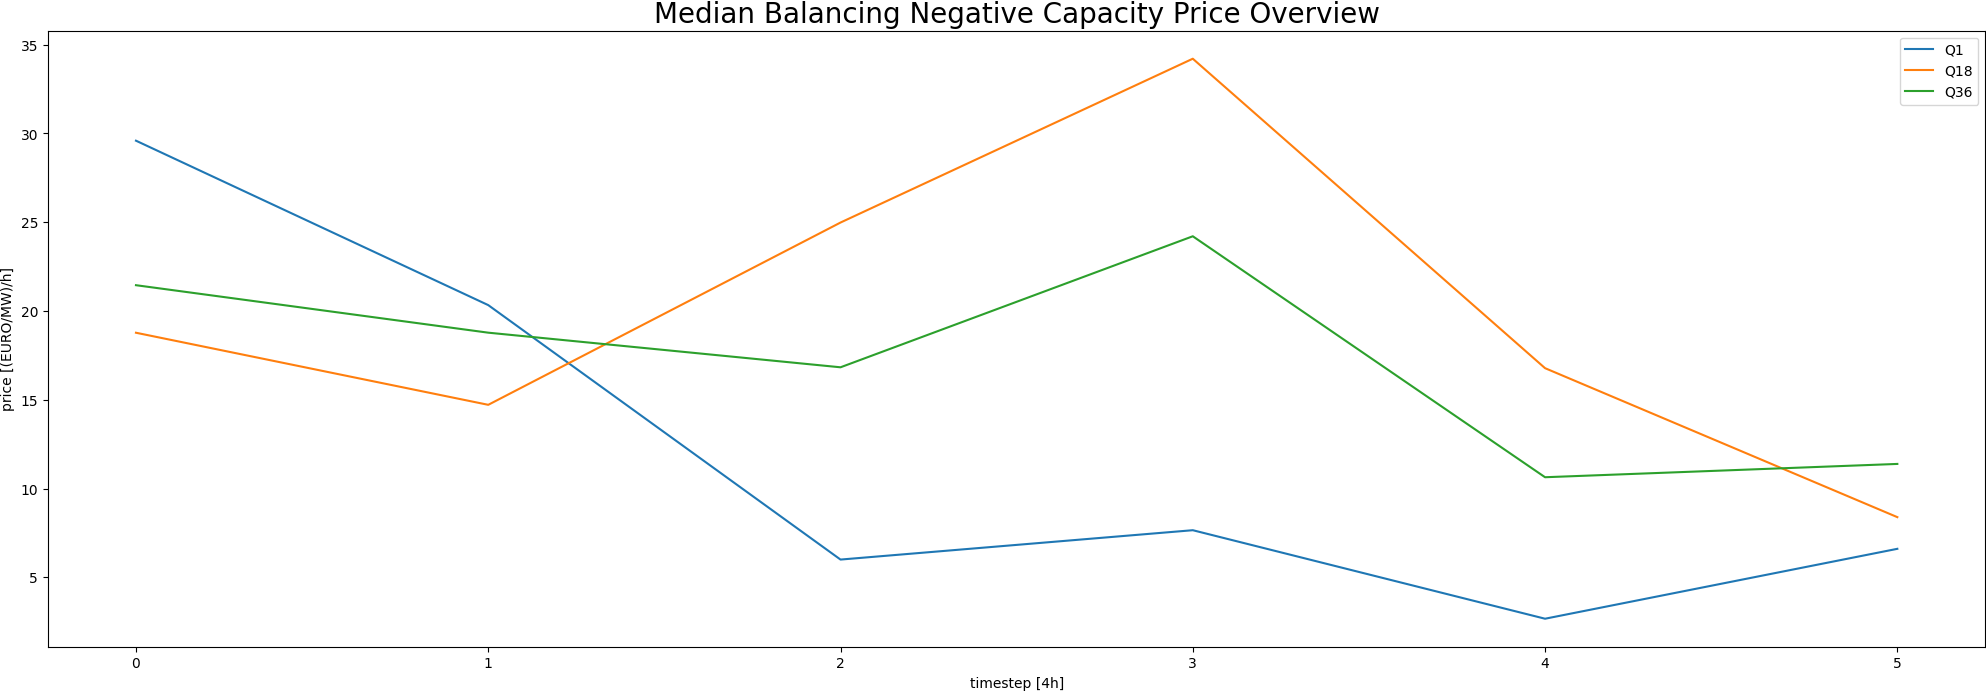
\includegraphics[width=1\linewidth]{pictures/results/RL_negPrice_Overview.png}
	\caption{RL Negative Prices}
	\label{fig:RL_negPrice_Overview}
\end{figure}
\begin{figure}
	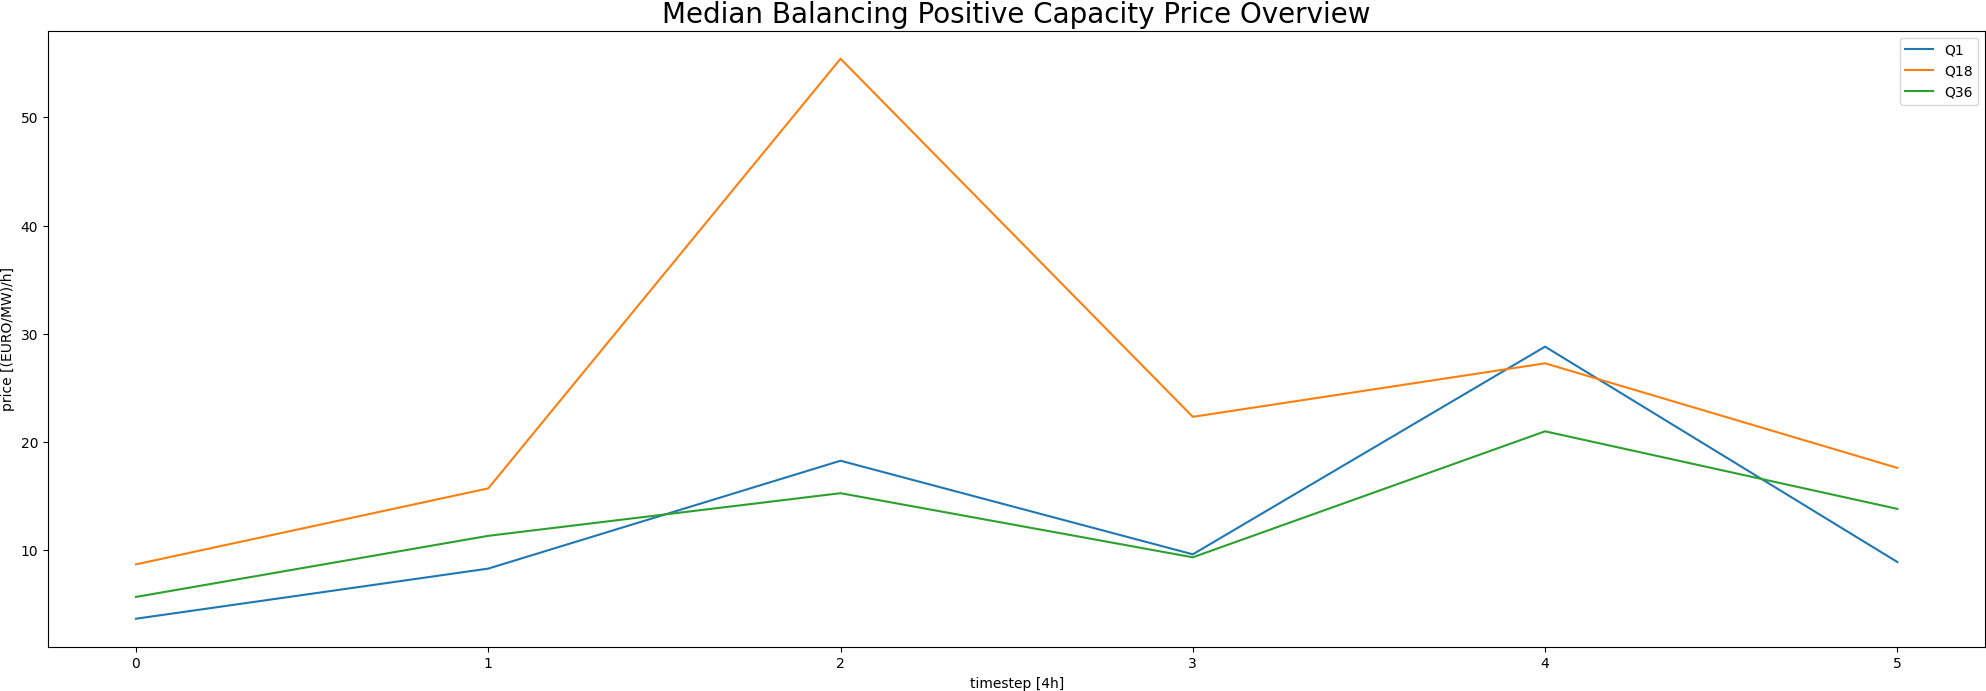
\includegraphics[width=1\linewidth]{pictures/results/RL_posPrice_Overview.png}
	\caption{RL Negative Prices}
	\label{fig:RL_posPrice_Overview}
\end{figure}

\section{Model Results}

\begin{figure}[H]
	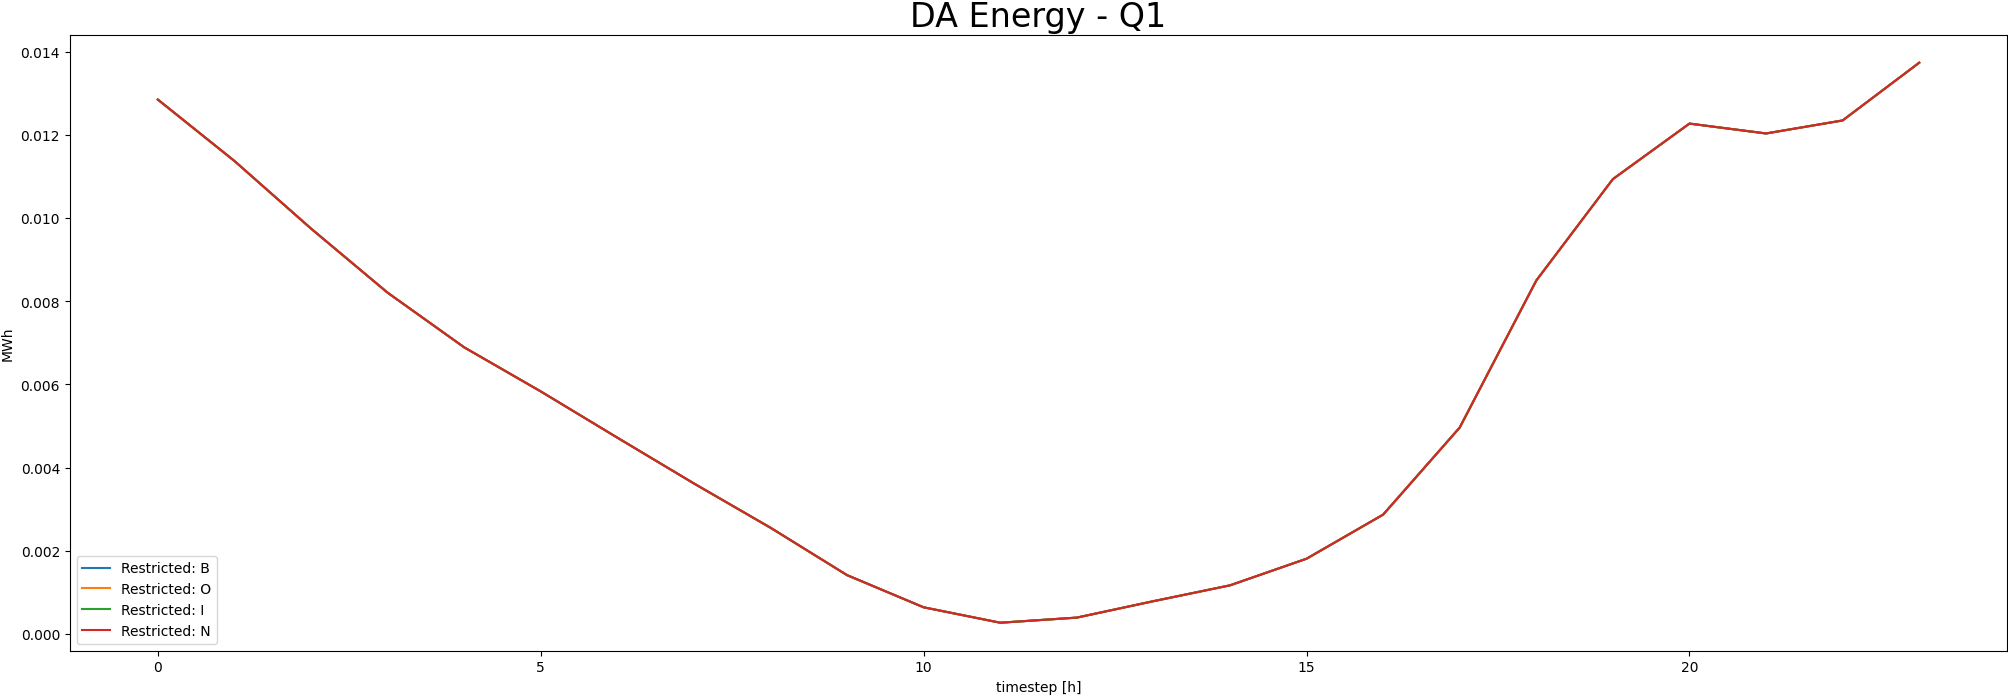
\includegraphics[width=1\linewidth]{pictures/results/DA Energy - Q1.png}
	\caption{DA Energy - Q1}
	\label{fig:DA Energy - Q1}
\end{figure}

\begin{figure}[H]
	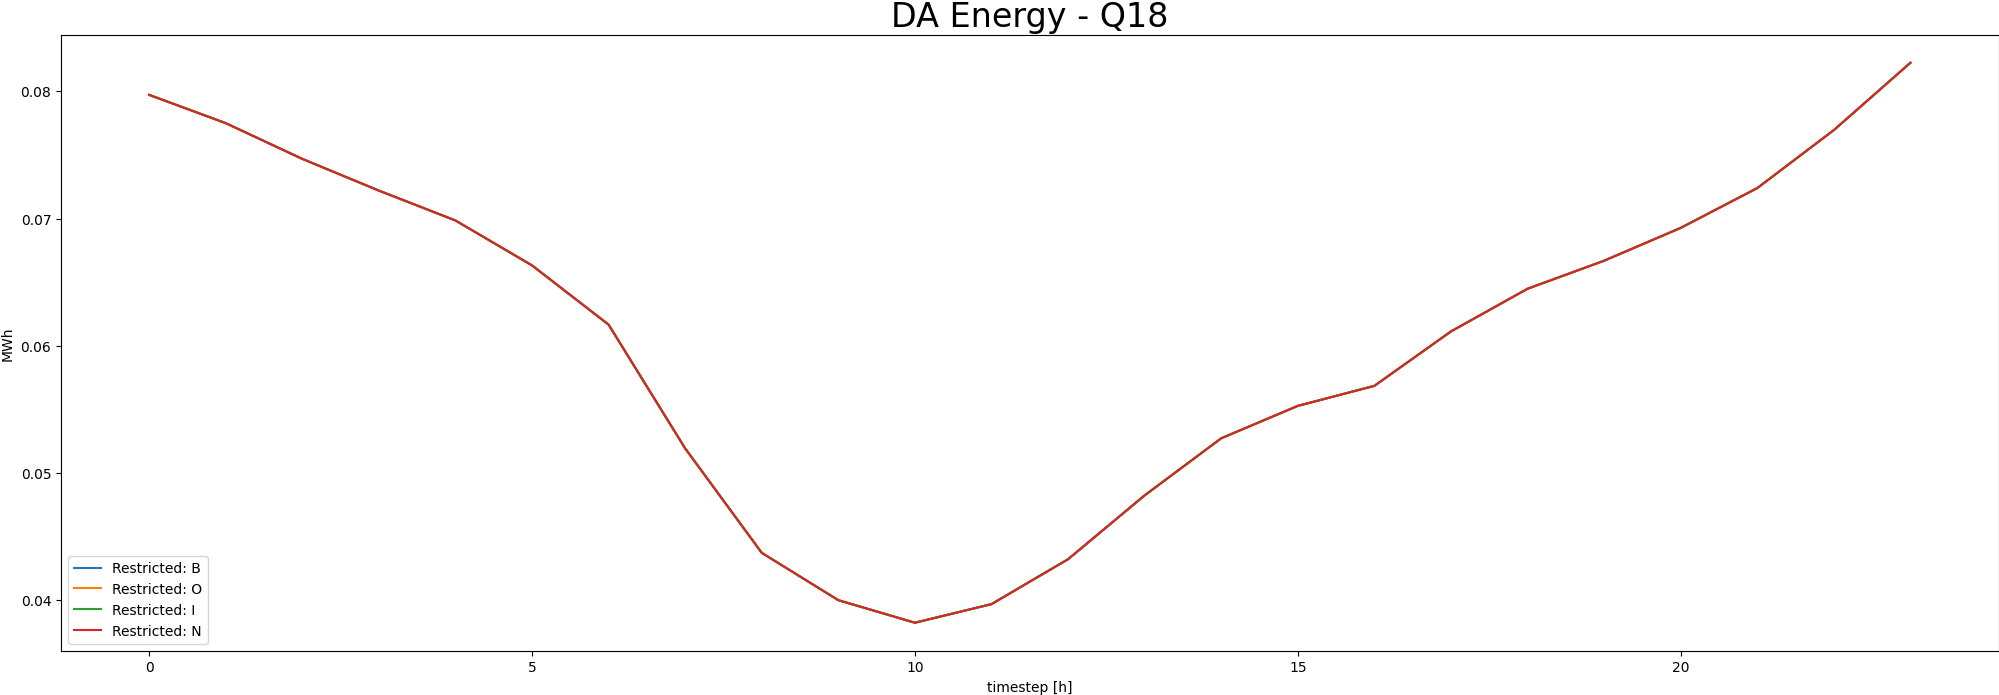
\includegraphics[width=1\linewidth]{pictures/results/DA Energy - Q18.png}
	\caption{DA Energy - Q18}
	\label{fig:DA Energy - Q18}
\end{figure}

\begin{figure}[H]
	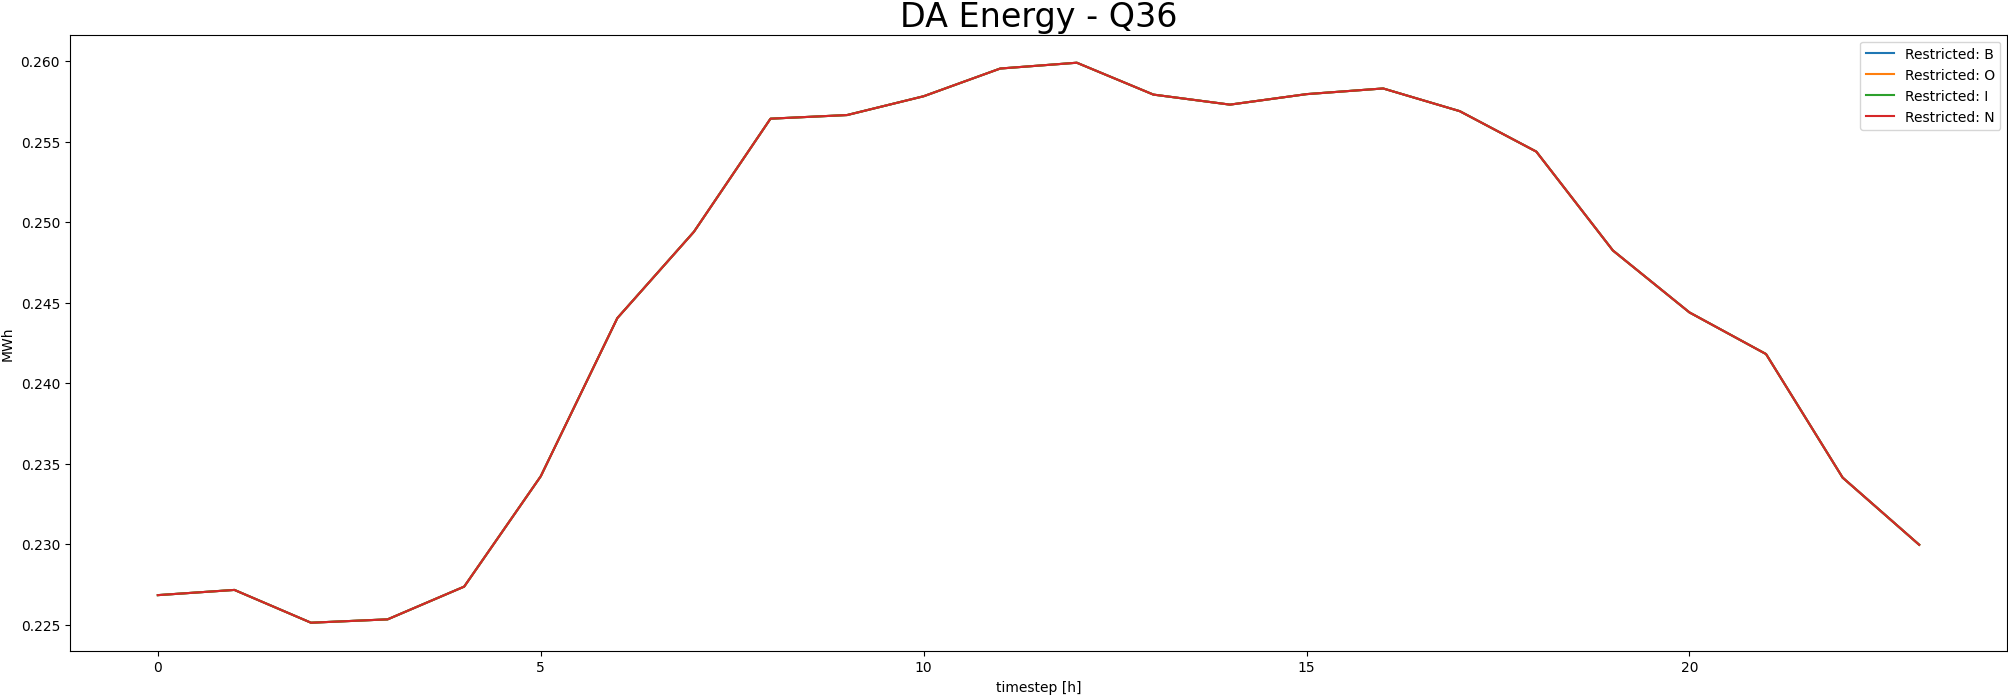
\includegraphics[width=1\linewidth]{pictures/results/DA Energy - Q36.png}
	\caption{DA Energy - Q36}
	\label{fig:DA Energy - Q36}
\end{figure}
\begin{figure}[H]
	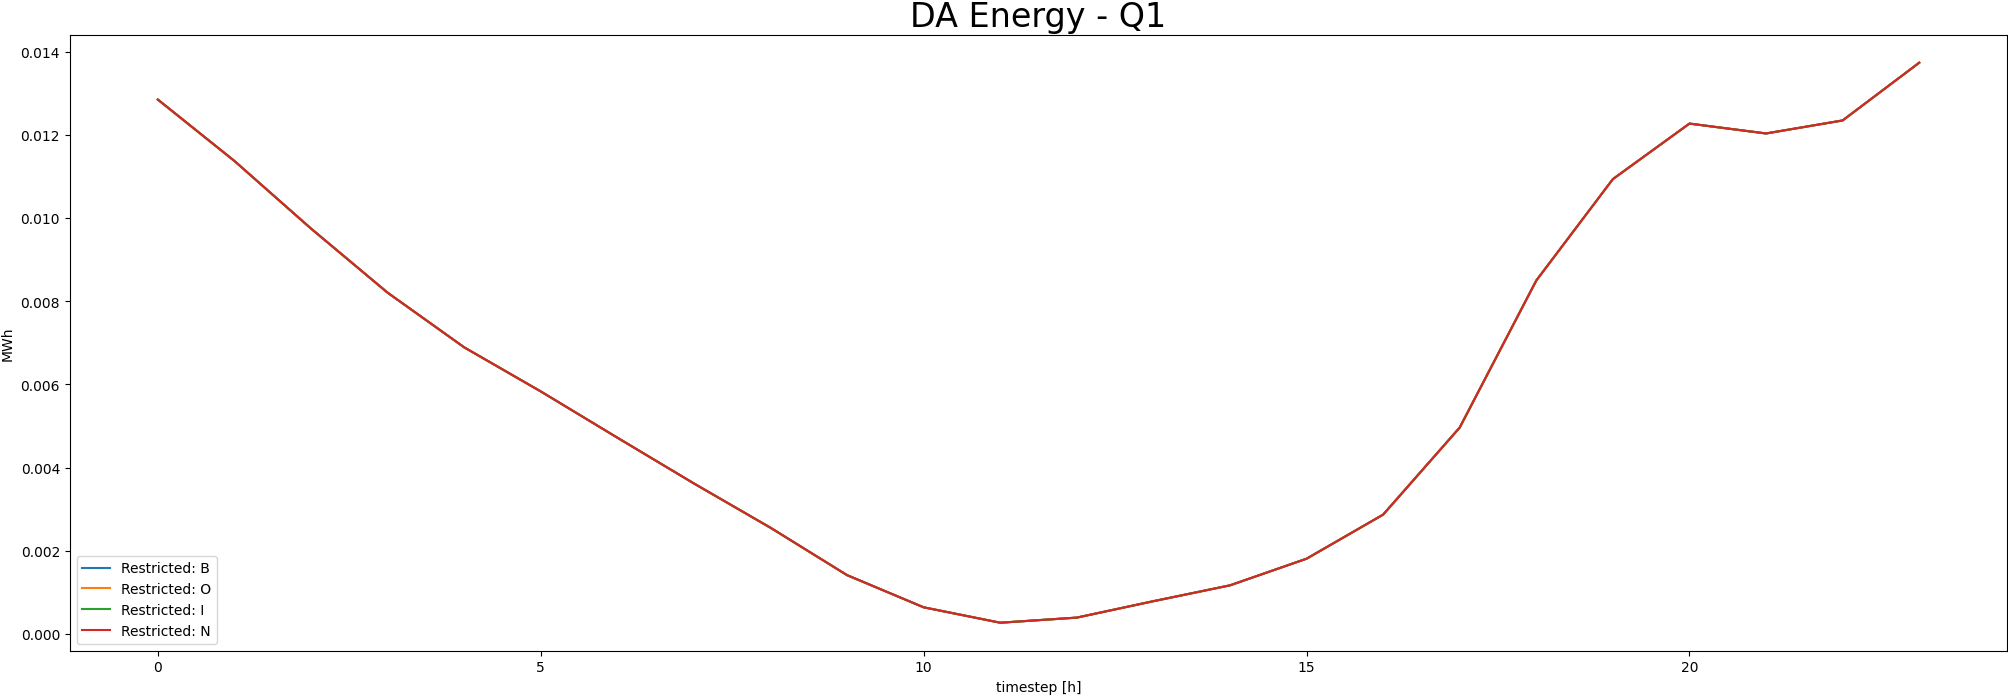
\includegraphics[width=1\linewidth]{pictures/results/DA Energy - Q1.png}
	\caption{Balance Capacity - Q1}
	\label{fig:Balance Capacity - Q1}
\end{figure}

\begin{figure}[H]
	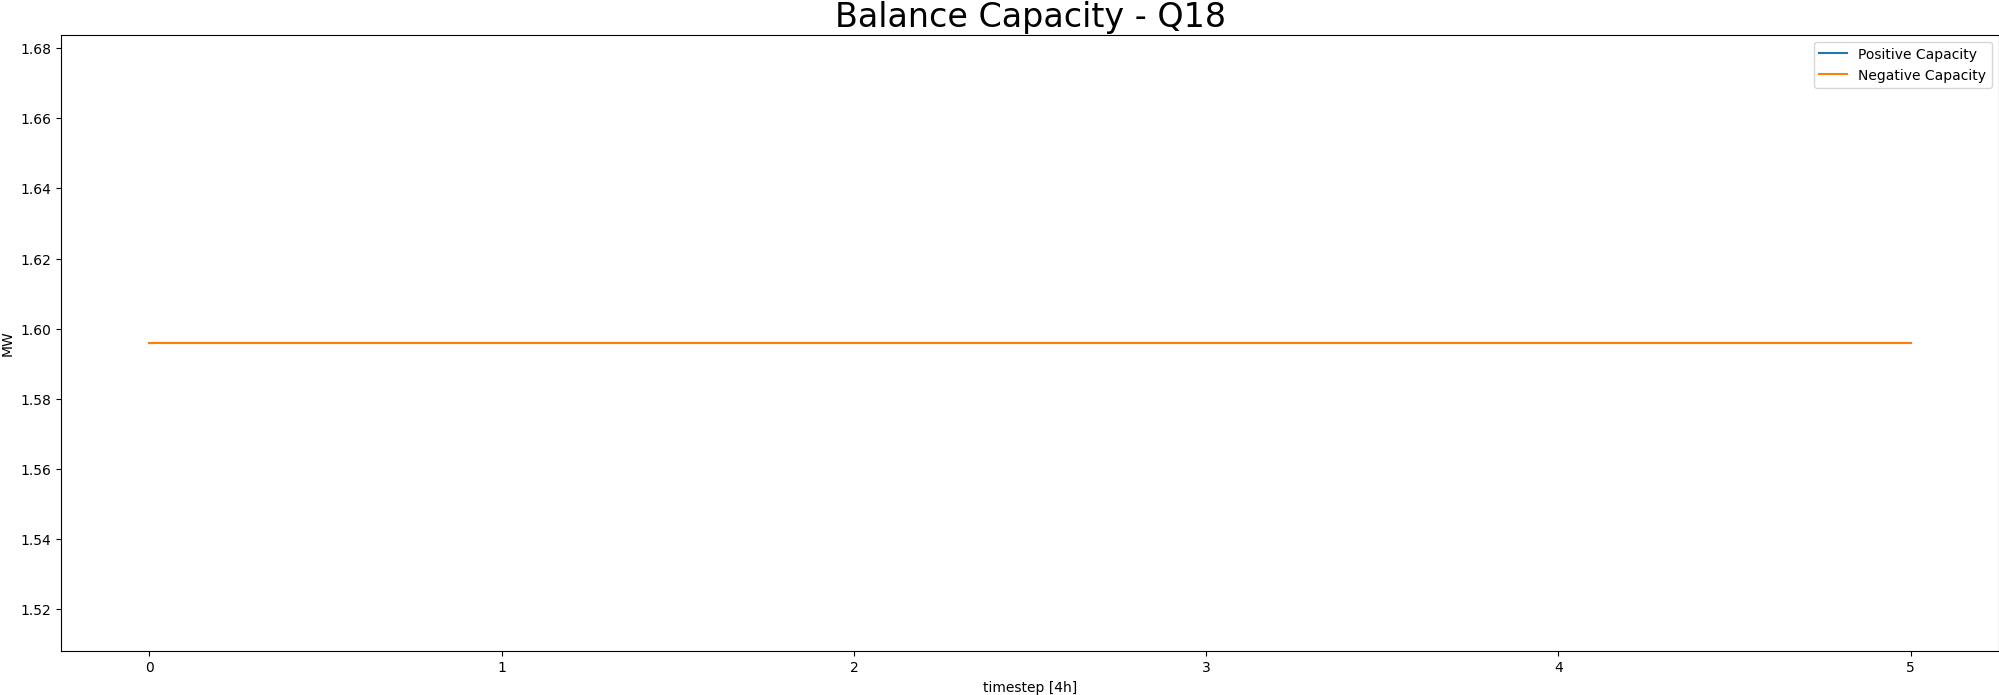
\includegraphics[width=1\linewidth]{pictures/results/Balance Capacity - Q18.png}
	\caption{Balance Capacity - Q18}
	\label{fig:Balance Capacity - Q18}
\end{figure}

\begin{figure}[H]
	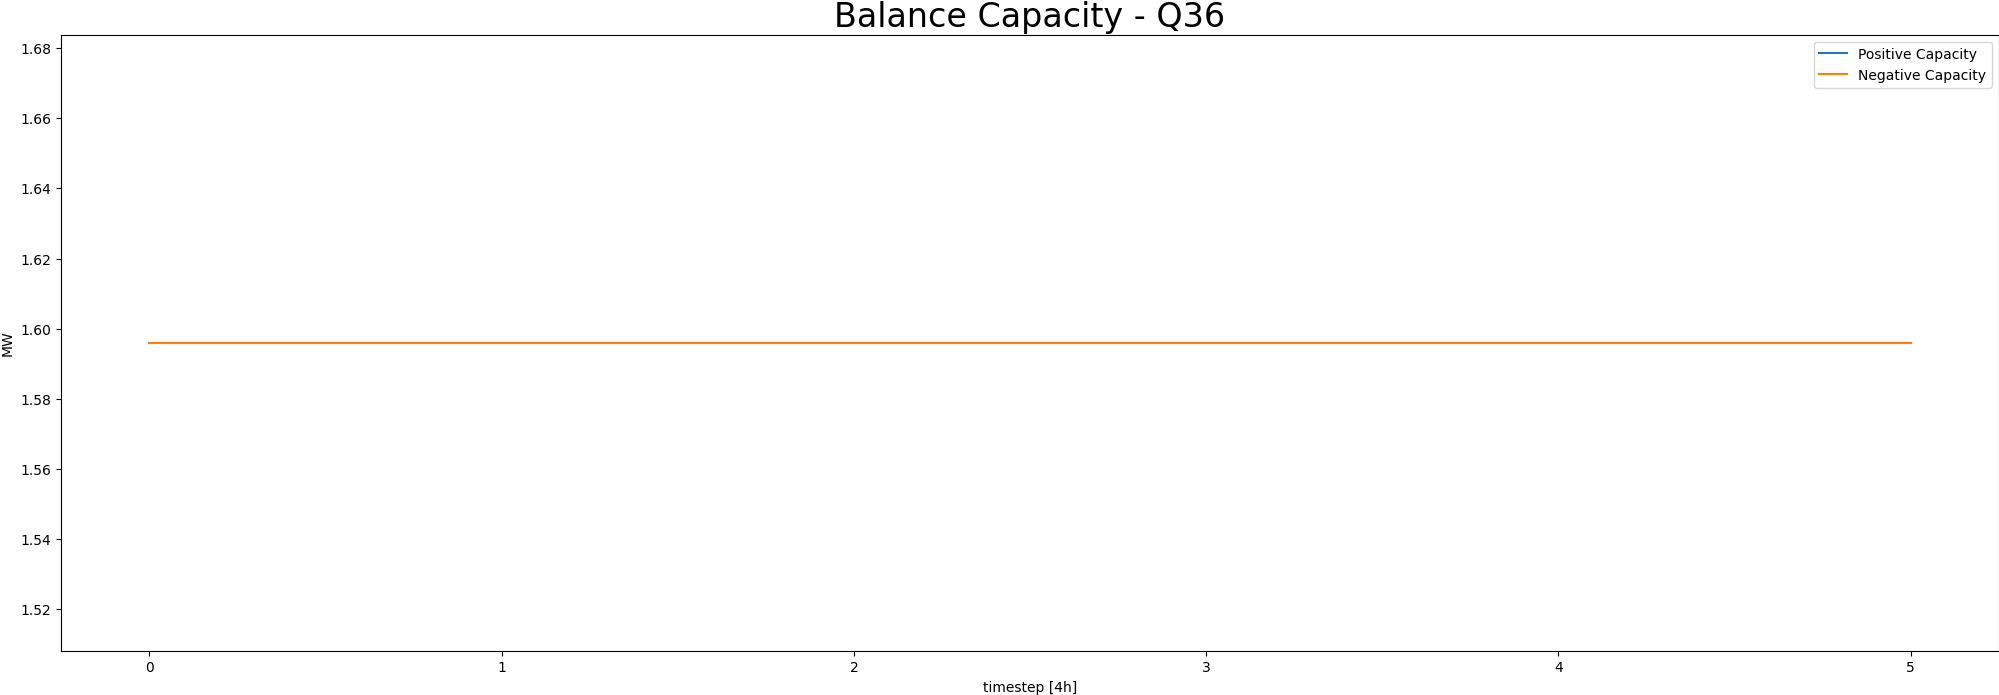
\includegraphics[width=1\linewidth]{pictures/results/Balance Capacity - Q36.png}
	\caption{Balance Capacity - Q36}
	\label{fig:Balance Capacity - Q36}
\end{figure}







\section{Digital Appendix}



%% *** local page settings ***
\addtocontents{toc}{\protect\setcounter{tocdepth}{+1}} %reset the decreased depth of the appendix entry in the ToC
\label{subsec:Bibliography}
\printbibliography[title={Bibliography}]
%% change chapter title to german if necessary



ChatGPT was utilized in this work for the following purposes:
\begin{itemize}
	\item As a search tool for specific functions.
	\item As an aid in refining formulations.
\end{itemize}
All suggestions were carefully reviewed and assessed individually.



\begin{center}
	\textbf{Statement of authorship}
\end{center}

I hereby certify that I have authored this document entitled "Model-based analysis of various
marketing options on the german secondary balancing market for a large-scale storage facility" independently
and without undue assistance from third parties. No other than the resources and references
indicated in this document have been used. I have marked both literal and accordingly adopted
quotations as such. There were no additional persons involved in the intellectual preparation
of the present document. I am aware that violations of this declaration may lead to subsequent
withdrawal of the academic degree.\\

\begin{figure}[!h]
	
\includegraphics[width=0.5\linewidth]{figures/unterschrift.png}
\end{figure}
Dresden, 20th April 2025\\
Sebastian Trümper\\




\end{document}
